\chapter{Quantum Algorithms}
\label{chap:qalg}

\chapabstract{This chapter applies operational generalized compositional theories to the study of quantum algorithms in three ways. The first section connects the Fourier Transform to strongly complementary observables in an oGCT. This provides a new mathematical setting for Fourier theory and pinpoints the reason why the Fourier Transform appears naturally in quantum computation. These results are ongoing collaborative work by the author and Stefano Gogioso that updates our preprint~\cite{gogioso2015fourier}.

The second section applies oGCTs to the verification and generalization of quantum blackbox algorithms. We provide provide a general construction of unitary oracles in arbitrary oGCTs and prove the connection between these oracles and complementary observables. We then extend work by Vicary~\cite{vicary-tqa} to present a quantum blackbox algorithm for a new problem that promises a large separation between quantum and classical query complexities. These results are extensions of collaborative work by the author and Jamie Vicary published in~\cite{zeng2014abstract}.

The third section of this chapter, presents a new toy model for quantum blackbox algorithms in the oGCT of sets and relations along with several mathematical results.  This setting is usually interpreted as a model for nondeterministic classical computation. Results of this section are adapted from work by the author from the preprint~\cite{zeng2015models}.
}
\section{The Fourier Transform in oGCT's}
\label{sec:strcomplFT}

This section elucidates the connection between the Fourier transform and strongly complementary observables, i.e. Hopf algebras in dagger symmetric monoidal categories. We summarize the section's outline and main results in the following paragraphs.

In Section \ref{sec:FT} we cover the traditional notion of the Fourier Transform that is relevant for our construction.  

In Section \ref{sec:strcompl} we cover the definition of strong complementarity~\cite{coecke2011interacting}, which has been used in the foundations of quantum mechanics to study non-locality~\cite{coecke2012strong, gogioso2015mermin} (\todo{SECTION}), quantum secret sharing~\cite{gogioso2015mermin, zamdzhiev2012abstract} (\todo{SECTION}), and blackbox quantum algorithms~\cite{vicary-tqa, zeng2014abstract, zeng2015models} (\todo{SECTION}). This allows a generalization beyond $\cat{FHilb}$ to strongly complementarity of pairs of a quasi-Special $\dagger$-Frobenius Algebra ($\dagger$-qSFA or $\dagger$-qSCFA if commutative) and a $\dagger$-SCFA. We use this generalization to embed finite groups in arbitrary dagger symmetric monoidal categories.

In Section \ref{section_AbelianGroups_FourierTransform} traditional concepts from Section \ref{sec:FT} are lifted to general symmetric monoidal categories. We give the accompanying general definitions for multiplicative characters and the abelian Fourier transform in this setting.  These results allow us to provide categorical versions, with abstract proofs, of the Fourier inversion theorem, the convolution theorem, and Pontryagin duality that are all based on a strongly complementary pair of observables.

In Section \ref{section_RelFT}, we study $\RelCategory$ as an example setting for our categorical Fourier transform. This example is of particular interest as it often acts as a toy model for quantum theory~\cite{pavlovic2009quantum, evans2009classifying, cqm-notes, zeng2015models}.  We find that while the Hadamard transform is not suitably defined, a Fourier transform can be.

In Section \ref{section_FourierTransform} these results are extended to the non-abelian case. The Gelfand-Naimark construction is presented as the natural generalisation of the Fourier transform using its Pontryagin duality formulation.

These results both move Fourier theory into a new mathematical setting and capture the structural connection between quantum theory and the Fourier transform.  Though this connection has been much exploited in quantum algorithms, this work is the first abstract presentation that shows its place in the structure of quantum theory, i.e. alongside strongly complementary observables.

\subsection{The Fourier Transform}
\label{sec:FT}
In the next sections, we elucidate a general connection between strongly complementary observables and the Fourier Transform. We begin with a quick review of Pontryagin duality and the Fourier Transform as it relates to quantum computation. A number of different notions related to the Fourier Transform on finite abelian groups can be found in mathematics, physics, computer science and quantum computation, so it is useful to clarify them:

\begin{enumerate}
  \item[1.] In mathematics, the Fourier Transform is understood through Pontryagin duality.
  \item[2.] In physics and signal processing, the Fourier Transform is understood as a transformation of fields/signals from time/space domain to energy\footnote{Or frequency.}/momentum domain.
  \item[3.] In quantum computing, the Hadamard transform.
  \item[4.] In quantum computing, the Quantum Fourier Transform algorithm.
\end{enumerate}

This work is ultimately concerned with the first notion, where the Fourier Transform is defined on locally compact groups. Still, the other notions are relevant, as our work situates this abstract definition in the context of process theories for dagger symmetric monoidal categories and their strongly complementary observables, a structure inherited from quantum information~\cite{abramsky2008categorical, coecke2011interacting, coecke2015generalised}. 

We begin by explaining the relationship of Notion 1 with the others listed above. In what follows, $(G,+,0)$ is a finite abelian group of order $N$, and $\complexs^{\times}=\complexs\setminus\{0\}$ is the multiplicative group of non-zero complex numbers.

A \emph{(multiplicative) character} of $G$ is a group homomorphism $\chi:G\to \complexs^\times$.\footnote{For finite $G$, $\chi$ maps into the subgroup $S^1 \subseteq C^\times$ of unit complex numbers.} If $G = \prod_j \integersMod{n_j}$,\footnote{Which is always true when $G$ is finite, for some family $(n_j)_j$ of positive integers.} the multiplicative characters of $G$ take the following form, for any $(h_j)_j \in G$:
\begin{equation}\label{eqn_FTDefCharacters}
  (g_j)_j \mapsto \exp\left[\, i \, \sum_j \frac{2 \pi}{n_j} \left(\modclass{g_j-h_j}{n_j}\right) \, \right].
\end{equation}

The set of characters, with pointwise multiplication defined as $(\chi\cdot\psi)(x):=\chi(x)\psi(x)$, forms a group; this is called the \emph{Pontryagin dual} (or \emph{dual group}) of $G$, and is denoted $G^\wedge$. In fact, the Pontryagin construction can be made (contravariantly) functorial on the category \cat{Grp} of groups and group homomorphisms. Defining $f^\wedge : G^\wedge \rightarrow H^\wedge$, for any $f: H \rightarrow G$ morphism of abelian groups, as follows:
\begin{equation*}
  f^\wedge( \chi ) = \chi \cdot f.
\end{equation*}

From~\eqref{eqn_FTDefCharacters} it is not hard to see that $G^\wedge \isom G$.\footnote{Note that if $G \isom H$, then there are always exactly as many isomorphisms $G \isom H$ as there are automorphisms $G \isom G$.} However, this isomorphism is \emph{not canonical}. This means that there is no natural way of identifying the multiplicative characters with group elements, and we must keep track of our choice of isomorphism $G^\wedge \isom G$; for a proof of this, \todo{see Section \ref{section_Proofs} of the Appendix}. Remarkably though, there is a canonical isomorphism $G \isom (G^\wedge)^\wedge$ given as follows, making the functor $(-)^{\wedge}:$ \cat{Grp} $\to$ \cat{Grp} is its own (weak) inverse:
\begin{equation*}
  g \mapsto (\chi \mapsto \chi(g)).
\end{equation*}

\newcommand{\FourierTransformSym}[1]{\mathcal{F}_{#1}}
\newcommand{\InverseFourierTransformSym}[1]{\mathcal{F}_{#1}^{-1}}
\newcommand{\FourierTransform}[1]{\mathcal{F}_G[#1]}
\newcommand{\InverseFourierTransform}[1]{\mathcal{F}_G^{-1}[#1]}

We are now ready to introduce the Fourier Transform in the context of Pontryagin duality: this is the most abstract amongst the notions above, and the other ones are derived from it. Let $\Ltwo{G}$ denote the space of functions $f:G\to \complexs$. These functions are necessarily square-integrable (as $G$ is finite), and thus $\Ltwo{G}$ is an $N$-dimensional complex Hilbert space (and lives in the category $\fdHilbCategory$ of finite-dimensional complex Hilbert spaces and linear maps). 

\begin{defn}
The \textbf{Fourier Transform} for a finite abelian group $G$ is a bijection $\mathcal{F}_G:\Ltwo{G}\rightarrow\Ltwo{G^\wedge}$, sending $f:G\to\complexs$ to the $\bar{f}:=\FourierTransform{f}:G^\wedge\to\complexs$ defined as follows:
\begin{equation}\label{eqn_DefTraditionalFT}
  \FourierTransform{f}(\chi) := \frac{1}{N}\sum_{g \in G}\chi^{-1}(g)f(g).
\end{equation}
The \textbf{Inverse Fourier Transform} is the inverse bijection $\mathcal{F}_G^{-1}: \Ltwo{G^\wedge} \rightarrow \Ltwo{G}$ and is defined as follows:
\begin{equation}\label{eqn_DefTraditionalInverseFT}
  \InverseFourierTransform{\tilde{f}}(g) := \sum_{\chi \in G^\wedge}\chi(g)\tilde{f}(\chi).
\end{equation}
\end{defn}

The Fourier Transform is natural.  This means it is invariant under automorphisms of abelian groups (note the isomorphism $G \isom G^\wedge$ was not). Let $\Psi : H \rightarrow G$ be some isomorphism where $M_\Psi = \Ltwo{G} \rightarrow \Ltwo{H}$ is the corresponding unitary isomorphism that takes $f\mapsto f\cdot \Psi$. We then always have:
\begin{equation}\label{eqn_FTcanonicity}
  M_{\Psi^\wedge} \cdot \mathcal{F}_H \cdot M_\Psi =  \mathcal{F}_G,
\end{equation}
For a proof of this, \todo{see Section \ref{section_Proofs} of the Appendix}.

There are a number of properties of interest for the Fourier Transform, some rather straightforward and others more complicated to prove. One of specific interest to this work, because of its wide application and relationship with structures in Categorical Quantum Mechanics, is the Convolution Theorem. The space $\Ltwo{G}$ comes with a distinguished orthonormal basis, given by the \textbf{delta functions} $(\delta_g)_{g\in G}$ defined as follows.
\begin{align}\label{eqn_computationalBasis}
  \delta_g(h):=\begin{cases}
    1, & \text{if $h=g$}.\\
    0, & \text{otherwise}.
  \end{cases}
\end{align}
We refer to this as the \textbf{computational basis}, the name usually given to it in the context of (group-theoretic) quantum algorithms.

The computational basis comes with a monoid structure, defined below and with unit $\delta_0$:
\begin{equation*}
  \left(\delta_g*\delta_h\right):=\delta_{g+h}.
\end{equation*}

Linearly extended to $\Ltwo{G}$, this structure yields the \textbf{convolution operation} $\left( \Ltwo{G},*,\delta_0 \right)$.
\begin{align}
\label{eqn_convolutionOperation}
  \left(f * f'\right) = \left(\sum_{g\in G} f(g) \delta_g \right) * \left( \sum_{g' \in  G} f'(g') \delta_{g'} \right) &= \sum_{g\in G} \sum_{g'\in G'} f(g) f'(g') \delta_{g+g'} \\ &= \sum_{h\in G} \left(\sum_{g'\in G} f(h-g') f'(g')\right) \delta_h
\end{align}

The Fourier Transforms of the delta functions yield the following orthogonal basis for $\Ltwo{G^\wedge}$, which we refer to as the \textbf{basis of evaluation functions}:
\begin{align*}
\xi_{g} := \sqrt{N}\tilde{\delta}_{-g} = \chi \mapsto \sum_{h \in G}\chi^{-1}(h)\delta_{-g}(h) = \chi \mapsto \chi(g).
\end{align*}

The basis of evaluation functions also comes with a monoid structure, with unit $\xi_0: \chi \mapsto 1$:
\begin{equation*}
  \left(\xi_g\cdot\xi_h\right):= \chi \mapsto \xi_g(\chi)\xi_h(\chi) = \chi \mapsto \chi(g)\chi(h).
\end{equation*}

Functions $F \in \Ltwo{G^\wedge}$ on the dual group have the following expansion in terms of evaluation functions.
\begin{equation*}
  F = \sum_{g\in G} \left( \frac{1}{N}\sum_{\chi \in G^\wedge} F(\chi) \chi^{-1}(g) \right) \xi_g
\end{equation*}

Linearly extended to $\Ltwo{G^\wedge}$, the monoid structure above yields the \textbf{pointwise multiplication} $\left( \Ltwo{G^\wedge},\cdot,\xi_0 \right)$: 
\begin{align}
\label{eqn_PointwiseMultCharacters}
  \left(F \cdot F' \right) &= \tau \mapsto \sum_{\chi,\kappa \in G^\wedge}  F(\chi)  F'(\kappa) \left(\frac{1}{N} \sum_{g\in G} \chi^{-1}(g)\tau(g)\right) \left(\frac{1}{N} \sum_{g'\in G}\kappa^{-1}(g') \tau(g') \right) \\ &= \tau \mapsto F(\tau) F'(\tau)
\end{align}
We use the (easy to check) fact that, for any $\chi,\tau : G^\wedge$, the expression $\frac{1}{N} \sum_{g:G}\chi^{-1}(g) \tau(g)$ yields $1$ if $\tau = \chi$ and $0$ otherwise (this is usually referred to as \textbf{orthogonality of (multiplicative) characters}).

\begin{theorem}[Convolution Theorem]
The Fourier Transform is a monoid isomorphism in $\fdHilbCategory$, from the convolution monoid $\left( \Ltwo{G},*,\delta_0 \right)$ to the pointwise multiplication monoid $\left( \Ltwo{G^\wedge},\cdot, \xi_0 \right)$. This statement amounts exactly to the following expression (for every $f\in \Ltwo{G}$), which is the usual formulation of the Convolution Theorem: 
\begin{equation}\label{eqn_ConvolutionTheorem}
  \mathcal{F}_G (f') \cdot \mathcal{F}_G (f) = \mathcal{F}_G (f * f').
\end{equation}
\end{theorem}

This concludes our presentation of the Fourier Transform in the context of Pontryagin duality. The Fourier Transform finds wide applicability in signal processing, physics, engineering and the applied sciences, but the full formulation based on Pontryagin duality is rarely used, if mentioned at all. In this context, one usually considers periodic real-valued or complex-valued functions on a $D$-dimensional space, discretized in a rectangular $D$-dimensional lattice, and defines the (Discrete) Fourier Transform as a transformation on them. Due to the periodicity conditions, complex-valued functions on a rectangular $D$-dimensional lattice can be equivalently seen as living in $\Ltwo{G}$, where $G = \prod_{j=1}^D \integersMod{n_j}$ and $n_j$ is the number of lattice sites along the $j$-th dimension. The  Fourier Transform $\mathcal{G} : \Ltwo{G} \rightarrow \Ltwo{G^\wedge}$ defined above sends these functions onto functions on another, isomorphic $D$-dimensional lattice corresponding to $G^\wedge$. In order to obtain functions living again on the original lattice, one \emph{fixes an isomorphism} $\Psi : G \rightarrow G^\wedge$ (traditionally the one from Equation \ref{eqn_FTDefCharacters}), and defines the Discrete Fourier Transform as the following transformation on $\Ltwo{G}$:
\begin{equation}\label{eqn_FTDefDFT}
  \mathbf{H} := f \mapsto \mathcal{F}_G(f) \cdot \Psi.
\end{equation}

This definition has the advantage of working with functions on the same lattice, but the disadvantage of implicitly depending on the choice $\Psi$ of isomorphism.\footnote{This is a common issue in signal processing and physics, where it is related to the symmetry group of the underlying space and the choice of units of measure for energy/frequency. We will not discuss this further.} The transformation $\mathbf{H}$ from Equation \ref{eqn_FTDefDFT} is in fact a unitary automorphism of $\Ltwo{G}$. Its matrix $(\mathbf{H}_{hg})_{h,g \in G}$ in the computational basis is:
\begin{equation} \label{eqn_HadamardMatrixDef}
  \mathbf{H}_{hg} = \exp\left[\, i \, \sum_j \frac{2 \pi}{n_j} \left(\modclass{g_j-h_j}{n_j}\right) \, \right] %\text{ for } h = (h_j)_{j=1,...,D} \text{ and } g = (g_j)_{j=1,...,D} \text{ in } G = \prod_{j=1}^D \integersMod{n_j}
\end{equation}
and it is called a \textbf{Hadamard matrix} in the context of quantum computing.\footnote{These are sometimes referred to as complex Hadamard matrices, while Hadamard matrix refers to those where $n_j=2$.} The unitary automorphism $\mathbf{H}:\Ltwo{G} \rightarrow \Ltwo{G}$ itself is known as a \textbf{Hadamard transform}. Thus the Hadamard transform, exactly like the definition of the Discrete Fourier Transform above, is non-canonical, and depends on an implicit choice of isomorphism $\Psi$. This contrasts with the Fourier transform, which is itself canonical.

Lastly we address the Quantum Fourier Transform (QFT). The operational specification for the QFT step of a quantum algorithm is often given as follows (\cite{nielsen2010quantum} is a canonical reference):
\begin{enumerate}
  \item[1.] Input a quantum state $\ket{\psi} \in \SpaceH$, which in some orthonormal \textit{computational basis} $\ket{g}_{g\in G}$ encodes some complex-valued function $f \in \Ltwo{G}$, in the sense that 
    \begin{equation*}
      \ket{\psi} = \sum_{g\in G} f(g) \ket{g}
    \end{equation*}
  \item[2.] Apply a unitary $U : \SpaceH \rightarrow \SpaceH$ to the quantum state. This is the quantum algorithm, usual implemented as a sequence of gates.
  \item[3.] Output a quantum state $U\ket{\psi} \in \SpaceH$, which in the computational basis $\ket{h}_{h\in G}$ encodes the Discrete Fourier Transform $\bar{f} \equiv \mathcal{F}_G(f) \cdot \Psi$ of $f$, in the sense that 
    \begin{equation*}
      U \ket{\psi} = \sum_{h\in G} \bar{f}(h)\ket{h}
    \end{equation*}
  \item[4.] Continue to work in the computational basis.
\end{enumerate}
Under the specification above, the QFT is implemented by taking $U$ to be the linear transformation corresponding to the Hadamard matrix in the computational basis, where $\Psi$ is (usually) the isomorphism arising from~\eqref{eqn_FTDefCharacters}. We no longer use the notation $\bar{f}$ after this section.

There is a particularly interesting reason the lack of canonicity is not usually an issue in quantum computing. Most of the algorithms are traditionally formulated for qubits, and the state-space for a $D$-qubit system is isomorphic to $\Ltwo{G}$ for $G = \prod_{j=1}^D \integersMod{2}$. The group $\integersMod{2}$ has a unique automorphism (the identity), and thus a unique isomorphism $\integersMod{2} \rightarrow \integersMod{2}^\wedge$. Furthermore, there is a unique isomorphism $\Psi : G \rightarrow G^\wedge$, namely the one arising from Equation \ref{eqn_FTDefCharacters}, which results in a Hadamard transform which is separable over the $D$ qubits. Hence, there is usually a unique, obvious choice of isomorphism $\Psi$ for the implementation of the QFT on systems of qubits. However, sometimes the need for a Hadamard transform results in more complicated implementations, and the following variant of the QFT is used instead.
\begin{enumerate}
  \item[1.] Take as input a quantum state $\ket{\psi} \in  \SpaceH$, which in some orthonormal \textit{computational basis} $\ket{g}_{g\in G}$ encodes some complex-valued function $f \in \Ltwo{G}$.
  \item[2.] Apply a unitary $U : \SpaceH \rightarrow \SpaceH$ to the quantum state.
  \item[3.] Obtain in output a quantum state $U\ket{\psi} \in \SpaceH$, which in some other basis $\ket{\chi}_{\chi\in G^\wedge}$, often called the \emph{Fourier basis}, that encodes the Fourier Transform $\tilde{f}$ of $f$.
  \item[4.] Continue to work in the new basis $\ket{\chi}_{\chi\in G^\wedge}$.
\end{enumerate}

For a qubit system, one can start in the computational basis $Z$ and take $X$ as the new basis, resulting in a very convenient $U = \id{\SpaceH}$. This approach to QFT has the advantage of canonicity (for systems more complicated than qubits) and, subject to an appropriate choice of new basis, of skipping Hadamard transforms altogether; however, it may be harder to implement the remaining steps of the algorithm in the new basis. In this work, we  adopt this ``basis change" perspective to the QFT, as it is categorically and conceptually cleaner. When talking about Fourier Transform, we refer to the one defined in terms of Pontryagin duality. We will no longer talk about Hadamard transforms and the Discrete Fourier Transform (with the exception of a brief mention in \todo{Section \ref{section_RelFT})}.

There are a number of existing generalizations in the literature of the Fourier Transform presented here that we make contact with to varying degrees. 
\begin{enumerate}
\item[1.] The Pontryagin theory can be extended from finite abelian groups to arbitrary locally compact abelian groups equipped with the Haar measure: the groups $G$ and $G^\wedge$ are not necessarily isomorphic (e.g. $\reals^\wedge = \reals$ but $\integers^\wedge = S^1$), but the Fourier Transform is still a canonical isomorphism between $\Ltwo{G}$ and $\Ltwo{G^\wedge}$, and it's still true that $(G^\wedge)^\wedge = G$. 

\item[2.] The representation theory can be extended from abelian to arbitrary locally compact groups by observing that $\Ltwo{G}$ is always a $C^\star$ algebra, and considering the Gelfand-Naimark representation. In the abelian case, this representation coincides with the Fourier transform. We elaborate more on this finite-dimensional case in \todo{Section \ref{section_FourierTransform}}. 

\item[3.] Tannaka-Krein duality provides a different generalisation from compact abelian groups to arbitrary compact groups: the finite-dimensional linear representations of a compact group $G$ form a symmetric monoidal category $\Pi(G)$, generalising $G^\wedge$, with representations $R:G \rightarrow \Endoms{}{V_R}$ as objects, intertwiners (linear maps $f: V_R \rightarrow V_S$ s.t. $f \cdot R(g) = S(g) \cdot f$ for all $g\in G$) as morphisms and tensor product of representations as monoidal tensor. The category $\Pi(G)$ comes with a complex conjugation operation on morphisms, and a theorem of Tannaka shows that the set $\Gamma(\Pi(G))$ of all self-conjugate monoidal natural transformations $\idm{\Pi(G)} \rightarrow \idm{\Pi(G)}$ forms (once equipped with composition of natural transformations and an appropriate topology) a compact group isomorphic to $G$. A generalisation of Tannaka-Krein duality to braided monoidal categories appears in the representation theory of Drinfeld-Jimbo quantum groups. In this work, we do not deal with either Tannaka-Krein theory or Drinfeld-Jimbo quantum groups.
\end{enumerate}

\subsection{Strong Complementarity}
\label{sec:strcompl}

In Definition \ref{def:classicalstruct}, we introduced classical structures as special and symmetric (a.k.a. commutative) Frobenius algebras.  In the setting of this section on the Fourier transform we operate with the slightly weaker notion of a quasi-special commutative Frobenius algebras.

\begin{defn}\label{def_QuasiSpecial}
A \emph{quasi-special} $\dagger$-Frobenius algebra 
$(\timemultSym,\timeunitSym,\timecomultSym,\timecounitSym)$ is one that satisfies the following equation for some invertible scalar $N$:
\begin{equation}\label{eqn_QuasiSpecialDef}
\begin{aligned}
\begin{tikzpicture}[xscale={1.5*\tikzxscale}, yscale={1.5*\tikzyscale}]
\draw (0,0.25) to (0,1) node [whitedot] {} to [out=\nwangle, in=down] (-0.5,1.5) to [out=up, in=\swangle] (0,2) node [whitedot] {} to (0,2.75);
\draw (0,1) to [out=\neangle, in=down] (0.5,1.5) to [out=up, in=\seangle] (0,2);
\end{tikzpicture}
\end{aligned}
\quad=\quad
  \begin{aligned}
  \begin{tikzpicture}[xscale={1.5*\tikzxscale}, yscale={1.5*\tikzyscale}]
  \node [whitedot] at (-1.5,1.5) {$N$};
  \draw (-0.5,0) to (-0.5,3);
  \end{tikzpicture}
  \end{aligned}
\end{equation}
We will use the shorthand $\dagger$-qSFA, and refer to $N$ as the \textbf{normalisation factor} for the $\dagger$-qSFA.
\end{defn}

These $\dagger$-qSFA's can be thought of as generalized orthogonal bases that are normalize-able (as long as the scalar $N$ is invertible) even if they are not normalized. The invertibility assumption is applies in any category enriched in finite commutative monoids, i.e. whose homsets are finite commutative monoids.  We call such categories $\cat{fCommMon}$-enriched and call them distributively $\cat{fCommMon}$-enriched when scalars distribute over the monoidal product. We work in $\dagger$-SMCs, where in particular the scalars form semiring and one can talk about the 0 scalar sensibly.

\begin{defn}
Let $\ket{x}_{x \in X}$ be a finite family of states $I \rightarrow \SpaceG$ in a $\dagger$-SMC which is distributively $\cat{fCommMon}$-enriched. The \emph{matchable states} $\ket{x}_{x \in X}$ for a monoid $(\SpaceG,\timemultSym, \timeunitSym)$ are those for which the following holds for all $x,y \in X$:
\begin{equation}\label{eqn:matchables}
    \timemultSym \cdot \left( \ket{x} \tensor \ket{y} \right) = 
    \begin{cases} 
        \ket{x} \text{ if } \ket{x} = \ket{y}\\
        0 \text{ otherwise }
    \end{cases}
\end{equation}
\end{defn}

We re-epmhasize that while $\dagger$-qSCFA correspond to bases in $\cat{FHilb}$, the general notion of a (orthogonal) basis is somewhat different.

\begin{defn}\label{def_basis}
A finite family of states $\ket{x}_{x\in X}: I \rightarrow \SpaceH$ is a \emph{(orthogonal) basis} (for~$\SpaceH$) if it satisfies the following conditions:
\begin{enumerate}
\item[(i)] Orthogonality, i.e. $\langle y|x\rangle = 0$ if $x \neq y$ (where $\bra{y}$ stands for $\ket{y}^\dagger$).
\item[(ii)] Completeness, i.e. for every $f,g : \SpaceH \rightarrow \SpaceH'$ we have that $\forall x:X \, f \ket{x} = g \ket{x}$ implies $f=g$. 
\end{enumerate}
A finite family of co-states $\bra{x}_{x\in X}: \SpaceH \rightarrow \tensorUnit$ is a \emph{(orthogonal) cobasis} (for $\SpaceH$) if the family of states $\ket{x}_{x\in X}: I \rightarrow \SpaceH$ is a basis.
\end{defn}
\noindent When the classical states for a classical structure form a basis in this manner, the algebra has ``enough classical points" (Definition \ref{def:enoughclassicalpoints}).
 
Strong complementarity was originally introduced in~\cite{coecke2011interacting} as the additional rule that makes classical structures into a Hopf algebra.

\begin{defn}\label{def_StrongComplementarity}
A pair of $\dagger$-qSFAs \whitecomonoid{A} and \blackcomonoid{A}, henceforth written as \scpair, is \emph{strongly complementary} if they are coherent (Definition \ref{def:coherence})  and  satisfy the following \emph{bialgebra equation} (\ref{eqn:bialgebraEqns}):
\begin{equation}
\label{eqn:bialgebraEqns}
\begin{tikzpicture}[xscale=\tikzxscale, yscale=\tikzyscale]

\node (center) {};

\node (algebraTop) [whitedot]   
  [above of = center, yshift = -5mm]{};
\node (Hout) [above of = algebraTop, xshift = -5mm] {};
\node (Tout) [above of = algebraTop, xshift = +5mm] {};

\node (algebraBot) [blackdot]  
  [below of = center, yshift = +5mm]{};
\node (Hin) [below of = algebraBot, xshift = -5mm] {};
\node (Tin) [below of = algebraBot, xshift = +5mm] {};

\begin{pgfonlayer}{background}
\draw[-,out=90,in=270] (algebraBot) to (algebraTop);
\draw[-,out=135,in=270] (algebraTop) to (Hout);
\draw[-,out=45,in=270] (algebraTop) to (Tout);
\draw[-,out=90,in=225] (Hin) to (algebraBot);
\draw[-,out=90,in=315] (Tin) to (algebraBot);
\end{pgfonlayer}

\node (equals) [right of = center, xshift = 0mm]{$=$};

\node (center) [right of = equals, xshift = 0mm] {};

\node (algebraTop) [blackdot]   
  [above of = center, yshift = -5mm]{};
\node (Hout) [above of = algebraTop, xshift = 0mm] {};
\node (timemult) [blackdot] 
  [right of = algebraTop, xshift = 0mm] {}; 
\node (Tout) [above of = timemult, xshift = 0mm] {};

\node (algebraBot) [whitedot]  
  [below of = center, yshift = +5mm]{};
\node (Hin) [below of = algebraBot, xshift = 0mm] {};
\node (timediag) [whitedot] 
  [right of = algebraBot, xshift = 0mm] {}; 
\node (Tin) [below of = timediag, xshift = 0mm] {};

\begin{pgfonlayer}{background}
\draw[-,out=135,in=225] (algebraBot) to (algebraTop);
\draw[-,out=90,in=270] (algebraTop) to (Hout);
\draw[-,out=90,in=270] (Hin) to (algebraBot);
\draw[-,out=90,in=270] (Tin) to (timediag);
\draw[-,out=90,in=270] (timemult) to (Tout);
\draw[-,out=45,in=315] (timediag) to (timemult);
\draw[-,out=135,in=315] (timediag) to (algebraTop);
\draw[-,out=45,in=225] (algebraBot) to (timemult);
\end{pgfonlayer}

\end{tikzpicture}

\end{equation}
\end{defn}
\noindent Though this definition is usually given for classical structures, we generalise to $\dagger$-qSFAs to include non-commutative algebras and, hence, the construction of a generalized non-abelian Fourier Transform.

It is easy to see that the name is an apt one, i.e. that strongly complementarity classical structures are also complementary in the sense of Definition \ref{def:complementarity}. \todo{Clean this up:}
\begin{equation}
\begin{pic}[scale=0.8, yscale=0.8]

\node (t) [whitedot] at (-6,0.5) {};
\node (b) [whitedot] at (-6,-0.5) {};
\draw (t) to (b.center);

                \node (0) at (6.5, 2) {};
                \node (1) at (-4.5, 1.75) {};
                \node (2) at (4.25, 1.75) {};
                \node (3) at (-1, 1.5) {};
                \node (4) at (2.25, 1.5) {};
                \node [style=blackdot] (5) at (5.5, 1.5) {};
                \node [style=blackdot] (6) at (0, 1.25) {};
                \node [style=blackdot] (7) at (3.5, 1.25) {};
                \node [style=blackdot] (8) at (-4.5, 1) {};
                \node [style=blackdot] (9) at (-1.75, 0.75) {};
                \node [style=blackdot] (10) at (1.75, 0.75) {};
                \node [style=blackdot] (11) at (-1, 0.5) {};
                \node [style=blackdot] (12) at (0, 0.5) {};
                \node [style=whitedot] (13) at (2.75, 0.5) {};
                \node [style=whitedot] (14) at (4.75, 0.5) {};
                \node [style=blackdot] (15) at (6.5, 0.5) {};
                \node (16) at (-6.25, 0.25) {};
                \node (17) at (-5.75, 0.25) {};
                \node [style=whitedot] (18) at (-1.75, 0.25) {};
                \node [style=whitedot] (19) at (1.75, 0.25) {};
                \node [style=antipode] (20) at (-3.75, 0) {$S$};
                \node (21) at (-2.75, 0) {$=$};
                \node (22) at (1, 0) {$=$};
                \node (23) at (3.75, 0) {$=$};
                \node (24) at (5.75, 0) {$=$};
                \node (25) at (-6.25, -0.25) {};
                \node (26) at (-5.75, -0.25) {};
                \node [style=blackdot] (27) at (-1.75, -0.25) {};
                \node [style=blackdot] (28) at (1.75, -0.25) {};
                \node [style=whitedot] (29) at (-1, -0.5) {};
                \node [style=whitedot] (30) at (0, -0.5) {};
                \node [style=blackdot] (31) at (2.75, -0.5) {};
                \node [style=blackdot] (32) at (4.75, -0.5) {};
                \node [style=whitedot] (33) at (-1.75, -0.75) {};
                \node [style=whitedot] (34) at (1.75, -0.75) {};
                \node [style=whitedot] (35) at (6.5, -0.75) {};
                \node [style=whitedot] (36) at (-4.5, -1) {};
                \node [style=whitedot] (37) at (0, -1.25) {};
                \node [style=whitedot] (38) at (3.25, -1.25) {};
                \node (39) at (-1, -1.5) {};
                \node (40) at (2.25, -1.5) {};
                \node [style=whitedot] (41) at (5.5, -1.5) {};
                \node (42) at (-4.5, -1.75) {};
                \node (43) at (4.25, -1.75) {};
                \node (44) at (6.5, -2) {};

                \draw (12) to (6);
                \draw (37) to (30);
                \draw (8) to (1.center);
                \draw [bend left=15, looseness=1.00] (13) to (4.center);
                \draw [in=-105, out=30, looseness=1.00] (14) to (5);
                \draw [bend left=15, looseness=1.00] (43.center) to (32);
                \draw [bend left=15, looseness=1.00] (40.center) to (31);
                \draw [bend right=15, looseness=1.00] (38) to (31);
                \draw (18) to (9);
                \draw [in=-30, out=105, looseness=1.00] (41) to (32);
                \draw [in=-15, out=90, looseness=1.00] (20) to (8);
                \draw (34) to (28);
                \draw (39.center) to (29);
                \draw (11) to (3.center);
                \draw [in=-90, out=15, looseness=1.00] (36) to (20);
                \draw (29) to (12);
                \draw (30) to (11);
                \draw (15) to (0.center);
                \draw (31) to (13);
                \draw [bend right=15, looseness=1.00] (13) to (7);
                \draw [bend left=45, looseness=0.75] (29) to (11);
                \draw [in=-165, out=165, looseness=1.00] (36) to (8);
                \draw (42.center) to (36);
                \draw [bend left=15, looseness=1.00] (14) to (2.center);
                \draw (33) to (27);
                \draw (44.center) to (35);
                \draw (19) to (10);
                \draw [bend right=45, looseness=0.75] (30) to (12);
\end{pic}

\end{equation}

As we have slightly generalized the definition of strong complementarity, we also wish to present a slightly more general concept of an antipode that is not self-inverse.

\begin{defn}\label{def_Antipode} 
Given a strongly complementary pair of $\dagger$-FAs $\scpair$ on some object $\SpaceG$ in a $\dagger$-SMC, the \emph{antipode} $\antipodeSym:\SpaceG \rightarrow \SpaceG$ is defined to be the following map:
\begin{equation}
    \begin{pic}[node distance = 10mm]

\node (eqdef) {$=$};

\node (idCenterL) [right of = eqdef, xshift = +5mm, yshift=-2mm] {};
\node (idOut) [below of = idCenterL, yshift = 7mm] {};

\node [whitedot] (Zcomult) [left of = idOut, xshift = +6mm, yshift = -4mm] {};
\node [whitedot] (Zunit) [below of = Zcomult, yshift = +5mm] {};
\node (ZOut) [left of = idOut, xshift = +2mm] {};
\node (ZOutHigh) [above of = ZOut, yshift = +5mm] {};

\node [blackdot](Xmult) [right of = idCenterL, xshift = -6mm, yshift = +8mm] {};
\node [blackdot](Xcounit) [above of = Xmult, yshift = -5mm] {};

\node (idCenterR) [right of = idCenterL, xshift = -2mm, yshift = 0mm] {};

\node (idIn) [below of = idCenterR,yshift = 4mm] {};

\node [draw, diamond, scale=0.5] (fhatCenter) [left of = eqdef, xshift = 0mm] {};

\begin{pgfonlayer}{background}
\draw[-] [out=90,in=270](idOut) to (idCenterL.90);
\draw[-] [out=90,in=270](idIn) to (idCenterR.90);
\draw[-] [out=90,in=225](idCenterL) to (Xmult);
\draw[-] [out=90,in=315](idCenterR) to (Xmult);
\draw[-] [out=90,in=270](Xmult) to (Xcounit);
\draw[-] [out=270,in=45](idOut.90) to (Zcomult);
\draw[-] [out=270,in=135](ZOut.90) to (Zcomult);
\draw[-] [out=90,in=270](Zunit) to (Zcomult);
\draw[-] [out=90,in=270](ZOut) to (ZOutHigh);
\end{pgfonlayer}




\node  (fhatOut) [above  of = fhatCenter, yshift = 0mm] {};
\node (fhatIn) [below  of = fhatCenter, yshift = 0mm] {};


\begin{pgfonlayer}{background}
\draw[-] [out=90,in=270](fhatIn) to (fhatCenter);
\draw[-] (fhatCenter) to (fhatOut);
\end{pgfonlayer}



\end{pic}

\end{equation}
\end{defn}

\begin{lemma}\label{lemma_AntipodeInverse}
Given a strongly complementary pair of $\dagger$-FAs \scpair~on some object $\SpaceG$ in a $\dagger$-SMC, the \emph{antipode inverse} $\antipodeSym^{-1}:\SpaceG \rightarrow \SpaceG$ is the following map:
\begin{equation}
    \begin{pic}[node distance = 10mm]

\node (eqdef) {$=$};

\node (idCenterL) [right of = eqdef, xshift = +5mm, yshift=-2mm] {};
\node (idOut) [below of = idCenterL, yshift = 7mm] {};

\node [whitedot] (Zcomult) [left of = idOut, xshift = +6mm, yshift = -4mm] {};
\node [whitedot] (Zunit) [below of = Zcomult, yshift = +5mm] {};
\node (ZOut) [left of = idOut, xshift = +2mm] {};
\node (ZOutHigh) [above of = ZOut, yshift = +5mm] {};

\node [blackdot](Xmult) [right of = idCenterL, xshift = -6mm, yshift = +8mm] {};
\node [blackdot](Xcounit) [above of = Xmult, yshift = -5mm] {};

\node (idCenterR) [right of = idCenterL, xshift = -2mm, yshift = 0mm] {};

\node (idIn) [below of = idCenterR,yshift = 4mm] {};

\begin{pgfonlayer}{background}
\draw[-] [out=90,in=270](idOut) to (idCenterL.90);
\draw[-] [out=90,in=270](idIn) to (idCenterR.90);
\draw[-] [out=90,in=225](idCenterL) to (Xmult);
\draw[-] [out=90,in=315](idCenterR) to (Xmult);
\draw[-] [out=90,in=270](Xmult) to (Xcounit);
\draw[-] [out=270,in=45](idOut.90) to (Zcomult);
\draw[-] [out=270,in=135](ZOut.90) to (Zcomult);
\draw[-] [out=90,in=270](Zunit) to (Zcomult);
\draw[-] [out=90,in=270](ZOut) to (ZOutHigh);
\end{pgfonlayer}


\node [draw, diamond, scale=0.5] (fhatCenter) [left of = eqdef, xshift = 0mm] {};
\node (antipodeInverseSym) [above right of = fhatCenter, xshift = -4mm, yshift = -4.5mm] {\small{-1}};

\node  (fhatOut) [above  of = fhatCenter, yshift = 0mm] {};
\node (fhatIn) [below  of = fhatCenter, yshift = 0mm] {};


\begin{pgfonlayer}{background}
\draw[-] [out=90,in=270](fhatIn) to (fhatCenter);
\draw[-] (fhatCenter) to (fhatOut);
\end{pgfonlayer}



\end{pic}

\end{equation}
Furthermore, if at least one of the two $\dagger$-FAs has matchable states forming a basis, then the antipode is self-adjoint and unitary, i.e. antipode and antipode inverse coincide.
\end{lemma}
\begin{proof}
    The fact that $\antipodeSym^{-1}$ as defined is indeed the inverse of $\antipodeSym$ is an immediate consequence of Frobenius law (one application per colour). Now suppose without loss of generality that the matchable points $\ket{g}_{g \in G}$ of $\ZdotSym$ form a basis, and remember that $\XdotSym$ acts as some (possibly non-abelian) group $(G,\cdot,1)$ on them~\cite{CQM-ZXCalculusSeminal}. Then $\bra{h}\, \antipodeSym \ket{g} = \braket{h \cdot g}{1}$ and $\bra{h} \; \antipodeSym^{-1} \ket{g} = \braket{1}{h \cdot g}$ and $\bra{h}\; \antipodeSym^\dagger \ket{g} = \braket{1}{g \cdot h}$ and $\bra{h}\; (\antipodeSym^{-1})^\dagger \ket{g} = \braket{g \cdot h}{1}$ coincide for all $g,h \in G$, proving that $\antipodeSym = \antipodeSym^{-1} = \antipodeSym^{\dagger} = \ket{g} \mapsto \ket{g^{-1}}$ for all $g\in G$.
\end{proof}

Strongly complementary classical structures have a specific relationship between their phase groups and classical states.

\begin{theorem}[\cite{coecke2011interacting}]
Let \whitecomonoid{A} and \blackcomonoid{A} be a pair of strong complementary classical structures with finite numbers of classical states. Then $K_{\dotonly{blackdot}}\subseteq P_{\dotonly{whitedot}}$, i.e. the classical states of the black classical structure form a subgroup of the phase group of the white classical structure. The converse is true when \whitecomonoid{A} has enough classical points.
\end{theorem}

This leads to a useful classification of strongly complementary observables in $\cat{FHilb}$:
\begin{corollary}[{\cite[Cor. 3.10]{coecke2012strong}}]
\label{col:SCclassification}
Every pair of strongly complementary observables in \fhilb is
of the following form: 
\begin{equation}
\left\{\begin{array}{cl}
\tinycomult[blackdot]   & :: \ket{g}\mapsto \ket{g}\otimes \ket{g}\vspace{1mm}\\
\tinycounit[blackdot] & :: \ket{g}\mapsto 1
\end{array}\right.
\quad
\left\{\begin{array}{cl}
\tinymult[whitedot]   & :: \ket{g}\otimes \ket{h} \mapsto {1\over\sqrt{D}} \ket{g + h}\vspace{1mm} \\
\tinyunit[whitedot] & :: 1 \mapsto \sqrt{D} \ket{0}
\end{array}\right.
\end{equation}
where $(G =\{g, h, \ldots\}, +, 0)$ is a finite Abelian
group. Conversely, each such pair is always strongly complementary.  
\end{corollary}

Inspired by this classification, we use strongly copmlemnetary structures to embed groups into an arbitrary oGCT.

\begin{defn}\label{def_AbClassicalGroup} An \emph{internal group}, denoted by $(\,\SpaceG , \timemultSym, \timeunitSym, \tinycomult[blackdot], \tinycounit[blackdot]$ ) or  $(\,\SpaceG , \dotonly{whitedot}, \dotonly{blackdot})$ when no confusion should arise), consists of a strongly complementary pair on the same object $\SpaceG$ of a $\dagger$-SMC and
\begin{enumerate}
\item A $\dagger$-qSFA $(\;\timemultSym, \timeunitSym, \timecomultSym, \timecounitSym)$, the \emph{group structure}, denoted by $\dotonly{whitedot}$.
\item A $\dagger$-qSCFA $(\;\tinymult[blackdot], \tinyunit[blackdot], \tinycomult[blackdot], \tinycounit[blackdot])$, the \emph{point structure}, denoted by $\dotonly{blackdot}$.
\end{enumerate}
The multiplication and unit for the group structure are called \emph{group multiplication} and \emph{group unit}, and the antipode $\antipodeSym$ for the pair is called the \emph{group inverse}. An \emph{abelian internal group} is one where the group structure is commutative.
\end{defn}

The internal groups in a oGCT form a category $\cat{Grp}[\cat{C}]$, with objects the strongly complementary pairs $(\,\SpaceG , \dotonly{whitedot}, \dotonly{blackdot})$, and where morphisms $(\,\SpaceG , \dotonly{whitedot}, \dotonly{blackdot}) \rightarrow (\,\SpaceG' , \dotonly{altwhitedot}, \dotonly{altblackdot})$ are defined to be the morphisms $f: \SpaceG \rightarrow \SpaceG'$ in $\CategoryC$ which are furthermore co-monoid homomorphisms $f: (\tinycomult[blackdot],\tinycounit[blackdot]) \rightarrow (\tinycomult[altblackdot],\tinycounit[altblackdot])$ and monoid homomorphisms $f: (\tinymult[whitedot],\tinyunit[whitedot]) \rightarrow ( \tinymult[altwhitedot],\tinyunit[altwhitedot])$; the abelian internal groups form a full subcategory $\IntAbCategory{\CategoryC}$. We will refer to these morphisms as \emph{internal group homomorphisms}, both when seen as morphisms in $\cat{Grp}[\cat{C}]$ and in $\cat{C}$.

\begin{theorem}\label{thm_InteralGroupsTraditionalGroups} 
        If $(\,\SpaceG , \dotonly{whitedot}, \dotonly{blackdot})$  is an (abelian) internal group in any $\dagger$-SMC, then $(\;\timemultSym, \timeunitSym)$ acts as an (abelian) group $G$ on the classical points of $(\;\timediagSym, \trivialcharSym)$, henceforth the \emph{group elements}. Furthermore, this correspondence yields an equivalence between the the category of (abelian) internal groups in $\cat{Fhilb}$ and the category of finite (abelian) groups.
\end{theorem}

In $\cat{Fhilb}$, the point structure $(\dotonly{whitedot})$ characterises the group elements $\ket{g}_{g\in G}$ as an orthonormal basis for $\SpaceG$.  This is the basis of delta functions from Equation \ref{eqn_computationalBasis}, with $\ket{g} := \delta_g$. The corresponding isomorphism $\Ltwo{G} \isom \SpaceG$ sends any square-integrable $f: G \rightarrow \complexs$ to the vector $\ket{f} \in \SpaceG$ defined by $\ket{f} = \sum_{g\in G} f(g) \ket{g}$. Also under this isomorphism, the multiplicative fragment $(\, \SpaceG,\timemultSym,\timeunitSym)$ of the group structure acts on the convolution operation from Equation \ref{eqn_convolutionOperation}. Simply put, an internal group  $\mathbb{G} = (\,\SpaceG,\XdotSym,\ZdotSym)$ in $\fdHilbCategory$ consists of:
\begin{enumerate}
\item[(i)] a space $\SpaceG$
\item[(ii)] a distinguished orthogonal basis, encoded by the $\dagger$-qSCFA $\ZdotSym$
\item[(iii)] a group structure on that basis, encoded by the $\dagger$-qSFA $\XdotSym$
\end{enumerate}
\todo{FIX reference: This idea, and Theorem~\ref{thm_InteralGroupsTraditionalGroups}, is an straightforward extension of results in~\cite{coecke2011interacting} where the matchable points are called a ``phase group."}

From the point of view of the category $\cat{Grp}[\cat{C}]$, $\mathbb{G}$ should be understood as the group $G$ encoded by $\XdotSym$, while from the point of view of the category $\fdHilbCategory$ it should be considered as endowing $\SpaceG$ with the structure of $\Ltwo{G}$.\footnote{In this correspondence, the orthogonal basis in $\SpaceG$ corresponds to the basis of delta functions in $\Ltwo{G}$, as given in Equation \ref{eqn_computationalBasis}. The groups structure given by $\XdotSym$ corresponds to the convolution operation from Equation \ref{eqn_convolutionOperation}.} As we abstract away from Hilbert spaces, we will take this conceptual standpoint. Sometimes, when talking about an internal group $\mathbb{G} = (\,\SpaceG,\XdotSym,\ZdotSym)$, we will refer to states $\ket{f} : \tensorUnit \rightarrow \SpaceG$ as \textbf{states of $\mathbb{G}$}, generalising square-integrable functions $f\in \Ltwo{G}$.

\subsection{Abelian Fourier transform}
\label{section_AbelianGroups_FourierTransform}

The previous section provides us with the basic tools to do group theory in arbitrary $\dagger$-SMCs. It defines general Pontryagin duals, introduces the Fourier Transform and connects it to the more traditional theory presented in Section \ref{sec:FT}. We begin by introducing multiplicative characters as co-states, building on ideas in~\cite{vicary-tqa} and~\cite{zeng2014abstract}.

The use of the $\Ltwo{G}$ notation in this section is consistent with the fact that $\LtwoSym$-spaces over finite groups are exactly finite-dimensional Hilbert spaces that come with a canonical choice of basis (the group elements) and a group operation over them. Throughout, we have identified $\Ltwo{\hat{G}}\isom \Ltwo{G}^\star$ as the multiplicative characters are a basis of $\Ltwo{G}^\star$.

\begin{defn}\label{def_MultiplicativeCharacters}
A \emph{multiplicative character} for a monoid $(\, \SpaceG, \XmultSym, \XunitSym)$ in a $\dagger$-SMC is a monoid homomorphism from $(\timemultSym, \timeunitSym)$ to the canonical monoid on the trivial object $\tensorUnit$ induced by the unitors, or equivalently it is a co-state $\multCharacterEffectSym{}: \SpaceG \rightarrow I$ satisfying the following equations:
        \begin{equation}\label{eqn_MultCharDef}
                \begin{pic}[scale=0.6]

\def\deltax{1} 
\def\deltay{1} 

\path[use as bounding box] (-\deltax-7,-1.5*\deltay) rectangle (12*\deltax,1.75*\deltay);

\node (mult_label_inl_L) at (-\deltax,-1.5*\deltay) {};
\node (mult_label_inr_L) at (+\deltax,-1.5*\deltay) {};
\node [whitedot] (mult_L) at (0,-0.25*\deltay) {};

\node [copoint, fill=black] (effect_L) at (0,+1*\deltay) {};

\begin{pgfonlayer}{background}
\draw[-] [out=90,in=225](mult_label_inl_L) to (mult_L);
\draw[-] [out=90,in=315](mult_label_inr_L) to (mult_L);
\draw[-] (mult_L) to (effect_L.south);
\end{pgfonlayer}

\node at (2*\deltax,0) {$=$};

\node (mult_label_inl_R) at (3.5*\deltax,-1.5*\deltay) {};
\node (mult_label_inr_R) at (5*\deltax,-1.5*\deltay) {};
\node [copoint, fill=black] (effectl_R) at (3.5*\deltax,+1*\deltay) {};
\node [copoint, fill=black] (effectr_R) at (5*\deltax,+1*\deltay) {};


\begin{pgfonlayer}{background}
\draw[-] (mult_label_inl_R) to (effectl_R);
\draw[-] (mult_label_inr_R) to (effectr_R);
\end{pgfonlayer}


\node [whitedot] (unit_L) at (8.5*\deltax,-0.25*\deltay) {};
\node [copoint, fill=black] (effect_L2) at (8.5*\deltax,\deltay) {};
\begin{pgfonlayer}{background}
\draw[-] (unit_L) to (effect_L2);
\end{pgfonlayer}

\node at (10*\deltax,0) {$=$};

%\draw (current bounding box.south west) rectangle (current bounding box.north east);

\end{pic}

        \end{equation}
\end{defn}

\begin{lemma}\label{thm_AbCopiablesMultiplicativeCharacters}
If $(\,\SpaceG,\XdotSym,\ZdotSym)$ is an internal group in a $\dagger$-SMC, then the classical points of the group structure are exactly the (adjoints of its) multiplicative characters. In the case of $\fdHilbCategory$, the group structure of an abelian internal group thus characterises the (group theoretic) multiplicative characters of $G$ as a co-basis for $\SpaceG$, all characters having norm $N$, the normalisation factor for $\XdotSym$.
\end{lemma}
\begin{proof} 
  The first part is immediate, the second follows from the results in \cite{coecke2013new}.
\end{proof}

In $\fdHilbCategory$, the multiplicative characters of an internal group $(\,\SpaceG,\XdotSym,\ZdotSym)$ are co-states $\SpaceG \rightarrow \complexs$, while the multiplicative characters defined in Section \ref{sec:FT} are group homomorphisms $G \rightarrow \complexs^\times$. Under the isomorphism $\Ltwo{G} \isom \SpaceG$ given by the point structure, the multiplicative characters of the internal group are exactly the linear extensions to $\Ltwo{G}$ of the multiplicative characters of $G$. If the internal group is abelian, then the multiplicative character are exactly the adjoints of the unique orthogonal basis associated with the $\XdotSym$ structure.

\begin{theorem}\label{thm_PontryaginDualsSMC}
Let $\mathbb{G} = (\,\SpaceG,\XdotSym,\ZdotSym)$ be an abelian internal group in a $\dagger$-SMC $\CategoryC$.
Then $\mathbb{G}^\wedge := (\,\SpaceG,\ZdotSym,\XdotSym)$ is an abelian internal group in the $\dagger$-SMC $\cat{C^{op}}$, and we shall refer to it as the \emph{Pontryagin dual} of $(\,\SpaceG,\XdotSym,\ZdotSym)$. The group elements of $(\,\SpaceG,\ZdotSym,\XdotSym)$ are exactly the multiplicative characters of $(\,\SpaceG,\XdotSym,\ZdotSym)$ -- this is to say that $\timediagSym$ acts as a group, the \emph{pointwise multiplication} group, on the multiplicative characters, with the \emph{trivial character} $\trivialcharSym$ as unit. The antipode acts again as group inverse. 
\end{theorem}

It is worth clarifying that the pointwise multiplication of Equation \ref{eqn_PointwiseMultCharacters} is different from the pointwise multiplication of Theorem \ref{thm_PontryaginDualsSMC}: the former is a pointwise product of functions of characters, and would correspond to the co-monoid $(\timecomultSym,\timecounitSym)$ (because the group multiplication duplicates multiplicative characters), while the latter is a pointwise product of functions of group elements, and thus corresponds to the co-monoid $(\timediagSym,\trivialcharSym)$ (which duplicates group elements). Also, note that $(\mathbb{G}^\wedge)^\wedge = \mathbb{G}$, as in the traditional formulation of Pontryagin duality.

The usual formulation of the Fourier Transform, and of its properties, involves several summations, but a careful analysis shows that they all boil down to appropriate resolutions of the identity, like $\frac{1}{N} \sum_{g\in G} \ket{g}\bra{g} = \idm{\Ltwo{G}}$, and to various formulations of orthogonality of characters. The following lemma shows that, from a categorical perspective, the two are equivalent.

\begin{lemma}\label{lemma_BasisResolutionPartition}
Let $\ZdotSym$ be a $\dagger$-qSFA on an object $\SpaceG$ in a $\dagger$-SMC which is distributively $\fComMonCategory$-enriched, and let $\ket{x}_{x\in X}$ be a finite set of classical states for the co-monoid $(\tinycomult[whitedot],\tinycounit[whitedot])$ such that
\begin{enumerate}
\item[(a.)] the family is \emph{orthogonal}, i.e. $\langle x'|x}\rangle= 0$ (the zero scalar) for all $x \neq x'$
\item[(b.)] the family is \emph{normalisable}, i.e. $\langle x|x\rangle$ is an invertible scalar for all $x$.
\end{enumerate} 
Then the following are equivalent:
\begin{enumerate}
\item[(i)] The classical states $\ket{x}_{x\in X}$ form a (orthogonal) basis, as per Definition \ref{def_basis}.
\item[(ii)] The classical states $\ket{x}_{x\in X}$ form an \emph{(orthogonal) resolution of the identity}:
        \begin{equation}\label{eqn_ResolutionId}
                \hbox{\begin{tikzpicture}[node distance = 11mm]

\node (spacer) {};

\node (sum) {$\dfrac{1}{d(A)}\sum_x$};
\node (projCenter) [right of = sum, xshift = -1mm, yshift=1mm] {};
\node [point] (projTop) [above of = projCenter, yshift=-6mm] {x};
\node [copoint] (projBot) [below of = projCenter,yshift=+6mm] {x};

\node (projIn) [below of = projBot, yshift = 4mm] {};
\node (projOut) [above of = projTop, yshift = -4mm] {};

\begin{pgfonlayer}{background}
\draw[-] [out=90,in=270](projIn) to (projBot.south);
\draw[-] [out=90,in=270](projTop.north) to (projOut);
\end{pgfonlayer}

\node (equals) [right of = projCenter, xshift = 0mm] {$=$};

\node (idCenter) [right of = equals, xshift = -3mm] {};

\node (idIn) [below of = idCenter] {};
\node (idOut) [above of = idCenter] {};;

\begin{pgfonlayer}{background}
\draw[-] [out=90,in=270](idIn) to (idOut);
\end{pgfonlayer}


\end{tikzpicture}
}
        \end{equation}
\item[(iii)] The adjoints of the classical states form an \emph{(orthogonal) partition of the counit}, i.e. they satisfy the following equation:
\begin{equation}\label{eqn_PartitionCounit}
\frac{1}{N}\sum_x \!\!\!\!\text{\effectSym{x}}\!\! = \tinycounit[whitedot]
\end{equation}
\end{enumerate}
\end{lemma}
\begin{proof}
Since we have assumed that $\langle \chi|\chi\rangle$ is invertible, then $\langle \chi|\chi\rangle = N$ as observed in Section \ref{section_InternalGroups}.
\begin{itemize}

\item $(i) \implies (ii)$ Suppose that the classical states form a basis, i.e. further to orthogonality of the family suppose that $\forall \chi , f \cdot \ket{\chi} = g \cdot \ket{\chi}$ implies $f=g$ (completeness). Then we get, for all $\chi'$:
\begin{equation*}
\left(\frac{1}{N} \sum_\chi \, \ket{\chi}\bra{\chi}\right) \cdot \ket{\chi'} = \frac{1}{N} \ket{\chi'} \braket{\chi'}{\chi'} = \ket{\chi'} = \idm{\SpaceG} \cdot \ket{\chi'}
\end{equation*}
where we have used orthogonality. We conclude $(ii)$ by completeness.

\item $(ii) \implies (iii)$ By using the fact that $\XcounitSym \cdot \ket{\chi} = 1$ for all $\chi\in X$ we immediately get $(iii)$:
\begin{equation*}
\XcounitSym \cdot \left(\frac{1}{N} \sum_\chi \ket{\chi} \bra{\chi} \right) = \frac{1}{N} \sum_\chi \left( \XcounitSym \cdot \ket{\chi} \right) \bra{\chi} = \frac{1}{N} \sum_\chi \bra{\chi}
\end{equation*}
 
\item $(ii) \implies (i)$ All we have to prove is completeness, as orthogonality of the family $\ket{\chi}_{\chi\in X}$ was assumed as a hypothesis of the lemma. Assume $f \cdot \ket{\chi} = g \cdot \ket{\chi}$ for all $\chi$, then we get:
\begin{equation*}
\frac{1}{N} \sum_\chi f \cdot \ket{\chi} \bra{\chi} = \frac{1}{N} \sum_\chi g \cdot \ket{\chi} \bra{\chi}
\end{equation*}
But the LHS is $f \cdot \id{\SpaceG}$, i.e. $f$, and the RHS is $g \cdot \idm{\SpaceG}$, i.e. $g$.


\item $(iii) \implies (ii)$ Assume that $\XcounitSym = \frac{1}{N} \sum_\chi \bra{\chi}$, then we get (using Frobenius law in the first equality):
\begin{align*}
\idm{\SpaceG} &= (\tinycounit[blackdot] \tensor \idm{\SpaceG})\cdot (\XmultSym \tensor \idm{\SpaceG}) \cdot (\idm{\SpaceG} \tensor \tinycomult[blackdot]) \cdot (\idm{\SpaceG} \tensor \XunitSym) \\&= \frac{1}{N} \sum_\chi \frac{1}{N} \sum_{\chi'} \ket{\chi'} \braket{\chi'}{\chi} \bra{\chi} \\&= \frac{1}{N} \sum_\chi \ket{\chi} \bra{\chi}
\end{align*}
 
\end{itemize}

As a final remark, note that orthogonality, assumed separately, is already included in the definition of basis used in point $(i)$; it is, however, necessary to assume it explicitly in points $(ii)$ and $(iii)$. As for point $(iii)$, a counterexample can be found in $\fRelCategory$, by replacing an orthogonal family with the one obtained by repeating some element $\bra{\chi}$, and using the fact that $\bra{\chi} + \bra{\chi} = \bra{\chi}$ (since the monoidal operation $\sum$ is just the union $\cup$). As for point $(ii)$, one can consider the category of finite-dimensional vector spaces over the field with 2 elements (where $1+1=0$): if $\ket{\chi}$ is a norm-1 vector in a 1-dimensional space $\SpaceG$, the family $(\ket{\chi},\ket{\chi},\ket{\chi})$ is non-orthogonal, and yet a resolution of the identity as $\ket{\chi}\bra{\chi}+\ket{\chi}\bra{\chi}+\ket{\chi}\bra{\chi} = \ket{\chi}\bra{\chi} = \idm{\SpaceG}$ (this cannot happen in $\fdHilbCategory$).
\end{proof}

The formulation in terms of orthogonal partition of the counit is related to the orthogonality of (multiplicative) characters traditionally mentioned in the context of Fourier Transform (e.g. used here in Equation \ref{eqn_PointwiseMultCharacters}), as the following lemma shows. 

\begin{theorem}[Orthogonality of Multiplicative Characters] \label{lemma_OrthogonalityCharacters}
Let $(\,\SpaceG,\XdotSym,\ZdotSym)$ be an internal group in a $\dagger$-SMC $\CategoryC$, and $N$ be the normalisation factor for $\XdotSym$. Assume that the characters are all orthogonal, in the sense that $\braket{\chi}{\chi'} = 0$ for $\chi \neq \chi'$, and that $\braket{1}{1} = N$, where $\bra{1} := \tinycounit[whitedot]$ is the trivial character. Then if $\ket{\chi},\ket{\chi'}$ are (not necessarily distinct) multiplicative characters of the internal group, the following notion \emph{orthogonality of multiplicative characters} holds:
\begin{equation}\label{eqn_orthogonalityMultChars}
        \begin{pic}[node distance = 11mm]

\node (aligner) {};

\node (center) {};

\node (algebraTop) [whitedot]   
  [above of = center, yshift = -4mm]{};
\node (normalisation) [left of = algebraTop] {$\frac{1}{N}$};
\node (Hout) [state, hflip, scale=0.8,  above of = algebraTop, xshift = -6mm,yshift = 0mm] {$\chi$};
\node (antipode) [draw, diamond, scale=0.7,above of = algebraTop, xshift = -7mm,yshift = -3mm] {};
\node (Tout) [state, hflip, scale=0.8, fill = \Zcolour,above of = algebraTop, xshift = +6mm,yshift = 0mm] {$\chi'$};

\node (algebraBot) [whitedot]  
  [below of = center, yshift = +8mm]{};

\begin{pgfonlayer}{background}
\draw[-,out=90,in=270] (algebraBot) to (algebraTop);
\draw[-,out=135,in=270] (algebraTop) to (antipode);
\draw (antipode) to (Hout);
\draw[-,out=45,in=270] (algebraTop) to (Tout.south);
\end{pgfonlayer}

\node (equals) [right of = center, xshift = +3mm,yshift = 5mm]{$=$};

\node (center) [right of = equals, xshift = 0mm,yshift = 0mm] {$\delta_{\chi\chi'}$};


%\node (scalarBot) [dot, fill = \Zcolour]  
% [right of = center, xshift = -6mm,yshift = -5mm]{};
%\node (scalarTop) [dot, fill = \Zcolour]  
% [right of = center, xshift = -6mm,yshift = +5mm]{};
  
%\begin{pgfonlayer}{background}
%\draw[-,out=90,in=270] (scalarBot) to (scalarTop);
%\end{pgfonlayer}


\end{pic}

\end{equation}
Now assume that \cat{C} is distributively $\cat{fCommMon}$-enriched. If the family $\bra{g}_{g\in G}$ of (adjoints of) group elements is normalisable and forms an orthogonal partition of the counit, then Equation \ref{eqn_orthogonalityMultChars} can be re-written in the following, more familiar form (where we have set $\ket{\chi^{-1}} := \ket{\chi} \cdot \antipodeSym$):
\begin{equation}\label{eqn_orthogonalityMultCharsFamiliar}
\frac{1}{N}\sum_{g\in G} \braket{\chi^{-1}}{g}\braket{\chi'}{g} = \delta_{\chi\chi'}
\end{equation} 
\end{theorem}
\begin{proof}
By Theorem \ref{thm_PontryaginDualsSMC}, the comultiplication $\ZcomultSym$ acts as a group on the multiplicative characters, and $\antipodeSym$ as the group inverse. The LHS of Equation \ref{eqn_orthogonalityMultChars} can be re-written as $\braket{\chi^{-1} \cdot \tau}{1}$, and $\cdot$ is the pointwise multiplication: since we assumed that the multiplicative characters are orthogonal, the result follows. In order to obtain Equation \ref{eqn_orthogonalityMultCharsFamiliar} from Equation \ref{eqn_orthogonalityMultChars}, all we have to do is observe that the group elements $\ket{g}_{g\in G}$ form an orthogonal partition of the unit $\ZunitSym$ (by taking adjoints), and that they are classical points of $\ZdotSym$.
\end{proof}
Note that, by Definition \ref{def_Antipode} and Frobenius law for $\ZdotSym$, Equation \ref{eqn_orthogonalityMultChars} can equivalently be written as the following, stating that the multiplicative characters are a matching family for $(\tinycomult[blackdot],\tinycounit[blackdot])$: 
\begin{equation}
\label{eqn_orthogonalityMultCharsRed}
\begin{pic}[node distance = 10mm]

\node (aligner) {};

\node (center) {};

\node (algebraTop) [blackdot]   
  [above of = center, yshift = -4mm]{};
\node (normalisation) [left of = algebraTop] {$\frac{1}{N}$};
\node (Hout) [state, hflip, scale=0.8, fill = \Zcolour,above of = algebraTop, xshift = -5mm,yshift = 0mm] {$\chi$};
\node (antipode) [above of = algebraTop, xshift = -4.5mm,yshift = -5mm] {};
\node (Tout) [state, hflip, scale=0.8,above of = algebraTop, xshift = +5mm,yshift = 0mm] {$\chi'$};

\node (algebraBot) [blackdot]  
  [below of = center, yshift = +8mm]{};

\begin{pgfonlayer}{background}
\draw[-,out=90,in=270] (algebraBot) to (algebraTop);
\draw[-,out=135,in=270] (algebraTop) to (Hout);
\draw[-,out=45,in=270] (algebraTop) to (Tout);
\end{pgfonlayer}

\node (equals) [right of = center, xshift = +3mm,yshift = 5mm]{$=$};

\node (center) [right of = equals, xshift = 0mm,yshift = 0mm] {$\delta_{\chi\chi'}$};

\end{pic}

\end{equation}
Equations \ref{eqn_orthogonalityMultChars} and \ref{eqn_orthogonalityMultCharsRed} provide a summation-free version of the orthogonality of multiplicative characters of Equation \ref{eqn_orthogonalityMultCharsFamiliar} (under appropriate conditions). This leads us to the following summation-free definition of the Fourier Transform, valid for any internal group in any $\dagger$-SMC.

\begin{defn}\label{def_FourierTransform}
        Let $\mathbb{G} = (\,\SpaceG,\XdotSym,\ZdotSym)$ be an internal group in any $\dagger$-SMC. The \emph{Fourier Transform} is defined to be the following mapping $\FourierTransformSym{\mathbb{G}}$ of states of $\SpaceG$ to co-states of $\SpaceG$:
\begin{equation}\label{eqn_FT}
\begin{pic}[node distance = 10mm, xscale=1]


\node (idCenterL)  {};
\node (idOut) [below of = idCenterL, yshift = 1mm] {};

\node [whitedot](Xmult) [right of = idCenterL, xshift = -6mm, yshift = +8mm] {};
\node [whitedot](Xcounit) [above of = Xmult, yshift = -5mm] {};


\node [diamond, draw, scale=1](idCenterR) [right of = idCenterL, xshift = -2mm, yshift = 0mm] {};

\node [state](idIn) [below of = idCenterR,yshift = 4mm,inner sep = 1mm] {f};

\begin{pgfonlayer}{background}
\draw[-] [out=90,in=270](idOut) to (idCenterL.90);
\draw[-] [out=90,in=270](idIn) to (idCenterR.south);
\draw[-] [out=90,in=225](idCenterL) to (Xmult);
\draw[-] [out=90,in=315](idCenterR) to (Xmult);
\draw[-] [out=90,in=270](Xmult) to (Xcounit);
\end{pgfonlayer}




\node (eqdef) [left of = idCenterL, xshift = +3mm, yshift = +2mm] {$=$};

\node (fhatCenter) [left of = eqdef, xshift = 0mm] {};

\node [state, hflip, scale=0.8] (fhatOut) [above  of = fhatCenter, yshift = -5mm,inner sep = 1mm] {$\hat{f}$};
\node (fhatIn) [below  of = fhatCenter, yshift = 0mm] {};

\node (mapsto) [left of = fhatCenter,xshift = 2mm]{$\mapsto$};

\node (fCenter) [left of = mapsto, xshift = +3mm] {};

\node (fOut) [above of = fCenter, yshift = -2mm] {};
\node [state, scale=0.8] (fIn) [below of = fCenter, yshift = 3mm,inner sep = 1mm] {f};

\begin{pgfonlayer}{background}
\draw[-] [out=90,in=270](fhatIn) to (fhatOut);
\draw[-] [out=90,in=270](fIn) to (fOut);
\end{pgfonlayer}

\end{pic}

\end{equation} 
The \emph{inverse Fourier transform} is defined to be the following mapping $\InverseFourierTransformSym{\mathbb{G}}$ of co-states of $\SpaceG$ to states of $\SpaceG$: 
\begin{equation}\label{eqn_InverseFT}
\begin{pic}[node distance = 10mm]



\node [state, hflip, scale=0.8,inner sep = 1mm](idCenterL) {$\tilde{f}$};
\node (idOut) [below of = idCenterL, yshift = 1mm] {};

\node [whitedot] (Zcomult) [left of = idOut, xshift = +6mm, yshift = -4mm] {};
\node [whitedot] (Zunit) [below of = Zcomult, yshift = +5mm] {};
\node (ZOut) [left of = idOut, xshift = +2mm] {};
\node (ZOutHigh) [above of = ZOut, yshift = +5mm] {};

\begin{pgfonlayer}{background}
\draw[-] [out=90,in=270](idOut) to (idCenterL.90);
\draw[-] [out=270,in=45](idOut.90) to (Zcomult);
\draw[-] [out=270,in=135](ZOut.90) to (Zcomult);
\draw[-] [out=90,in=270](Zunit) to (Zcomult);
\draw[-] [out=90,in=270](ZOut) to (ZOutHigh);
\end{pgfonlayer}




\node (eqdef) [left of = idCenterL, xshift = -4mm] {$=$};

\node (fhatCenter) [left of = eqdef, xshift = 0mm] {};

\node  (fhatOut) [above  of = fhatCenter, yshift = 0mm] {};
\node [state, scale=0.8] (fhatIn) [below  of = fhatCenter, yshift = +5mm,inner sep = 1mm] {$\tilde{\tilde{f}}$};

\node (mapsto) [left of = fhatCenter,xshift = 2mm]{$\mapsto$};

\node (fCenter) [left of = mapsto, xshift = +3mm] {};

\node [state, hflip, scale=0.8] (fOut) [above of = fCenter, yshift = -5mm,inner sep = 1mm] {$\tilde{f}$};
\node  (fIn) [below of = fCenter, yshift = 0mm] {};

\begin{pgfonlayer}{background}
\draw[-] [out=90,in=270](fhatIn) to (fhatOut);
\draw[-] [out=90,in=270](fIn) to (fOut);
\end{pgfonlayer}

\end{pic}

 \end{equation} 
\end{defn}

Under appropriate circumstances, the Fourier Transform of Definition \ref{def_FourierTransform} takes the more familiar form of Equation \ref{eqn_DefTraditionalFT}, as shown by the following lemma and its subsequent application to $\fdHilbCategory$.

\begin{lemma}\label{lemma_FTTraditionalSMC}
Let $\mathbb{G} = (\,\SpaceG,\XdotSym,\ZdotSym)$ be an internal group in a $\dagger$-SMC which is distributively $\fComMonCategory$-enriched. Further assume that the multiplicative characters and the group elements of $\mathbb{G}$ are both finite, normalisable families, which form an orthogonal partition of the counits $\XcounitSym$ and $\ZcounitSym$ respectively. Then the Fourier Transform of Definition \ref{eqn_FT} can be written in the following way:
\begin{equation}\label{eqn_FTSummation}
\begin{pic}[node distance = 10mm]


\node (idCenterL)  {};
\node (idOut) [below of = idCenterL, yshift = 1mm] {};

\node [blackdot](Xmult) [right of = idCenterL, xshift = -6mm, yshift = +8mm] {};
\node [blackdot](Xcounit) [above of = Xmult, yshift = -5mm] {};


\node [draw, diamond](idCenterR) [right of = idCenterL, xshift = -2mm, yshift = 0mm] {};

\node [state](idIn) [below of = idCenterR,yshift = 4mm,inner sep = 1mm] {f};

\begin{pgfonlayer}{background}
\draw[-] [out=90,in=270](idOut) to (idCenterL.90);
\draw[-] [out=90,in=270](idIn) to (idCenterR.south);
\draw[-] [out=90,in=225](idCenterL) to (Xmult);
\draw[-] [out=90,in=315](idCenterR) to (Xmult);
\draw[-] [out=90,in=270](Xmult) to (Xcounit);
\end{pgfonlayer}


\node (equals) [right of = idCenterL, xshift = +7mm, yshift = 0mm] {$=$};

\node (projCenter) [right of = equals, xshift = 14mm, yshift = +5mm]  {};
\node (sum) [left of = projCenter, xshift = -4mm, yshift = -5mm]  {$\dfrac{1}{N}\mathlarger{\sum}\limits_\chi$};

\node [state, hflip] (projL) [left of = projCenter, xshift=5mm] {$\chi$};
\node [draw, diamond] (projR2) [right of = projCenter,xshift=-5mm,yshift = -6mm] {};
\node [state, hflip] (projR) [right of = projCenter,xshift=-5mm] {$\chi$};

\node (projOut) [below of = projL, yshift = -5mm] {};
\node [state](projIn) [below of = projR, yshift = -3mm,inner sep = 1mm] {f};

\begin{pgfonlayer}{background}
\draw[-] [out=90,in=270](projOut) to (projL);
\draw[-] [out=90,in=270](projIn) to (projR2.south);
\draw[-](projR2.north) to (projR);
\end{pgfonlayer}

\node (eqdef) [left of = idCenterL, xshift = +3mm, yshift = +2mm] {$=$};

\node (fhatCenter) [left of = eqdef, xshift = 0mm] {};

\node [state, hflip] (fhatOut) [above  of = fhatCenter, yshift = -5mm,inner sep = 1mm] {$\hat{f}$};
\node (fhatIn) [below  of = fhatCenter, yshift = 0mm] {};

\node (mapsto) [left of = fhatCenter,xshift = 2mm]{$\mapsto$};

\node (fCenter) [left of = mapsto, xshift = +3mm] {};

\node (fOut) [above of = fCenter, yshift = -2mm] {};
\node [state] (fIn) [below of = fCenter, yshift = 3mm,inner sep = 1mm] {f};

\begin{pgfonlayer}{background}
\draw[-] [out=90,in=270](fhatIn) to (fhatOut);
\draw[-] [out=90,in=270](fIn) to (fOut);
\end{pgfonlayer}

\end{pic}

\end{equation} 
Furthermore, the Inverse Fourier Transform of Definition \ref{eqn_InverseFT} can be written in the following way \todo{the g states should be filled in black}:
\begin{equation}\label{eqn_InverseFTSummation}
\begin{tikzpicture}[node distance = 10mm]



\node [state, hflip,inner sep = 1mm](idCenterL) {$\tilde{f}$};
\node (idOut) [below of = idCenterL, yshift = 1mm] {};

\node [blackdot] (Zcomult) [left of = idOut, xshift = +6mm, yshift = -4mm] {};
\node [blackdot] (Zunit) [below of = Zcomult, yshift = +5mm] {};
\node (ZOut) [left of = idOut, xshift = +2mm] {};
\node (ZOutHigh) [above of = ZOut, yshift = +5mm] {};

\begin{pgfonlayer}{background}
\draw[-] [out=90,in=270](idOut) to (idCenterL.90);
\draw[-] [out=270,in=45](idOut.90) to (Zcomult);
\draw[-] [out=270,in=135](ZOut.90) to (Zcomult);
\draw[-] [out=90,in=270](Zunit) to (Zcomult);
\draw[-] [out=90,in=270](ZOut) to (ZOutHigh);
\end{pgfonlayer}



\node (equals) [right of = idCenterL, xshift = 0mm, yshift = -3mm] {$=$};

\node (projCenter) [right of = equals, xshift = 10mm,yshift = 5mm] {};

\node (sum) [left of = projCenter, xshift = -1mm, yshift=-5mm] {$\mathlarger{\sum}\limits_g$};
\node (projL) [left of = projCenter, xshift=5mm,yshift = +5mm] {};

\node [state, hflip](projR) [right of = projCenter,xshift=-7mm,inner sep = 1mm] {$\tilde{f}$};

\node [state, scale=0.8] (projOut) [below of = projL, yshift = -9.5mm] {$g$};
%\node [below of = projL, yshift = -13mm, xshift=2mm] {$g$};
\node [state, scale=0.8](projIn) [below of = projR, yshift = -3mm] {$g$};
%\node [below of = projR, yshift = -8mm, xshift=2mm] {$g$};

\begin{pgfonlayer}{background}
\draw[-] [out=90,in=270](projOut) to (projL);
\draw[-] [out=90,in=270](projIn) to (projR);
\end{pgfonlayer}



\node (eqdef) [left of = idCenterL, xshift = -4mm] {$=$};

\node (fhatCenter) [left of = eqdef, xshift = 0mm] {};

\node  (fhatOut) [above  of = fhatCenter, yshift = 0mm] {};
\node [state] (fhatIn) [below  of = fhatCenter, yshift = +5mm,inner sep = 1mm] {$\tilde{\tilde{f}}$};

\node (mapsto) [left of = fhatCenter,xshift = 2mm]{$\mapsto$};

\node (fCenter) [left of = mapsto, xshift = +3mm] {};

\node [state, hflip] (fOut) [above of = fCenter, yshift = -5mm,inner sep = 1mm] {$\tilde{f}$};
\node  (fIn) [below of = fCenter, yshift = 0mm] {};

\begin{pgfonlayer}{background}
\draw[-] [out=90,in=270](fhatIn) to (fhatOut);
\draw[-] [out=90,in=270](fIn) to (fOut);
\end{pgfonlayer}

\end{tikzpicture}

 \end{equation} 
\end{lemma}
\begin{proof}
For the Fourier Transform, use the fact that the multiplicative characters form an orthogonal partition of the counit $\XcounitSym$, as per Equation \ref{eqn_PartitionCounit}, and that they are classical states of $\tinycomult[blackdot]$, as per Equation \ref{eqn_MultCharDef}. Similar reasoning if used for the Inverse Fourier Transform.
\end{proof}

In $\fdHilbCategory$, the conditions of Lemma \ref{lemma_FTTraditionalSMC} hold for abelian inner groups (but not for non-abelian ones, as the multiplicative characters fail to form a basis). The rightmost expression in equation \ref{eqn_FTSummation} can be written as follows, where we have $\ket{\chi^{-1}} = \ket{\chi} \cdot \antipodeSym$ (as in Lemma \ref{lemma_OrthogonalityCharacters}):
\begin{equation*}
\frac{1}{N} \sum_\chi \bra{\chi} \braket{\chi^{-1}}{f}
\end{equation*}
The vector $\ket{f}$ can be expanded by using a resolution of the identity in terms of the group elements, courtesy of Lemma \ref{lemma_BasisResolutionPartition}:
\begin{equation*}
\sum_\chi \bra{\chi} \frac{1}{N} \sum_g \braket{\chi^{-1}}{g} \braket{g}{f}
\end{equation*}
Now we use the isomorphism $\SpaceG \isom \Ltwo{G}$ induced by the point structure, under which $f : \Ltwo{G}$ gets mapped to $\ket{f} := \sum_g \ket{g} f(g)$, to obtain:
\begin{equation*}
\sum_\chi \bra{\chi} \frac{1}{N} \sum_g \braket{\chi^{-1}}{g} f(g)
\end{equation*}
Furthermore, the multiplicative characters of $\mathbb{G}$ are, in $\fdHilbCategory$ and under the isomorphism $\SpaceG \isom \Ltwo{G}$ above, the linear extensions of the multiplicative characters of the $G$, and we can re-write the above as:
\begin{equation*}
 \sum_\chi \bra{\chi} \frac{1}{N} \sum_g \chi^{-1}(g) f(g)
\end{equation*}
Finally, we use the isomorphism $\SpaceG^\star \isom \Ltwo{G^\wedge}$ induced by the group structure,\footnote{Where we have used the fact that $\fdHilbCategory$ can be $\fdHilbCategory$-enriched, and thus that the homset $\fdHilbCategory(\SpaceG,\complexs)$ can be canonically endowed with the finite-dimensional Hilbert space structure of the space $\SpaceG^\star$ of linear functionals $\SpaceG \rightarrow \complexs$.} under which $\tilde{f}:\Ltwo{G^\wedge}$ gets mapped to $\bra{\tilde{f}} := \sum_\chi \bra{\chi} \tilde{f}(\chi)$, to finally obtain:
\begin{equation*}
\tilde{f}(\chi) = \frac{1}{N} \sum_g \chi^{-1}(g) f(g)
\end{equation*}

This is exactly the same as Equation \ref{eqn_DefTraditionalFT}, and a similar reasoning shows that in $\fdHilbCategory$ Equation \ref{eqn_InverseFTSummation} coincides with Equation \ref{eqn_DefTraditionalInverseFT}. Therefore Definition \ref{def_FourierTransform} matches the traditional definition in the case of abelian internal groups of $\fdHilbCategory$, but it remains to be seen under which circumstances and in which form its usual properties extend to the general setting of internal groups in $\dagger$-SMCs. Here we will focus on three particularly important results: the Fourier Inversion Theorem, the Convolution Theorem and Pontryagin Duality.

\begin{theorem}[Categorical Fourier Inversion Theorem]\label{thm_CategoricalFourierInversion}
Let $\mathbb{G} = (\,\SpaceG,\XdotSym,\ZdotSym)$ be an internal group in any $\dagger$-SMC $\CategoryC$. Then the Fourier Transform and the Inverse Fourier Transform from Definition \ref{def_FourierTransform} are mutually inverse bijections between states and co-states of $\SpaceG$.
\end{theorem}
\begin{proof}
The following shows that $\InverseFourierTransformSym{\mathbb{G}} \cdot \FourierTransformSym{\mathbb{G}} = \id{}$, by using the Definition \ref{def_Antipode} for the antipode and Lemma \ref{lemma_AntipodeInverse}:
\begin{equation}\label{eqn_FTInversionThm}
\begin{pic}[node distance = 10mm]

\node (eqdef) {$=$};

\node (idCenterL) [right of = eqdef, xshift = +5mm, yshift=-2mm] {};
\node (idOut) [below of = idCenterL, yshift = 7mm] {};

\node [whitedot] (Zcomult) [left of = idOut, xshift = +6mm, yshift = -4mm] {};
\node [whitedot] (Zunit) [below of = Zcomult, yshift = +5mm] {};
\node (ZOut) [left of = idOut, xshift = +2mm] {};
\node (ZOutHigh) [above of = ZOut, yshift = +5mm] {};

\node [blackdot](Xmult) [right of = idCenterL, xshift = -6mm, yshift = +8mm] {};
\node [blackdot](Xcounit) [above of = Xmult, yshift = -5mm] {};

\node [draw, diamond](idCenterR) [right of = idCenterL, xshift = -2mm, yshift = 0mm] {};

\node [state](idIn) [below of = idCenterR,yshift = 4mm,inner sep = 1mm] {f};

\begin{pgfonlayer}{background}
\draw[-] [out=90,in=270](idOut) to (idCenterL.90);
\draw[-] [out=90,in=270](idIn) to (idCenterR.south);
\draw[-] [out=90,in=225](idCenterL) to (Xmult);
\draw[-] [out=90,in=315](idCenterR) to (Xmult);
\draw[-] [out=90,in=270](Xmult) to (Xcounit);
\draw[-] [out=270,in=45](idOut.90) to (Zcomult);
\draw[-] [out=270,in=135](ZOut.90) to (Zcomult);
\draw[-] [out=90,in=270](Zunit) to (Zcomult);
\draw[-] [out=90,in=270](ZOut) to (ZOutHigh);
\end{pgfonlayer}


\node (fhatCenter) [left of = eqdef, xshift = 0mm] {};

\node  (fhatOut) [above  of = fhatCenter, yshift = 0mm] {};
\node [state] (fhatIn) [below  of = fhatCenter, yshift = +2mm,inner sep = 1mm] {$\tilde{\tilde{f}}$};


\begin{pgfonlayer}{background}
\draw[-] [out=90,in=270](fhatIn) to (fhatOut);
\end{pgfonlayer}



\node (eqdef) [right of = eqdef, xshift = +22mm] {$=$};

\node (fhatCenter) [right of = eqdef, xshift = 0mm] {};
\node [draw, diamond](antipodeup) [right of = eqdef, yshift = 2mm] {};
\node (antipodeInverseSym) [above right of = antipodeup, xshift = -4mm, yshift = -4.5mm] {\small{-1}};
\node [draw diamond](antupodedown) [right of = eqdef, yshift = -2mm] {};

\node  (fhatOut) [above  of = fhatCenter, yshift = 0mm] {};
\node [state] (fhatIn) [below  of = fhatCenter, yshift = +2mm,inner sep = 1mm] {$f$};


\begin{pgfonlayer}{background}
\draw[-] [out=90,in=270](fhatIn) to (antipodeup);
\draw[-] (antipodeup) to (fhatOut);
\end{pgfonlayer}

\node (eqdef) [right of = eqdef, xshift = +7mm] {$=$};

\node (fhatCenter) [right of = eqdef, xshift = -4mm] {};
\node  (fhatOut) [above  of = fhatCenter, yshift = 0mm] {};
\node [state] (fhatIn) [below  of = fhatCenter, yshift = +2mm,inner sep = 1mm] {$f$};


\begin{pgfonlayer}{background}
\draw[-] [out=90,in=270](fhatIn) to (fhatOut);
\end{pgfonlayer}


\end{pic}

\end{equation} 
A similar proof holds for $\FourierTransformSym{\mathbb{G}} \cdot \InverseFourierTransformSym{\mathbb{G}} = \id{}$, by expanding the antipode in terms of its definition and using Frobenius law (once per colour, exactly like in the proof of Lemma  \ref{lemma_AntipodeInverse}).
\end{proof}

\begin{theorem}[\todo{FIXTHIS} Categorical Convolution Theorem] \label{thm_categoricalConvolutionTheorem}
Let $\mathbb{G} = (\,\SpaceG,\XdotSym,\ZdotSym)$ be an internal group in any $\dagger$-SMC $\CategoryC$. Then the Fourier Transform is a monoid homomorphism:
\begin{equation}
\FourierTransformSym{\mathbb{G}} : (\,\SpaceG,\XmultSym,\XunitSym) \longrightarrow  (\,\SpaceG,\tinymult[whitedot],\tinyunit[whitedot])
\end{equation}
\end{theorem}
\begin{proof}
Using associativity, followed by one application of Frobenius Law, we get the desired:
\begin{equation}\label{eqn_ConvolutionThmProof}
    %\hbox{\input{modules/pictures/ConvolutionThmProof.tex}}
\end{equation} 
\end{proof}

In $\fdHilbCategory$, Theorem \ref{thm_categoricalConvolutionTheorem} can be seen to reduce to Equation \ref{eqn_ConvolutionTheorem}. The monoid $(\,\SpaceG,\XmultSym,\XunitSym)$ acts on states $\ket{f} = \sum_g \ket{g} f(g)$ as the following convolution operation:
\begin{align}
\XmultSym \cdot (\ket{f} \tensor \ket{f'}) &= \sum_g \sum_{g'} f(g)f'(g') \XmultSym \cdot (\ket{g} \tensor \ket{g'}) \\&= \sum_h \left(\sum_{g'} f(h-g')f'(g')\right) \ket{h}
\end{align}

\begin{theorem}[Categorical Pontryagin Duality]\label{thm_CategoricalPontryaginDuality}
Let $\mathbb{G} = (\,\SpaceG,\XdotSym,\ZdotSym)$ be an internal group in a $\dagger$-SMC $\CategoryC$. Then the Fourier Transform $\FourierTransformSym{\mathbb{G}}$ is a bijection between states of $\mathbb{G}$ and states of $\mathbb{G}^\wedge$, which is furthermore canonical in the sense that:
\begin{equation}
^{(\varphi^\wedge)}M \cdot \FourierTransformSym{\mathbb{H}} \cdot _{\varphi\!}M = \FourierTransformSym{\mathbb{G}}
\end{equation}
where $\varphi: \mathbb{G} \rightarrow \mathbb{H}$ is any unitary isomorphim of internal groups in $\CategoryC$, for  $\mathbb{H} = (\,\SpaceH,\dotonly{altblackdot},\dotonly{altwhitedot})$ any other internal group of $\CategoryC$. We have defined the following:
\begin{enumerate}
\item[(i)] $\varphi^\wedge := \varphi$ is an isomorphism of internal groups $\mathbb{H}^\wedge \rightarrow \mathbb{G}^\wedge$ in $\cat{C^{op}}$
\item[(ii)] $_\varphi M$ as the map sending state $\ket{f} : \tensorUnit \rightarrow \SpaceG$ to state $\varphi \cdot \ket{f}: \tensorUnit \rightarrow \SpaceH$
\item[(iii)] $^{(\varphi^\wedge)} M$ as the map sending co-state $\bra{f} : \SpaceH \rightarrow \tensorUnit$ (a state in $\cat{C^{op}}$) to co-state $\bra{f}\cdot \varphi : \SpaceG \rightarrow I$
\end{enumerate}
\end{theorem}
\begin{proof}
The bijection is proven by Theorem \ref{thm_CategoricalFourierInversion}, so all we have to show is canonicity:
\begin{equation}\label{eqn_PontDualityCanonProof}
\begin{pic}[node distance = 10mm]

\node (equals) {LHS $=$};

\node (mult) [altblackdot, right of = equals, xshift = 2mm] {};

\node (unit) [altblackdot, above of = mult, yshift = -5mm] {};

\node (lphi) [morphism, below of = mult, xshift = -5mm] {$\varphi$};
\node (rphi) [morphism, below of = mult, xshift = +5mm] {$\varphi$};

\node (out) [below of = lphi, yshift = -5mm] {};
\node (f) [state, below of = rphi, yshift = 0mm] {$f$};

\begin{pgfonlayer}{background}
\draw[-,out=90,in=270] (f) to (rphi.south);
\draw[-,out=90,in=270] (out) to (lphi.south);
\draw[-,out=90,in=225] (lphi.north) to (mult);
\draw[-,out=90,in=315] (rphi.north) to (mult);
\draw[-,out=90,in=270] (mult) to (unit);
\end{pgfonlayer}

\node (equals) [right of = mult, xshift = +5mm] {$=$};

\node (mult) [blackdot, right of = equals, xshift = 5mm] {};

\node (phi) [morphism, above of = mult, yshift = -2mm] {$\varphi$};

\node (unit) [altblackdot, above of = phi, yshift = -2mm] {};

\node (lphi) [below of = mult, xshift = -5mm] {};
\node (rphi) [below of = mult, xshift = +5mm] {};

\node (out) [below of = lphi, yshift = -5mm] {};
\node (f) [state, below of = rphi, yshift = 0mm] {$f$};

\begin{pgfonlayer}{background}
\draw[-,out=90,in=270] (f) to (rphi.90);
\draw[-,out=90,in=270] (out) to (lphi.90);
\draw[-,out=90,in=225] (lphi) to (mult);
\draw[-,out=90,in=315] (rphi) to (mult);
\draw[-,out=90,in=270] (mult) to (phi.south);
\draw (phi.north) to (unit);
\end{pgfonlayer}

\node (equals) [right of = mult, xshift = +5mm] {$=$};

\node (mult) [blackdot, right of = equals, xshift = 5mm] {};
\node (unit) [blackdot, above of = mult, yshift = -5mm] {};

\node (lphi) [below of = mult, xshift = -5mm] {};
\node (rphi) [below of = mult, xshift = +5mm] {};

\node (out) [below of = lphi, yshift = -5mm] {};
\node (f) [state, below of = rphi, yshift = 0mm] {$f$};

\begin{pgfonlayer}{background}
\draw[-,out=90,in=270] (f) to (rphi.90);
\draw[-,out=90,in=270] (out) to (lphi.90);
\draw[-,out=90,in=225] (lphi) to (mult);
\draw[-,out=90,in=315] (rphi) to (mult);
\draw[-,out=90,in=270] (mult) to (unit);
\end{pgfonlayer}


\node (equals) [right of = mult, xshift = 2mm] {$\equiv$ RHS};
\end{pic}

\end{equation} 
The first equality follows from the fact that $\varphi$ is a morphism of internal groups. The second equality follows from the (easy to check) fact that, if $\varphi$ is a unitary isomorphism $\varphi: \mathbb{G} \rightarrow \mathbb{H}$, then $\varphi^\dagger$ is a unitary isomorphism $\varphi^\dagger: \mathbb{H} \rightarrow \mathbb{G}$, and hence we have:
\begin{equation}
\tinycounit[altblackdot] \cdot \varphi = \left(\varphi^\dagger \cdot\tinyunit[altblackdot] \right)^\dagger = \left(  \XunitSym\right)^\dagger = \XcounitSym
\end{equation}
\end{proof}
In $\fdHilbCategory$ (with abelian internal groups), Equation \ref{eqn_PontDualityCanonProof} takes the form of Equation \ref{eqn_FTcanonicity}. To conclude, we provide a categorical definition of Hadamard transforms, which helps to frame the difference between the Hadamard Transforms and the Fourier Transforms.

\begin{defn}
\label{def_CategoricalHadamard}
Let $\mathbb{G} = (\,\SpaceG,\XdotSym,\ZdotSym)$ be an internal group in a $\dagger$-SMC $\CategoryC$. A \emph{Hadamard transform} is defined to be a co-monoid isomorphism $h:(\,\tinycomult[whitedot],\tinycounit[whitedot]) \rightarrow (\,\XcomultSym,\XcounitSym)$ which is furthermore a monoid isomorphism $h:(\,\timemultSym,\timeunitSym) \rightarrow (\,\tinycomult[blackdot],\tinycounit[blackdot])$
%s.t. $h^\dagger$ is also a monoid isomorphism $h^\dagger:(\;\timemultSym,\timeunitSym) %\rightarrow (\;\timematchSym,\timematchunitSym)$. 
\end{defn}
Definition \ref{def_CategoricalHadamard} may look cryptic at first, but it is in fact quite natural as we clarify in the following remark.
\begin{remark}\label{rmrk_CategoricalHadamard}
A co-monoid isomorphims $h:(\;\ZcomultSym,\ZcounitSym) \rightarrow (\;\XcomultSym,\XcounitSym)$ is an isomorphism $h: \SpaceG \rightarrow \SpaceG$ which satisfies:
\begin{align}
    \XcomultSym \cdot h &= \left( h \tensor h \right) \cdot \tinycomult[whitedot] \\
    \XcounitSym \cdot h &= \tinycounit[whitedot]
\end{align}
and in particular it maps $\ZdotSym$-copyable states to $\XdotSym$-copyable states (since it is an isomorphism, it is a bijection between the classical states of the two comonoids). The requirement that $h$ is furthermore a monoid isomorphism $h:(\,\timemultSym,\timeunitSym) \rightarrow (\,\XcomultSym,\XcounitSym)$ amounts to the requirement that:
\begin{align}
    h \cdot \XmultSym &= \ZmultSym \cdot \left( h \tensor h \right)\\
    h \cdot \XunitSym &= \ZunitSym
\end{align}
and in particular, as a bijection of classical states, $h$ is a group isomorphism from the group given by $(\XmultSym,\XunitSym)$ acting on $\ZdotSym$-classical states to the group given by $(\ZmultSym,\ZunitSym)$ acting on $\XdotSym$-classical states.
\end{remark}

In $\fdHilbCategory$ (with abelian internal groups), Definition \ref{def_CategoricalHadamard} yields the usual Hadamard transform. Indeed $h$ corresponds to an isomorphism $\Psi: G \rightarrow G^\wedge$ (by considering its action on classical states): the linear isomorphism $h$ is itself the Discrete Fourier Transform of Equation \ref{eqn_FTDefDFT} (where $\SpaceG$ is identified with $\Ltwo{G}$ and $\Ltwo{G^\wedge}$ using $\ZdotSym$ and $\XdotSym$ respectively), and the matrix of $h$ in the basis defined by $\ZdotSym$ is the Hadamard matrix of Equation \ref{eqn_HadamardMatrixDef}.

\subsection{The Fourier transform in the Category $\fRelCategory$}
\label{section_RelFT}

\todo{Fix notation of booleans throughout}

The abstract correspondence between strongly complementary observables and Fourier transforms in Section \ref{section_AbelianGroups_FourierTransform} means that a characterization of strongly complementary observables in any $\dagger$-SMC allows for definition of a Fourier transform in that category.  In this section, we apply this idea to $\fRelCategory$, the category of finite sets and relations (for an introduction, see \cite{pavlovic2009quantum,zeng2015models} and references therein). In this setting, the relevant classical structures are classified by abelian groupoids, in a sense made clear by Theorem \ref{thm_classicalStructuresRel} below. Please note that in $\fRelCategory$ the scalars are the booleans $\{\bot,\top\}$, and $\top = \id{\tensorUnit}: \tensorUnit \rightarrow I$ is the only invertible scalar. As a consequence, all $\dagger$-qSFAs are automatically $\dagger$-SFAs (and thus all $\dagger$-qSCFAs are in fact classical structures). 

\begin{defn}
A \emph{(finite) abelian groupoid} on some finite set $A$ is any finite family $(G_\lambda,+_\lambda,0_\lambda)_{\lambda \in \Lambda}$ of finite abelian groups such that $(G_\lambda)_{\lambda \in \Lambda}$ is a finite partition of $A$ into disjoint subsets. We denote one such groupoid by $\oplus_{\lambda \in \Lambda} G_\lambda$, leaving the groups' structures understood.
\end{defn}

\begin{theorem}\label{thm_classicalStructuresRel}
Let $\XdotSym$ be a classical structure in $\fRelCategory$ on a finite set $X$. Then there exists a (unique) abelian groupoid $\oplus_{\lambda \in \Lambda} G_\lambda$ on $A$ such that, for all $a,b \in A$:
\begin{equation}
    \XmultSym \cdot \left( \{a\} \times \{b\} \right) = 
    \begin{cases}
        \{ a +_\lambda b\} \text{ if for some } \lambda \in \Lambda \text{ we have } a,b \in G_\lambda \\
        \emptyset \text{ otherwise}
    \end{cases}
\end{equation}
Furthermore, each abelian groupoid defines a unique $\dagger$-SCFA in this way. The classical states of the co-monoid fragment $(\XcomultSym,\XcounitSym)$ are the family $(G_\lambda)_{\lambda \in \Lambda}$, which is also a matching family for the monoid fragment $(\XmultSym,\XunitSym)$.\footnote{Recall that the states $1 \rightarrow A$ of a finite set $A$ in $\fRelCategory$ are exactly the subsets of $A$.}
\end{theorem}
\begin{proof}
Proven in \cite{pavlovic2009quantum}, extended to the case of non-commutative $\dagger$-SFAs / non-abelian groupoids in \cite{heunen-relFrob}.
\end{proof}

The groupoids corresponding to complementary / strongly complementary classical structures take a particularly nice form.

\begin{theorem}\label{thm_StrongComplementarityRel}
Let $\oplus_{\gamma \in \Gamma} H_\gamma$ and $\oplus_{\lambda \in \Lambda} G_\lambda$ be abelian groupoids on some finite set $A$, and let $\ZdotSym$ and $\XdotSym$ be the corresponding classical structures on $A$ in $\fRelCategory$. Then $\ZdotSym$ and $\XdotSym$ are strongly complementary if and only if: 
\begin{enumerate}
\item[(i)] there is a finite abelian group $H$ such that for all $\gamma \in \Gamma$ we have $H_\gamma \isom H$ as groups.
\item[(ii)] there is a finite abelian group $G$ such that for all $\lambda \in \Lambda$ we have $G_\lambda \isom G$ as groups.
\item[(iii)] for each $(\lambda,\gamma) \in \Lambda \times \Gamma$, the intersection $G_\lambda \cap H_\gamma$ is a singleton. 
\end{enumerate}
\end{theorem}
\begin{proof}
Proven in \cite{evans2009classifying}.
\end{proof}

In particular, this means that $\Lambda \isom H$ and $\Gamma \isom G$ as sets: as a consequence, we will write abelian groupoids corresponding to strongly complementary classical structures as $\oplus^{|G|}H$ and $\oplus^{|H|}G$, leaving the indexing of the partitions as understood. We will also implicitly label the elements of the underlying set $A$ as:
\begin{equation}
A \isom \suchthat{(h,g)}{h \in H \text{ and } g \in G}
\end{equation}

In $\fdHilbCategory$, strongly complementary pairs of classical structures have the same number of classical states, and their monoid fragments act on each other's classical states as isomorphic groups $G$ and $G^\wedge$. As a consequence, it is possible to fix isomorphisms between the two groups and construct Hadamard transforms as per Definition \ref{def_CategoricalHadamard}. In $\fRelCategory$, on the other hand, Hadamard transforms only exist in very special cases.

\begin{theorem} Let $\mathbb{G} = (\,\SpaceG,\XdotSym,\ZdotSym)$ be an abelian internal group in $\fRelCategory$, and let $Z = \oplus^{|G|}H$ and $X = \oplus^{|H|}G$ be the groupoids corresponding to the $\ZdotSym$ and $\XdotSym$ classical structures respectively. Then $(\XmultSym,\XunitSym)$ acts on the $\ZdotSym$-classical states $(H_g)_{g \in G}$ as the finite abelian group $G$, and $(\ZmultSym,\ZunitSym)$ acts on the $\XdotSym$-classical states $(G_h)_{h \in H}$ as the finite abelian group $H$.
\end{theorem}
\begin{proof}
Sufficient to prove for $(\XmultSym,\XunitSym)$ acting on the $\ZdotSym$-classical states. Indeed we have that $\XunitSym = H_0$ is a $\ZdotSym$-classical state, and that:
\begin{align}
\XmultSym \cdot \left( \ket{H_g} \times \ket{H_{g'}} \right) &= \bigcup_{h,h' \in H} \XmultSym \cdot \left( \{(h,g)\} \times \{(h',g')\} \right) \\&= \bigcup_{h \in H} \{(h,g+g')\} = \ket{H_{g+g'}}
\end{align}
\end{proof}

\begin{example}
The groupoids $Z = \mathbb{Z}_2 \oplus \mathbb{Z}_2 \oplus \mathbb{Z}_2$ and $X = \mathbb{Z}_3 \oplus \mathbb{Z}_3$ correspond to strongly complementary structures, call them $\ZdotSym$ and $\XdotSym$ respectively, on a 6-element set $A$. We can label the elements of $A$ as:
\begin{equation}
A \isom \suchthat{(h,g)}{h \in \integersMod{2} \text{ and } g \in \integersMod{3}}
\end{equation}
The classical states of $\ZdotSym$ are the 3 subsets $(\integersMod{2},g)$ for $g \in \integersMod{3}$, while the classical states of $\XdotSym$ are the 2 subsets $(h,\integersMod{3})$ for $h \in \integersMod{2}$. The monoid $(\XmultSym,\XunitSym)$ acts on the $\ZdotSym$-classical states as the group $\integersMod{3}$, while the monoid $(\ZmultSym,\ZunitSym)$ acts on the $\XdotSym$-classical states as the group $\integersMod{2}$.
\end{example}

\begin{corollary}
Let $\mathbb{G} = (\,A,\XdotSym,\ZdotSym)$ be an abelian internal group in $\cat{FRel}$. Hadamard transforms for $\mathbb{G}$ exist if and only if the two groups $G$ and $H$ are isomorphic.
\end{corollary}
\begin{proof}
By Remark \ref{rmrk_CategoricalHadamard}, a Hadamard transform gives a group isomorphism between the groups given by the action of the two monoid fragments on each other's classical points: in this case, the existence of a Hadamard transform forces $G$ and $H$ to be isomorphic. On the other hand, if $\Psi: G \rightarrow H$ is a group isomorphism, one could define a map $M_\Psi: A \rightarrow A$ as follows:
\begin{equation}
M_\Psi := \bigcup_{g \in G} \ket{G_{\Psi(g)}}\bra{H_g}  
\end{equation}
This satisfies the monoid and comonoid homomorphism requirements from Definition \ref{def_CategoricalHadamard}, but is not an isomorphism in $\fRelCategory$. To get an isomorphism, and prove the existence of a relevant Hadamard transform in $\fRelCategory$, we consider a new map $t: A \rightarrow A$, which we give in the form of a relation $t \subseteq A \times A$:
\begin{equation}
t := \suchthat{\left((h,g),(\Psi g,\Psi^{-1}h)\right)}{h \in H \text{ and } g \in G}
\end{equation}
\end{proof}

The Fourier Transform as given by Definition \ref{def_FourierTransform} is valid in any $\dagger$-SMC with a pair of strongly complementary classical structures, and in particular it holds in $\fRelCategory$. The more traditional formulation given by Lemma \ref{lemma_FTTraditionalSMC}, which allows one to see the Fourier Transform as a canonical isomorphism $\Ltwo{G} \isom \Ltwo{G^\wedge}$, is based on the assumption that the group elements of an abelian internal group $\mathbb{G} = (\,\SpaceG,\XdotSym,\ZdotSym)$ in $\fdHilbCategory$ form a basis, giving $\Hom_{\fdHilbCategory}(\complexs,\SpaceG)$ the Hilbert space structure of $\Ltwo{G}$ in a natural way, and that the multiplicative characters form a co-basis, giving $\Hom_{\fdHilbCategory}(\complexs,\SpaceG)$ the Hilbert space structure of $\Ltwo{G^\wedge}$ in a natural way; more details about this can be found in Section \ref{section_EnrichedPontryaginDuality} below.

In $\fRelCategory$, however, the assumptions of Lemma \ref{lemma_FTTraditionalSMC} only hold in one, trivial case. The classical points of a classical structure in $\fRelCategory$ are always a finite, orthogonal and normalisable family, and $\fRelCategory$ is distributively $\cat{fCommMon}$-enriched as required. However, as Lemma \ref{thm_partitionIdentityRel} below notes, there is a unique classical structure on any finite set $A$ with classical points forming the resolution of the identity, and the only abelian internal group in $\fRelCategory$ satisfying the assumptions of Lemma \ref{lemma_FTTraditionalSMC} is the one on the tensor unit $\{\star\}$ of $\fRelCategory$.

\begin{lemma}
\label{thm_partitionIdentityRel}
Let $\ZdotSym$ be a classical structure on a finite set $A$ in $\fRelCategory$, and let $Z$ be the associated abelian groupoid. The classical points of $\ZdotSym$ form an orthogonal resolution of the identity if and only if the abelian groupoid is discrete, i.e.  $Z=\bigoplus^{A}\mathbb{Z}_1$. Furthermore, if $(\ZdotSym,\XdotSym)$ is a strongly complementary pair on $A$, with $\ZdotSym$ associated to an abelian groupoid $Z=\bigoplus^{A}\mathbb{Z}_1$, then the abelian groupoid associated with $\XdotSym$ is in fact a group, in the form $X = G$ for some finite abelian group $G = (A,+,0)$ on the element set $A$. As a consequence, the only abelian internal group in $\fRelCategory$ satisfying the assumptions of Lemma \ref{lemma_FTTraditionalSMC} is the (unique) abelian internal group on the tensor unit $\{\star\}$.
\end{lemma}
\begin{proof} 
In $\RelCategory$ the scalars are $0$ or $1$ and summation is given by set union.  Thus a resolution of the identity must satisfy the following equation, where each $\chi$ is a classical point:
  \begin{equation}\label{eqn_MultCharResolutionIdRel}
    %\hbox{\input{modules/pictures/MultCharResolutionID_Rel.tex}}
  \end{equation}
In the specific case of $Z=\bigoplus^{A}\mathbb{Z}_1$, we have that classical points are in the form $\chi = \{(\star,a)\}$ and Equation \ref{eqn_MultCharResolutionIdRel} reads
\begin{align}
\bigcup_{a \in A} \{(\star, a)\}\circ\{(a,\star)\} 
= \bigcup_{a \in A} \{(a, a)\} = \id{A}
\end{align}

When $Z$ is of the generic form $Z = \bigoplus_{\lambda \in \Lambda} G_\lambda$, the classical points are in the form $\chi = G_\lambda$, and Equation \ref{eqn_MultCharResolutionIdRel} reads
\begin{align}
\bigcup_{\lambda \in \Lambda} \{(\star, g')|g': G_\lambda\}\circ\{(g,\star)|g: G_\lambda\} =  \bigcup_{\lambda \in \Lambda} \{(g, g')|g,g': G_\lambda\}
\end{align}
which cannot be the identity if $|G_h|>1$. Therefore the unique classical structures $\ZdotSym$ with classical states forming an orthogonal resolution of the identity are the ones associated to discrete abelian groupoids, in the form $Z=\bigoplus^{A}\mathbb{Z}_1$. If $\ZdotSym$ is one such classical structure, and $\XdotSym$ is strongly complementary to it, then it follows immediately from Theorem \ref{thm_StrongComplementarityRel}, and subsequent remarks, that the abelian groupoid $X$ associated to $\XdotSym$ must be in fact an abelian group, in the form $X = \oplus^{\integersMod{1}} G$, where $G$ is some finite abelian group with element set $A$. But to satisfy the assumptions of Lemma \ref{lemma_FTTraditionalSMC}, we must have that $X$ is also a discrete groupoid, which forces $G \isom \integersMod{1}$ and $A \isom \{\star\}$.
\end{proof}

So there is no direct parallel in $\fRelCategory$ of the $\fdHilbCategory$ view that the Fourier Transform is a canonical isomorphism $\Ltwo{G} \isom \Ltwo{G^\wedge}$, or of its traditional formulation from Equation \ref{eqn_DefTraditionalFT}. At first sight, this seems to be because the copyable states of the two structures of a generic abelian internal group need not form a basis: the question then naturally arises whether restricting our attention to some subclass of states (e.g. those which are linear combinations of the copyable states) would lead to a canonical isomorphism similar to the $\fdHilbCategory$ one. Theorem \ref{thm_NoCanonicalIsomRel} below answers this question negatively.

Define the \textbf{span} $\langle s_j \rangle_{j \in J}$ of a family of states $s_j \subseteq A$ to be the set of all states $r \subseteq A$ which can be obtained as the union $r = \cup_{j \in I} s_j$ of some subfamily $(s_j)_{j \in I\subseteq J}$. If the $(s_j)_{j \in J}$ are pairwise disjoint, then the states $r \in \langle s_j \rangle_{j \in J}$ are exactly those that descend to boolean functions over the set $\suchthat{s_j}{j \in J}$:
\begin{align}\label{eqn_spanBooleanFunctions}
    r \in \langle s_j \rangle_{j \in J} \;\; \mapsto \;\; \left(j \mapsto \braket{s_j}{r}\right) \in \mathbb{B}[J]
\end{align}
where we denoted by $\ket{s} : \tensorUnit \rightarrow A$ the state corresponding to subset $s \subseteq A$. Now consider an abelian internal group $\mathbb{G} = (A,\ZdotSym,\XdotSym)$ in $\fRelCategory$, and let $Z = \bigoplus^{|G|}H$ and $X = \bigoplus^{|H|}G$ be the abelian groupoids corresponding to $\ZdotSym$ and $\XdotSym$ respectively. Then $\langle H_g \rangle_{g\in G}$, seen as the set $\{0,1\}^G$ of boolean functions on $\suchthat{H_g}{g\in G}$, plays the role in $\RelCategory$ that $\Ltwo{G}$ played in $\fdHilbCategory$, and similarly $\langle G_h \rangle_{h\in H}$, seen as $\{0,1\}^H$, is the analogue of $\Ltwo{H}$ (and takes the place $\Ltwo{G^\wedge}$ had in $\fdHilbCategory$). 

\begin{theorem}\label{thm_NoCanonicalIsomRel}
Let $\mathbb{G} = (A,\ZdotSym,\XdotSym)$ be an abelian internal group in $\fRelCategory$, and let $Z = \bigoplus^{|G|}H$ and $X = \bigoplus^{|H|}G$ be the abelian groupoids corresponding to $\ZdotSym$ and $\XdotSym$ respectively. Then $\langle H_g \rangle_{g \in G} \cap \langle G_h \rangle_{h \in H} = \{\emptyset, A\}$. In particular, under the correspondence of Equation \ref{eqn_spanBooleanFunctions},  the Fourier Transform of $\fRelCategory$ does not restrict to an isomorphism $\{\bot,\top\}^G \isom \{\bot,\top\}^H$, nor can be restricted to an isomorphism $S_G \isom S_H$ for any $S_G \subseteq \{\bot,\top\}^G$ and $S_H \subseteq\{\bot,\top\}^H$ containing non-constant functions. 
\end{theorem}
\begin{proof}
Let $r \in \langle H_g \rangle_{g\in G} \cap \langle G_h \rangle_{h \in H}$, then $r$ is either the empty set or it contains some $(h',g') \in A$. But if $(h',g') \in r$, then for all $g \in G$ we have $(h',g) \in r$ (because $r \in \langle G_h \rangle_{h\in H}$), and then for any $g \in G$ we have that for all $h \in H$ $(h,g) \in r$ (because  $r \in \langle H_g \rangle_{g \in G}$). Thus for all $g \in G$ and $h \in H$ we have $(h,g) \in r$, i.e. $r = A$. The state $r = \emptyset$ in $\langle H_g \rangle_{g\in G} \cap \langle G_h \rangle_{h \in H}$ corresponds the constant $\bot$ function in $\{\bot,\top\}^H$ and in $\{\bot,\top\}^G$ (under Equation \ref{eqn_spanBooleanFunctions}), while the state $r = A$ corresponds to the constant $\top$ function. The Fourier Transform maps the constant $\bot$ function of $\{\bot,\top\}^G$ to the constant $\bot$ function of $\{\bot,\top\}^H$, and similarly with the constant $\top$ functions. However, if $r \in \langle H_g \rangle_{g\in G}$ is neither empty nor the whole of $A$, i.e. if it corresponds to a non-constant function in $\{\bot,\top\}^G$, then its Fourier Transform does not lie in the span $\langle G_h \rangle_{h \in H}$, and thus cannot be seen as a function in $\{\bot,\top\}^H$.
\end{proof}

As a consequence of Theorem \ref{thm_NoCanonicalIsomRel}, the best analogue in $\fRelCategory$ of the statement that the Fourier Transform is a canonical isomorphism $\Ltwo{G} \isom \Ltwo{G^\wedge}$ in $\fdHilbCategory$ is the trivial statement that the Fourier Transform in $\fRelCategory$ is an isomorphism $\{\bot_G,\top_G\} \isom \{\bot_H,\top_H\}$ between the constant functions of $\{\bot,\top\}^G$ and of $\{\bot,\top\}^H$.

To summarise, in $\fdHilbCategory$ we have the following views of the Fourier transform for abelian internal groups:
\begin{enumerate}
\item[1.] As Quantum Fourier Transform, implemented by application of a Hadamard transform (subject to a non-canonical choice of isomorphism $G \isom G^\wedge$) followed by operations in the computational basis.
\item[2.] In the sense of Pontryagin duality, as a canonical isomorphism $\Ltwo{G} \isom \Ltwo{G^\wedge}$.
\item[3.] Again as quantum Fourier Transform, but implemented without Hadamard transform by operating in the strongly complementary basis of multiplicative characters.
\end{enumerate}

In $\RelCategory$, on the other hand, things are very different:
\begin{enumerate}
\item[1.] Except in the case where $Z = \bigoplus^{|G|}G$ and $X = \bigoplus^{|G|}G$ (isomorphic, but different), no Hadamard transform can exist in $\RelCategory$.
\item[2.] The Fourier transform does not give, in $\RelCategory$, an isomorphism $\{0,1\}^G \isom \{0,1\}^H$ between the spaces of boolean-valued functions on the group elements / multiplicative characters.
\item[3.] The operational definition based on strong complementarity, however, is still valid in $\fRelCategory$. 
\end{enumerate}

%To conclude, the following examples give explicit examples of quantum Fourier transforms in $\RelCategory$.

%\begin{example}
%Take $G=\integersMod{2}=\{0,1\}$, $H=\integersMod{1}=\{\star\}$, $Z = G = \{ 0_\star,1_\star \}$ and $X=H\oplus H = \{ \star_0,\star_1 \}$. The computational basis is the family $(H_g)_{g:G}$ of copyable points for $X$, i.e. $H_0 = \{(\star,0)\}$ and $H_1 = \{(\star,1)\}$. The character family used for the quantum Fourier transform consists a single copyable point $G_\star = \{(\star,0), (\star,1)\}$ for $Z$. In this case all states can be prepared in the computational basis, but the measurement in the character family will be trivial.
%\end{example}

%\begin{example}
%Take $G=\integersMod{2}=\{0,1\}$, $H=\integersMod{2}=\{a,b\}$, $Z = G \oplus G = \{ 0_a,1_a,0_b,1_b\}$ and $X= H \oplus H = \{ a_0, b_0, a_1, b_1 \}$. The computational \inlineQuote{basis} is the family $(H_g)_{g:G}$ of copyable points for $X$, i.e. $H_0 = \{(a,0),(b,0)\}$ and $H_1 = \{(a,1),(b,1)\}$. The character family used for the quantum Fourier transform is the family $(G_h)_{h:H}$ of copyable points for $Z$, i.e. $G_a = \{(a,0),(a,1)\}$ and $G_b = \{(b,0),(b,1)\}$.
%\end{example}

It is part of the CQM programme that the operational features of quantum theory should be modelled categorically, and that any category sharing features with $\fdHilbCategory$ should be considered, at least in principle, as a potential (toy?) model of quantum mechanics. The category $\fRelCategory$ is an example of one such model. We have shown that Hadamard matrices do not generalise well outside $\fdHilbCategory$, and certainly fail to implement a Quantum Fourier Transform in $\RelCategory$, but that our treatment of Fourier theory based on strong complementarity goes through unharmed. As a consequence, categorical quantum algorithms where the Quantum Fourier Transform is formulated using strong complementarity will straightforwardly generalise to $\RelCategory$ and other categories in the CQM programme. We take this to be an indication that our perspective on the Quantum Fourier Transform is conceptually sound and operationally advantageous.

\subsection{\todo{Non-abelian Fourier Transform}}
\label{section_NonAbelianFourierTransform}

In $\fdHilbCategory$, abelian internal groups satisfy the assumptions of Lemma \ref{lemma_FTTraditionalSMC}, and the corresponding Fourier Transform can be seen, via enrichment, as a canonical isomorphism of $\LtwoSym$-spaces $\Ltwo{G} \isom \Ltwo{G^\wedge}$. Non-abelian internal groups in $\fdHilbCategory$, however, fail those assumptions, as we will see that the classical states of the group structure never form a basis. However, it is a consequence of the Peter-Weyl theorem that the irreducible representations can be used to obtain a resolution of the identity. In this section, we generalise our treatment of internal groups from multiplicative characters to full-blown representation theory, concluding with a formulation of non-abelian Fourier Transform connected with the Gelfand--Naimark--Segal construction.

\begin{theorem}
Let $\mathbb{G} = (\,\SpaceG,\XdotSym,\ZdotSym)$ be an internal group in a $\dagger$-SMC $\CategoryC$. If the classical states of $\XdotSym$ form a basis, then $\mathbb{G}$ is necessarily an abelian internal group.
\end{theorem}
\begin{proof}
All we have to show is that $\XmultSym = \XmultSym \cdot s_{\SpaceG\SpaceG}$, where $s_{\SpaceG\SpaceG}$ is the braiding operator. Equivalently, it is enough to show that $\XcomultSym = s_{\SpaceG\SpaceG} \cdot \XcomultSym$. But indeed for any classical $\ket{\chi}$ of $\XdotSym$ we have $\XcomultSym \cdot \ket{\chi} = \ket{\chi} \tensor \ket{\chi} = s_{\SpaceG\SpaceG} \cdot \ket{\chi} \tensor \ket{\chi} =   s_{\SpaceG\SpaceG} \cdot \XcomultSym \cdot \ket{\chi}$, and the classical states form a basis.
\end{proof}

\subsection{\todo{Measurements and Representation Theory}}
\todo{ADD\ IN\ NONABELIAN\ MATRIX\ ALGEBRA\ PARTS}\\
We have seen that the representations of an abelian internal group form a basis, and, in particular, that they are the dagger of classical states of one half of a strongly complementary pair of classical structures \scpair. If we consider the group elements as embedded in classical states of $\dotonly{whitedot}$ then the group's representations are effects for the $\dotonly{blackdot}$ classical structure. It is in this sense that representations correspond to measurements.  

There is a correspondence between morphisms and states given by the following.

\begin{defn}
Given a morphism $f:A\to B$ in a monoidal category and a Frobenius algebra $\blackmonoid{A}$, the \emph{name} of $f$ is given by:
\begin{equation}
\begin{pic}[xscale=\tikzxscale, yscale=\tikzyscale]
\node at (0,0) {$\name{f}$};
\node (L) [morphism, xscale=2.5] at (0,0) {};
\draw ([xshift=-1cm] L.north) to ([xshift=-1cm, yshift=1.5cm] L) node [above] {$\mathbb{C}^n$};
\draw ([xshift=1cm] L.north) to ([xshift=1cm, yshift=1.5cm] L) node [above] {$\mathbb{C} ^n$};
\end{pic}
\quad:=\quad\hspace{-5pt}
\begin{pic}[xscale=\tikzxscale, yscale=-1*\tikzyscale]
\draw (0,-1.5) node [above] {$\mathbb{C} ^n$} to (0,0) to [out=up, in=\swangle] (0.7,1);
\draw (1.4,0) to [out=up, in=\seangle] (0.7,1);
\draw (0.7,1) to (0.7,1.75) node [blackdot] {};
\node [blackdot] at (0.7,1) {};
\node (L) [morphism, anchor=south] at (1.4,0) {$f$};
\draw (L.north) to (1.4,-1.5) node [above] {$\mathbb{C} ^n$};
\end{pic}
\end{equation}
\end{defn}


\chapter{Quantum Blackbox Algorithms}

\todo{\chapabstract{}}

\section{\color{blue} The abstract structure of unitary oracles}


\subsection{Complementarity via unitarity}
A pair of symmetric dagger-Frobenius algebras can be used to build a linear map in the following way:
\begin{equation}
\label{eq:generalizedcnot}
\sqrt{\ud(A)}\,\,
\begin{pic}[xscale=\tikzxscale, yscale=\tikzyscale]
\node (b) [graydot] at (0,0) {};
\node (w) [whitedot] at (1,1) {};
\draw (-0.75,2) to [out=down, in=left] (b.center);
\draw (b.center) to [out=right, in=left] (w.center);
\draw (w.center) to (1,2);
\draw (b.center) to (0,-1);
\draw (w.center) to [out=right, in=up] (1.75,-1);
\end{pic}
\end{equation}
Here we have assumed that we operate in a category where square roots of scalars exist.  The two algebras are complementary exactly when this composite is unitary, as we show in the following theorem.

\begin{theorem}[Complementarity via a unitary]
\label{thm:complementarityunitary}
  In a dagger symmetric monoidal category, two symmetric dagger-Frobenius algebras are complementary if and only if the composite \eqref{eq:generalizedcnot} is unitary.
\end{theorem}
\begin{proof}
  Composing ~\eqref{eq:generalizedcnot} with its adjoint in one order, we obtain the following:
\begin{equation}
\label{eq:generalizedcnotunitaryproof}
\begin{aligned}
  \begin{tikzpicture}[xscale=1.4*\tikzxscale, yscale=1.4*\tikzyscale]
  \node at (-1.6,-2.6) {$\ud (A)$};
  \node (A) at (0,0) {};
  \node (B) at (1.75,0) {};
  \node (b1) [graydot] at (0,-1) {};
  \node (w1) [whitedot] at (1,-2) {};
  \node (w2) [whitedot] at (1,-3) {};
  \node (b2) [graydot] at (0,-4) {};
  \node (C) at (0,-5) {};
  \node (D) at (1.75,-5) {};
  \draw (A.center) to (b1.center);
  \draw (b1.center) to [out=right, in=left] (w1.center);
  \draw (w1.center) to (w2.center);
  \draw (w2.center) to [out=left, in=right] (b2.center);
  \draw (b2.center) to (C.center);
  \draw (w2.center) to [out=right, in=up] (D.center);
  \draw (w1.center) to [out=right, in=down] (B.center);
  \draw (b1.center) to [out=left, in=left] (b2.center);
  \end{tikzpicture}
  \end{aligned}
  \stackrel{\mbox{\small Thm}~\ref{thm:spider}}{=}
  \begin{aligned}
  \begin{tikzpicture}[xscale=1.4*\tikzxscale, yscale=1.4*\tikzyscale]
  \node at (-2.1,-2.6) {$\ud (A)$};
  \node (A) at (-1.75,0) {};
  \node (B) at (0.5,0) {};
  \node (w1) [whitedot] at (0.5,-1.0) {};
  \node (w2) [whitedot] at (1.25,-3) {};
  \node (w3) [whitedot] at (0,-2) {};
  \node (b1) [graydot] at (-1,-2) {};
  \node (b2) [graydot] at (0,-4) {};
  \node (b3) [graydot] at (-0.5,-1) {};
  \node (C) at (0,-5) {};
  \node (D) at (2,-5) {};
  \draw (A.center) to [out=down, in=left] (b1.center);
  \draw (w1.center) to [out=right, in=up] (w2.center);
  \draw (w2.center) to [out=left, in=right] (b2.center);
  \draw (b2.center) to (C.center);
  \draw (w2.center) to [out=right, in=up] (D.center);
  \draw (w1.center) to [out=up, in=down] (B.center);
  \draw (b1.center) to [out=down, in=left] (b2.center);
  \draw (b1.center) to [out=right, in=left] (b3.center);
  \draw (b3.center) to [out=right, in=left] (w3.center);
  \draw (w3.center) to [out=right, in=left] (w1.center);
  \end{tikzpicture}
  \end{aligned}
  \stackrel{\eqref{eq:monoid}}{=}
  \begin{aligned}
  \begin{tikzpicture}[xscale=1.4*\tikzxscale, yscale=1.4*\tikzyscale]
  \node at (-2,-3.1) {$\ud (A)$};  
  \node (A) at (-1,0) {};
  \node (B) at (1.5,0) {};
  \node (w1) [whitedot] at (1.5,-1.0) {};
  \node (w2) [whitedot] at (1.0,-2) {};
  \node (w3) [whitedot] at (0.5,-3) {};
  \node (b1) [graydot] at (0.5,-4) {};
  \node (b2) [graydot] at (0,-5) {};
  \node (b3) [graydot] at (0,-2) {};
  \node (C) at (0,-6) {};
  \node (D) at (2.5,-6) {};
  \draw (A.center) to [out=down, in=left, in looseness=0.6] (b2.center);
  \draw (w1.center) to [out=left, in=up] (w2.center);
  \draw (w2.center) to [out=right, in=right] (b1.center);
  \draw (b2.center) to (C.center);
  \draw (w1.center) to [out=right, in=up, out looseness=0.6] (D.center);
  \draw (w1.center) to [out=up, in=down] (B.center);
  \draw (b1.center) to [out=down, in=right] (b2.center);
  \draw (b1.center) to [out=left, in=left] (b3.center);
  \draw (b3.center) to [out=right, in=left] (w3.center);
  \draw (w2.center) to [out=left, in=right] (w3.center);
  \end{tikzpicture}
  \end{aligned}  

\end{equation}
  If the complementarity condition~\eqref{eq:complementarity} holds then this is clearly the identity on \mbox{$A \otimes A$}. The other composite can be shown to be the identity in a similar way, and so~\eqref{eq:generalizedcnot} is unitary.

  Conversely, suppose~\eqref{eq:generalizedcnot} is unitary. Then the final expression of~\eqref{eq:generalizedcnotunitaryproof} certainly equals the identity on $A \otimes A$:
\begin{equation}
\begin{aligned}
\begin{tikzpicture}[xscale=1.4*\tikzxscale, yscale=1.1*\tikzyscale]
  \draw (0.5,-5) to (0.5,1);
  \draw (-1.5,-5) to (-1.5,1);
\end{tikzpicture}
\end{aligned}
\quad=\quad
\begin{aligned}
\begin{tikzpicture}[xscale=1.4*\tikzxscale, yscale=1.1*\tikzyscale]
  \node at (-1.9,-3.1) {$\ud (A)$};  
  \node (A) at (-1,0) {};
  \node (B) at (1.5,0) {};
  \node (w1) [whitedot] at (1.5,-1.0) {};
  \node (w2) [whitedot] at (1.0,-2) {};
  \node (w3) [whitedot] at (0.5,-3) {};
  \node (b1) [graydot] at (0.5,-4) {};
  \node (b2) [graydot] at (0,-5) {};
  \node (b3) [graydot] at (0,-2) {};
  \node (C) at (0,-6) {};
  \node (D) at (2.5,-6) {};
  \draw (A.center) to [out=down, in=left, in looseness=0.6] (b2.center);
  \draw (w1.center) to [out=left, in=up] (w2.center);
  \draw (w2.center) to [out=right, in=right] (b1.center);
  \draw (b2.center) to (C.center);
  \draw (w1.center) to [out=right, in=up, out looseness=0.6] (D.center);
  \draw (w1.center) to [out=up, in=down] (B.center);
  \draw (b1.center) to [out=down, in=right] (b2.center);
  \draw (b1.center) to [out=left, in=left] (b3.center);
  \draw (b3.center) to [out=right, in=left] (w3.center);
  \draw (w2.center) to [out=left, in=right] (w3.center);
\end{tikzpicture}
\end{aligned}

\end{equation}
 Composing with the black counit at the top-left and the white unit at the bottom-right then gives back complementarity condition~\eqref{eq:complementarity} as required:
\begin{equation}
  \begin{aligned}
  \begin{tikzpicture}[xscale=1.4*\tikzxscale, yscale=1.1*\tikzyscale]
  \node (w) [whitedot] at (-0.5,-4) {};
  \node (b) [graydot] at (-1.5,0) {}; 
  \draw (-0.5,-4) to (-0.5,1);
  \draw (-1.5,-5) to (-1.5,0);
  \end{tikzpicture}
  \end{aligned}
  \,\,\,\,= 
  \begin{aligned}
  \begin{tikzpicture}[xscale=1.4*\tikzxscale, yscale=1.1*\tikzyscale]
  \node at (-1.9,-3.1) {$\ud (A)$}; 
  \node (w) [graydot] at (-1,0) {};
  \node (b) [whitedot] at (2.5,-6) {}; 
  \node (A) at (-1,0) {};
  \node (B) at (1.5,0) {};
  \node (w1) [whitedot] at (1.5,-1.0) {};
  \node (w2) [whitedot] at (1.0,-2) {};
  \node (w3) [whitedot] at (0.5,-3) {};
  \node (b1) [graydot] at (0.5,-4) {};
  \node (b2) [graydot] at (0,-5) {};
  \node (b3) [graydot] at (0,-2) {};
  \node (C) at (0,-6) {};
  \node (D) at (2.5,-6) {};
  \draw (A.center) to [out=down, in=left, in looseness=0.6] (b2.center);
  \draw (w1.center) to [out=left, in=up] (w2.center);
  \draw (w2.center) to [out=right, in=right] (b1.center);
  \draw (b2.center) to (C.center);
  \draw (w1.center) to [out=right, in=up, out looseness=0.6] (D.center);
  \draw (w1.center) to [out=up, in=down] (B.center);
  \draw (b1.center) to [out=down, in=right] (b2.center);
  \draw (b1.center) to [out=left, in=left] (b3.center);
  \draw (b3.center) to [out=right, in=left] (w3.center);
  \draw (w2.center) to [out=left, in=right] (w3.center);
  \end{tikzpicture}
  \end{aligned}
  \,\,= \,\,  \mathrm{d}(A) \;
  \begin{pic}[xscale=1.4*\tikzxscale, yscale=1.4*\tikzyscale]
\draw (-0.5,0.25) to (-0.5,1) node [graydot] {} to [out=left, in=right] (-1,2) node [graydot] {} to [out=left, in=right] (-1.5,1.5) node [whitedot] {} to [out=left, in=down] (-2,2) to [out=up, in=left] (-0.75,3) node (a) [whitedot] {} to [out=right, in=right] (-0.5,1);
\draw (a.center) to +(0,0.75);
\end{pic}

\end{equation}
This completes the proof.
\end{proof}

\subsection{Families of unitary oracles}

This pair of complementary observables automatically gives rise to a much larger family of unitaries, one for each self-conjugate comonoid homomorphism onto one of the classical structures in the pair. See equation~\eqref{eq:comonoidhomomorphismselfconjugate} for the definition of the self-conjugacy property. Lemma~\ref{lem:comonoidhomomorphismselfconjugate} demonstrated that in \cat{FHilb}, every comonoid homomorphism of classical structures is self-conjugate.
\begin{defn}[Oracle]
\label{oracle}
In a symmetric monoidal dagger-category, given a dagger-Frobenius comonoid $\blackcomonoid{A}$, a pair of complementary symmetric dagger-Frobenius comonoids \graycomonoid{B} and \whitecomonoid{B}, and a self-conjugate comonoid homomorphism $f : \blackcomonoid{A} \to \graycomonoid{B}$, the \emph{oracle} is defined to be the following endomorphism of $A \otimes B$:
\begin{equation}
\label{eq:oracle}
\sqrt{\ud(A)}
\begin{pic}[xscale=1.8*\tikzxscale, yscale=1.3*\tikzyscale]
    \node (dot) [blackdot] at (0,1) {};
    \node (f) [morphism, wedge] at (0.7,2) {$f$};
    \node (m) [whitedot] at (1.4,3) {};
\draw (0,0.25)
        node [below] {$A$}
    to (0,1)
    to [out=left, in=south] (-0.7,2)
    to (-0.7,3.75)
        node [above] {$A$};
\draw (0,1)
    to [out=right, in=south] (f.south);
\draw  (f.north)
    to [out=up, in=left] (1.4,3)
    to [out=right, in=up] +(0.7,-1)
    to (2.1,0.25)
        node [below] {$B$};;
\draw (m.center) to +(0,0.75) node [above] {$B$};
\end{pic}

\end{equation}
\end{defn}

\begin{theorem}
\label{thm:familyofunitaries}
Oracles are unitary.
\end{theorem}
\begin{proof}
To demonstrate that the oracle \eqref{eq:oracle} is unitary, we must compose it with its adjoint on both sides and show that we get the identity in each case. In one case, we obtain the following, making use of the Frobenius laws, self-conjugacy of $f$, associativity and coassociativity, the fact that $f$ preserves comultiplication, the complementarity condition, the fact that $f$ preserves the counit, and the unit and counit laws:
\begin{align*}
&\ud(A)
\begin{aligned}
\begin{tikzpicture}[xscale=2*\tikzxscale, yscale=1.2*\tikzyscale]
\node (A) at (0,2) {};
\node (B) at (1.75,0) {};
\node (b1) [blackdot] at (0,1) {};
\node (w1) [whitedot] at (1,-1) {};
\node (w2) [whitedot] at (1,-2) {};
\node (b2) [blackdot] at (0,-4) {};
\node (C) at (0,-5) {};
\node (D) at (1.75,-5) {};
\node (f1) [morphism, wedge] at (0.5,-3) {$f$};
\node (f2) [morphism, wedge, hflip] at (0.5,0) {$f$};
\draw (A.center) to (b1.center);
\draw (b1.center) to [out=right, in=up] (f2.north);
\draw (f2.south) to [out=down, in=left] (w1.center);
\draw (w1.center) to (w2.center);
\draw (w2.center) to [out=left, in=up] (f1.north);
\draw (b2.center) to (C.center);
\draw (w2.center) to [out=right, in=up] (1.5,-3 |- f1.north) to (1.5,-5);
\draw (w1.center) to [out=right, in=down] (1.5,1 |- f2.south) to (1.5,2);
\draw (b1.center) to [out=left, in=up] (-0.5,0 |- f2.north) to (-0.5,0 |- f1.south) to [out=down, in=left] (b2.center);
\draw (f1.south) to [out=down, in=right] (b2.center);
\end{tikzpicture}
\end{aligned}
=\,\,
\ud(A)
\hspace{-3pt}
\begin{aligned}
\begin{tikzpicture}[xscale=2.3*\tikzxscale, yscale=1.4*\tikzyscale]
\node (f1) [morphism, wedge] at (0.5,-4) {$f$};
\node (f2) [morphism, wedge, hflip] at (-0.5,-2) {$f$};
\node (A) at (-2,0) {};
\node (B) at (0.5,0) {};
\node (w1) [whitedot] at (0.5,-2.0) {};
\node (w2) [whitedot] at (1.0,-3) {};
\node (w3) [whitedot] at (-0.125,-3) {};
\node (b1) [blackdot] at (-1.5,-3) {};
\node (b2) [blackdot] at (0,-5) {};
\node (b3) [blackdot] at (-0.75,-1) {};
\node (C) at (0,-6) {};
\node (D) at (1.5,-6) {};
\draw (A.center) to +(0,-1.5) to [out=down, in=left] (b1.center);
\draw (w1.center) to [out=right, in=up] (w2.center);
\draw (w2.center) to [out=left, in=up] (f1.north);
\draw (f1.south) to [out=down, in=right] (b2.center);
\draw (b2.center) to (C.center);
\draw (w2.center) to [out=right, in=up] (D.center |- f1.north) to (D.center);
\draw (w1.center) to [out=up, in=down] (B.center);
\draw (b1.center) to [out=down, in=left] (b2.center);
\draw (b1.center) to [out=right, in=left] (b3.center);
\draw (f2.south) to [out=down, in=left] (w3.center);
\draw (w3.center) to [out=right, in=left] (w1.center);
\draw (b3.center) to [out=right, in=up] (f2.north);
\end{tikzpicture}
\end{aligned}
=\,\,
\ud(A)
\hspace{-3pt}
\begin{aligned}
\begin{tikzpicture}[xscale=2.3*\tikzxscale, yscale=1.4*\tikzyscale]
\node (f1) [morphism, wedge] at (0.5,-4) {$f$};
\node (f2) [morphism, wedge] at (-1,-2) {$f$};
\node (A) at (-2,0) {};
\node (B) at (0.68,0) {};
\node (w1) [whitedot] at (0.68,-2.0) {};
\node (w2) [whitedot] at (1.0,-3) {};
\node (w3) [whitedot] at (0.25,-3) {};
\node (b1) [blackdot] at (-1.5,-3) {};
\node (b2) [blackdot] at (0,-5) {};
\node (b3) [graydot] at (-0.5,-1) {};
\node (C) at (0,-6) {};
\node (D) at (1.5,-6) {};
\draw (A.center) to +(0,-1.5) to [out=down, in=left] (b1.center);
\draw (w1.center) to [out=right, in=up] (w2.center);
\draw (w2.center) to [out=left, in=up] (f1.north);
\draw (f1.south) to [out=down, in=right] (b2.center);
\draw (b2.center) to (C.center);
\draw (w2.center) to [out=right, in=up] (D.center |- f1.north) to (D.center);
\draw (w1.center) to [out=up, in=down] (B.center);
\draw (b1.center) to [out=down, in=left] (b2.center);
\draw (w3.center) to [out=left, in=right] (b3.center);
\draw (f2.south) to [out=down, in=right] (b1.center);
\draw (w3.center) to [out=right, in=left] (w1.center);
\draw (b3.center) to [out=left, in=up] (f2.north);
\end{tikzpicture}
\end{aligned}
\\
&
\hspace{2cm}
= \,\,\ud(A)
\begin{aligned}
\begin{tikzpicture}[xscale=2.6*\tikzxscale, yscale=1.4*\tikzyscale]
\node (f1) [morphism, wedge] at (-0.25,-3) {$f$};
\node (f2) [morphism, wedge] at (1.25,-3) {$f$};
\node (A) at (-1,0) {};
\node (B) at (1.5,0) {};
\node (w1) [whitedot] at (1.5,-1.0) {};
\node (w2) [whitedot] at (1.0,-2) {};
\node (w3) [whitedot] at (0.5,-2.5) {};
\node (b1) [blackdot] at (0.5,-4) {};
\node (b2) [blackdot] at (0,-5) {};
\node (b3) [graydot] at (0,-2) {};
\node (C) at (0,-6) {};
\node (D) at (2.25,-6) {};
\draw (A.center) to [out=down, in=left, in looseness=0.59] (b2.center);
\draw (w1.center) to [out=left, in=up] (w2.center);
\draw (w2.center) to [out=right, in=up] (f2.north);
\draw (b2.center) to (C.center);
\draw (w1.center) to [out=right, in=up, out looseness=0.45] (D.center);
\draw (w1.center) to [out=up, in=down] (B.center);
\draw (b1.center) to [out=down, in=right] (b2.center);
\draw (b1.center) to [out=left, in=down] (f1.south);
\draw (b3.center) to [out=right, in=left] (w3.center);
\draw (w2.center) to [out=left, in=right] (w3.center);
\draw (f1.north) to [out=up, in=left] (b3.center);
\draw (f2.south) to [out=down, in=right] (b1.center);
\end{tikzpicture}
\end{aligned}
= \,\,\ud(A)
\begin{aligned}
\begin{tikzpicture}[xscale=2.6*\tikzxscale, yscale=1.4*\tikzyscale]
\node (f) [morphism, wedge] at (0.5,-4) {$f$};
\node (A) at (-0.5,0) {};
\node (B) at (1.5,0) {};
\node (w1) [whitedot] at (1.5,-1.0) {};
\node (w2) [whitedot] at (1.0,-2) {};
\node (w3) [whitedot] at (0.5,-2.5) {};
\node (b1) [graydot] at (0.5,-3.25) {};
\node (b2) [blackdot] at (0,-5) {};
\node (b3) [graydot] at (0,-2) {};
\node (C) at (0,-6) {};
\node (D) at (2,-6) {};
\draw (A.center) to +(0,-4) to [out=down, in=left] (b2.center);
\draw (w1.center) to [out=left, in=up] (w2.center);
\draw (w2.center) to [out=right, in=right] (b1.center);
\draw (b2.center) to (C.center);
\draw  (D.center) to +(0,4) to [out=up, in=right] (w1.center);
\draw (w1.center) to [out=up, in=down] (B.center);
\draw (b1.center) to [out=down, in=up] (f.north);
\draw (f.south) to [out=down, in=right] (b2.center);
\draw (b1.center) to [out=left, in=left] (b3.center);
\draw (b3.center) to [out=right, in=left] (w3.center);
\draw (w2.center) to [out=left, in=right] (w3.center);
\end{tikzpicture}
\end{aligned}
\\
&
\hspace{2cm}
=\hspace{5pt}
\begin{aligned}
\begin{tikzpicture}[xscale=2.6*\tikzxscale, yscale=1.2*\tikzyscale]
\node (f) [morphism, wedge] at (0.5,-4) {$f$};
\node (A) at (-0.5,0) {};
\node (B) at (1.5,0) {};
\node (w1) [whitedot] at (1.5,-1.0) {};
\node (w2) [whitedot] at (1.0,-2) {};
\node (b1) [graydot] at (0.5,-3) {};
\node (b2) [blackdot] at (0,-5) {};
\node (C) at (0,-6) {};
\node (D) at (2,-6) {};
\draw (A.center) to +(0,-4) to [out=down, in=left] (b2.center);
\draw (w1.center) to [out=left, in=up] (w2.center);
\draw (b2.center) to (C.center);
\draw  (D.center) to +(0,4) to [out=up, in=right] (w1.center);
\draw (w1.center) to [out=up, in=down] (B.center);
\draw (b1.center) to [out=down, in=up] (f.north);
\draw (f.south) to [out=down, in=right] (b2.center);
\end{tikzpicture}
\end{aligned}
\hspace{5pt}=\hspace{5pt}
\begin{aligned}
\begin{tikzpicture}[xscale=2.6*\tikzxscale, yscale=1.2*\tikzyscale]
\node (A) at (-0.5,0) {};
\node (B) at (1.5,0) {};
\node (w1) [whitedot] at (1.5,-1.0) {};
\node (w2) [whitedot] at (1.0,-2) {};
\node (b1) [blackdot] at (0.5,-4) {};
\node (b2) [blackdot] at (0,-5) {};
\node (C) at (0,-6) {};
\node (D) at (2,-6) {};
\draw (A.center) to +(0,-4) to [out=down, in=left] (b2.center);
\draw (w1.center) to [out=left, in=up] (w2.center);
\draw (b2.center) to (C.center);
\draw  (D.center) to +(0,4) to [out=up, in=right] (w1.center);
\draw (w1.center) to [out=up, in=down] (B.center);
\draw (b1.center) to [out=down, in=right] (b2.center);
\end{tikzpicture}
\end{aligned}
\hspace{5pt}=\hspace{5pt}
\begin{aligned}
\begin{tikzpicture}[xscale=2*\tikzxscale, yscale=1.2*\tikzyscale]
\draw (0,0) to (0,6);
\draw (1.5,0) to (1.5,6);
\end{tikzpicture}
\end{aligned}
\end{align*}
There is a similar argument that the other composite also gives the identity. \end{proof}

\section{The Deutsch-Jozsa algorithm}
The abstract structure of the Deutsch-Jozsa quantum algorithm is presented and its function is verified abstractly, following~\cite{vicary-tqa}. This proof inspires new ways to implement the DJ algorithm, where Fourier transforms are replaced by more general Hadamard transformations, without effecting the algorithm. We investigate these new implementations numerically and analytically. {\bf Status:} undrafted, though the proof and numerical results have been completed.

\section{Grover's algorithm}
For completeness, we summarize the results of \cite{vicary-tqa}, where the single-shot Grover's algorithm is investigated using categorical techniques. {\bf Status:} undrafted.

\section{The hidden subgroup algorithm}
Similarly, we abstractly demonstrate the function of the hidden subgroup algorithm, which leads us to conjecture that a speedup is possible by altering an input query representation. {\bf Status:} undrafted.

\section{\color{blue} The group homomorphism identification algorithm}

\subsection{The problem}

In this section we construct a new deterministic quantum algorithm to identify  group homomorphisms.  
\begin{defn}[Group homomorphism identification problem]
Given finite groups $G$ and $A$ where $A$ is abelian, and a blackbox function $f:G\to A$ that is promised to be a group homomorphism, identify the homomorphism $f$.
\end{defn}

\noindent
We will define a quantum algorithm that solves the group homomorphism identification problem with a number of queries equal to the number of simple factors of the abelian group $A$.

For comparison, we can consider the obvious classical algorithm for this problem.
\begin{lemma}
Given finite groups $G$ and $A$, where $A$ is abelian and $G$ has a generating set of order $m$, and a blackbox function $f:G\to A$ that is promised to be a group homomorphism, a classical algorithm can determine $f$ with $m$ oracle queries.
\end{lemma}
\begin{proof}
Once we have evaluated $f$ classically on the generating set of $G$, we have fully characterized~$f$. 
\end{proof}

\noindent
We are unable to prove optimality in either the quantum or classical case. However, we note that the query complexities of these quantum and classical algorithms depend of different and unrelated parameters of the problem. Instances where the order of the generating set of $G$ is larger than the number of factors in the target group $A$ will demonstrate a quantum advantage. 

In  the simpler case where $G$ is an abelian group this quantum algorithm was previously described by H\o yer \cite{hoyer1999conjugated}, though his algebraic presentation differs significantly from ours. H\o yer also notes that the algorithm by Bernstein and Vazirani in~\cite{bernstein1993quantum} is an instance of the abelian group identification problem where $G=\mathbb{Z}_n^n$ and $A=\mathbb{Z}_2$. Independently, Cleve et. al.~\cite{cleve1998quantum} also presented an algorithm for the abelian case where $G=\mathbb{Z}_2^n$ and $A=\mathbb{Z}_2^m$.

%Our results give a new approach to the solution of the group homomorphism identification problem that both extends the existing results to the case where $G$ is non-abelian, and clearly connects the structure of our algorithm to that of other black-box quantum algorithms, such as the Deutsch-Jozsa and hidden subgroup algorithms.

We will proceed using the abstract structure defined earlier, but will now work in the dagger-symmetric monoidal category {\bf FHilb}. Any choice of orthonormal basis for  an object $A$ in {\bf FHilb} endows it with a dagger-Frobenius algebra $(A,\tinymult[blackdot],\tinyunit[blackdot])$, whose copying map $d: A \to A\otimes A$ is defined as the linear extension of $d(|i\rangle)=|i\rangle\otimes|i\rangle$. Any finite group $G$ induces a different dagger-Frobenius algebra on an object $A=\mathbb{C}[G]$, the Hilbert space with orthonormal basis given by the elements $G$, with multiplication given by linear extension of the group multiplication; we represent this structure as~$(A, \tinymult[whitedot], \tinyunit[whitedot])$. These two Frobenius algebras are complementary.

\def\Mat{\mathrm{Mat}}
In the case that $G$ is finite, its representations can be characterized as the homomorphisms \mbox{$G \sxto \rho \mbox{Mat}(n)$}. The homomorphism conditions take the following form~\cite[Section~A.7]{vicary-tqa}:
\begin{calign}
\label{eq:rhocopied}
\begin{aligned}
\begin{tikzpicture}[xscale=2*\tikzxscale, yscale=2*\tikzyscale]
\draw (-0.7,-1) node [below] {$G$} to [out=up, in=\swangle] (0,0);
\draw (0.7,-1) node [below] {$G$} to [out=up, in=\seangle] (0,0);
\draw (0,0) to (0,0.75);
\node (m) at (0,0) [whitedot] {};
\node (rho) at (0,0.75) [morphism, wedge, width=0, anchor=south] {$\rho$};
\draw ([xshift=5pt] rho.north) to +(0,0.70);
\draw ([xshift=-5pt] rho.north) to +(0,0.70);
\node at (0,2.25) [anchor=south] {$\Mat(n)$};
\end{tikzpicture}
\end{aligned}
\quad=\quad
\begin{aligned}
\begin{tikzpicture}[xscale=2*\tikzxscale, yscale=2*\tikzyscale]
\node (r1) at (0,1.5) [morphism, wedge] {$\rho$};
\node (r2) at (1.5,1.5) [morphism, wedge] {$\rho$};
\draw (0,0) node [below] {$G$} to (r1.south);
\draw (1.5,0) node [below] {$G$} to (r2.south);
\draw ([xshift=5pt] r1.north) to [out=up, in=up] ([xshift=-5pt] r2.north);
\draw ([xshift=-5pt] r1.north) to [out=up, in=down, in looseness=1] (0.55,3.25);
\draw ([xshift=5pt] r2.north) to [out=up, in=down, in looseness=1] (0.95,3.25);
\node [above] at (0.75,3.25) {$\Mat(n)$};
\end{tikzpicture}
\end{aligned}
&
\begin{aligned}
\begin{tikzpicture}[xscale=2*\tikzxscale, yscale=2*\tikzyscale]
\draw (0,-0.55) node [whitedot] {} to +(0,1) node (r1) [morphism, wedge, anchor=south] {$\rho$};
\draw ([xshift=-5pt] r1.north) to +(0,1);
\draw ([xshift=5pt] r1.north) to +(0,1);
\node at (0.0,2.25) [above] {$\Mat(n)$};
\node [below, white] at (0,-1) {$G$};
\end{tikzpicture}
\end{aligned}
\quad=\quad
\begin{aligned}
\begin{tikzpicture}[xscale=2*\tikzxscale, yscale=2*\tikzyscale]
\draw (0,0) to (0,-1) to [out=down, in=down, looseness=2] (0.5,-1) to (0.5,0);
\node at (0.25,0) [above] {$\Mat(n)$};
\node [below, white] at (0.25,-3.25) {$G$};
\end{tikzpicture}
\end{aligned}

\end{calign}
These will be essential for our proofs below.

\subsection{The algorithm}

The structure of the quantum algorithm that solves the group homomorphism identification problem is given by the topological diagram~\eqref{eq:theAlg} below. Here $\sigma:G\to\mathbb{C}$ is a normalized irreducible representation of $G$, representing the result of the measurement, and $\rho:A\to\mathbb{C}$ is a normalized irreducible representation of $A$. The representation $\rho$ is one-dimensional as $A$ is an abelian group. Physically, we are able to produce the input  state $\rho$ efficiently, using $O(\log n)$ time steps, via the quantum Fourier transform for any finite abelian group~\cite{cleve2000fast}. The measurement  result $\sigma$ arises from  a measurement in the Fourier basis, which can, by a similar procedure for any finite group~\cite{childs2010quantum}, also be implemented efficiently.
\begin{align}
\label{eq:theAlg}
\begin{aligned}
\begin{tikzpicture}[xscale=2*\tikzxscale, yscale=2*\tikzyscale]
    \node (dot) [blackdot] at (0,1) {};
    \node (f) [morphism, wedge] at (0.7,2) {$f$};
    \node (m) [whitedot] at (1.4,3) {};
    \node (topsig) [morphism, fill=white, wedge, anchor=south] at (-0.7,3.6) {$\sigma$};
\draw ([xshift=5pt] topsig.north) to +(0,0.3);
\draw ([xshift=-5pt] topsig.north) to +(0,0.3);     
\draw (0,0.4)
        node [blackdot] {}
        node [anchor=20] {$\frac 1 {\sqrt{|G|}}$}
    to (0,1)
    to [out=left, in=south] (-0.7,2)
    to (topsig.south);   
\draw (0,1)
    to [out=right, in=south] (f.south);
\draw  (f.north)
    to [out=up, in=left] (1.4,3)
    to [out=right, in=up] +(0.7,-1)
    to (2.1,0.4)
        node [morphism, wedge, hflip, anchor=north] {$\rho$};
\draw (m.center) to (1.4,4.4)
        node [above] {};
\draw [thin, lightgray] (-1.25,0.7) to (7.5,0.7);
\draw [thin, lightgray] (-1.25,3.3) to (7.5,3.3);
\node at (3,0) [anchor=west] {Prepare initial states};
\node at (3,2) [anchor=west] {Apply a unitary map};
\node at (3,4) [anchor=west] {Measure the left system};
\node at (-0.7,2) [anchor=east] {$\sqrt{|G|}$};
\end{tikzpicture}
\end{aligned}

\end{align}

We can compare the structure of this algorithm to that of the standard quantum algorithm for the hidden subgroup problem. There, the second system is prepared in a state given by the identity element of the group, corresponding to a uniform linear combination of the irreducible representations.  A later measurement of this second system---which is not a part of the standard hidden subgroup algorithm, but can be done without changing the result of the procedure---would collapse this combination to a classical mixture of these representations. The hidden subgroup algorithm therefore contains an amount of classical nondeterminism in its initial setup. In principle removing this, and selecting the input representation strategically, can only improve performance, and we take advantage of this here.

We analyze the effect of our new algorithm as follows.
\begin{lemma}
The algorithm defined by~\eqref{eq:theAlg} gives output $\sigma$ with probability given by the square norm of~$\sigma\circ f^*\circ\rho^*$.
\end{lemma}
\begin{proof}
Using that $\rho$ is a group homomorphism and simple diagrammatic rewrites defined in~\cite[Section~A.9]{vicary-tqa},
 we show the following, making use of the fact that representations are copyable points for group multiplication:
\begin{align}
\label{simplifyAlg}
\begin{aligned}
\begin{tikzpicture}[xscale=2*\tikzxscale, yscale=2*\tikzyscale]
\draw [use as bounding box, draw=none] (-0.3,0.6) rectangle +(3.45,3.7);
    \node (f) [morphism, wedge] at (1.25,2) {$f$};
    \node (s) [morphism, wedge] at (0,3.5) {$\sigma$};
\node (r) at (2.5,0.75) [morphism, wedge, hflip] {$\rho$};
\draw (f.south) to [out=down, in=right] +(-0.625,-0.5) node (b) [blackdot] {} to [out=left, in=down] +(-0.625, 0.5) to (s.south);
\draw (b.center) to +(0,-0.5) node [blackdot] {};
\draw ([xshift=4pt] s.north) to +(0,0.5);
\draw ([xshift=-4pt] s.north) to +(0,0.5);
\draw (f.north) to [out=up, in=left] +(0.625,0.5) node (w) [whitedot] {} to [out=right, in=up] +(0.625,-0.5) to (r.north);
\draw (w.center) to +(0,1.5);
\end{tikzpicture}
\end{aligned}
\quad=\quad
\begin{aligned}
\begin{tikzpicture}[xscale=2*\tikzxscale, yscale=2*\tikzyscale]
\draw [use as bounding box, draw=none] (-0.3,0.6) rectangle +(3.45,3.7);
\node (s) [morphism, wedge] at (0,3.5) {$\sigma$};
\node (f) [morphism, wedge] at (1.25,2) {$f$}; 
\node (r) at (1.25, 3) [morphism, wedge] {$\rho$};
\node (r2) at (2.5,3.5) [morphism, wedge, hflip] {$\rho$};
\draw (r2.north) to +(0,0.5);
\draw ([xshift=4pt] s.north) to +(0,0.5);
\draw ([xshift=-4pt] s.north) to +(0,0.5);
\draw (r.south) to (f.north);
\draw (f.south) to [out=down, in=right] +(-0.625,-0.5) node (b) [blackdot] {} to [out=left, in=down] +(-0.625, 0.5) to (s.south);
\draw (b.center) to +(0,-0.5) node [blackdot] {};
\end{tikzpicture}
\end{aligned}
\quad=\quad
\begin{aligned}
\begin{tikzpicture}[xscale=2*\tikzxscale, yscale=2*\tikzyscale]
\draw [use as bounding box, draw=none] (-0.66,0.6) rectangle +(2.75,3.7);
\node (r) [morphism, wedge, hflip, vflip] at (0,1.5) {$\rho$};
\node (s) [morphism, wedge] at (0,3.5) {$\sigma$};
\node (f) [morphism, wedge, hflip, vflip] at (0,2.5) {$f$};
\node (r2) at (1.5,3.5) [morphism, wedge, hflip] {$\rho$};
\draw ([xshift=4pt] s.north) to +(0,0.5);
\draw ([xshift=-4pt] s.north) to +(0,0.5);
\draw (s.south) to (f.north);
\draw (f.south) to (r.north);
\draw (r2.north) to +(0,0.5);
\end{tikzpicture}
\end{aligned}

\end{align}
The left hand system is thus in the state $\sigma\circ f^*\circ\rho^*$, and using the Born rule, the squared norm of this state gives the probability of this experimental outcome.
\end{proof}

\begin{lemma}\label{lem:irrep}
The composite $\rho\circ f$ is an irreducible representation of $G$.
\end{lemma}
\begin{proof}
The map $f$ is a homomorphism, so $\rho\circ f:G\to\mathbb{C}$ is a one-dimensional representation of $G$. All one-dimensional representations are irreducible, so $\rho\circ f$ is an irreducible representation.
\end{proof}

% \begin{lemma}
% The fundamental representation of a group is a monomorphism.
% \end{lemma}

\begin{lemma}
\label{lem:equaliso}
One-dimensional representations are equivalent only if they are equal.
\end{lemma}
\begin{proof}
Let $\rho_1,\rho_2:G\to \mathbb{C}$ be irreducible representations of $G$. If they are isomorphic, then there exists a linear map $\mathcal{L}:\mathbb{C}\to\mathbb{C}$, i.e. some complex number, such that $\forall g\in G$
$$\mathcal{L}\rho_1(g) = \rho_2(g)\mathcal{L}.$$
Hence we see that $\forall g\in G$, $\rho_1(g) = \rho_2(g)$.
\end{proof}

\begin{theorem}[Structure theorem for finite abelian groups]
\label{thm:structure}
Every finite abelian group is isomorphic to a direct product of cyclic groups of prime power order.
\end{theorem}
\begin{proof}
See~\cite[Theorem 6.4]{artin-algebra} for a proof of this standard result.
\end{proof}

\begin{theorem}\label{rightCyclic}
For a finite group $G$ and cyclic group of prime power order $\mathbb{Z}_{p^n}$, the algorithm~\eqref{eq:theAlg} identifies a group homomorphism $f:G\to \mathbb{Z}_{p^n}$ in a single query.
\end{theorem}
\begin{proof}
Choose the input representation $\rho$ to be the fundamental representation of $\mathbb{Z}_{p^n}$. This representation is faithful.  This means exactly that 
\[ \rho\circ f = \rho\circ f' \qquad \Leftrightarrow \qquad f=f'. \]
Thus $\rho\circ f$ and $\rho\circ f'$ are different irreducible representations if and only if$f$ and $f'$ are different group homomorphisms.  The single measurement on the state $(\rho\circ f)^*$ is performed by the algorithm in the representation basis of $G$, allowing us to determine $\rho\circ f$ up to isomorphism. Due to Lemma~\ref{lem:equaliso} we know that each equivalence class contains only one representative, and thus we can determine $f$ with a single query.
\end{proof}

\begin{theorem}\label{thm:intoAbThm}
For any two finite groups $G$ and $A$, where $A$ is abelian with $n$ simple factors, the quantum algorithm~\eqref{eq:theAlg} can identify a group homomorphism $f:G \to A$ with $n$ oracle queries.
\end{theorem}
\begin{proof}
We prove the result by induction. 
\newline\newline
\noindent{\bf Base case.} When $A=\mathbb{Z}_{p^n}$ is simple, then by Theorem~\ref{rightCyclic} we can identify the homomorphism with a single query.
\newline\newline
\noindent{\bf Inductive step.} If $A$ is not simple, then we must have $A=H_1\times H_2$ by Theorem~\ref{thm:structure}, where the following hold:
\begin{enumerate}

\item The product $\times$ is the direct product whose projectors ($p_1,p_2$) are homomorphisms.

\item  $H_1$ and $H_2$ are groups with $n_1$ and $n_2$ factors respectively such  that the theorem holds, i.e. homomorphisms of the type $f_{1}:G\to H_1$ and $f_{2}:G\to H_2$  can be identified in $n_1$ and $n_2$ queries respectively.

\end{enumerate} 
Since $p_1\circ f$ and $p_2\circ f$ are homomorphisms, we can run subroutines of the algorithm to determine them. Hence we recover $f$ as
\begin{align*}
f(x) = ( (p_1\circ f)(x),(p_2\circ f)(x) ).
\end{align*}
The first subroutine will require $n_1$ queries and the second will require $n_2$ queries, so the total number of queries will be $n_1+n_2$, which is the number of factors of $H_1\times H_2$.
\end{proof}

\ignore{In practice we run the algorithm once on each $k$-th factor of $A$ to determine homomorphisms 
\[ p_k\circ f = f_k:G\to H_k \]
We then know $f$ as 
\begin{align*}
f(n_0,n_1,...n_{n-1}) = \left(f_0(n_0), f_1(n_1),..., f_{n-1}(n_{n-1})\right)
\end{align*}
we know that each isomorphic class contains only one representation}

\todo{\subsection{Optimality}}

\subsection{Extension to the non-abelian case}
We now consider the more general case where the target group $A$ is non-abelian. We do not know how to extend the algorithm described above to this case.  Nevertheless, it is instructive to analyze this scenario in our graphical approach. 

Irreducible representations of a non-abelian group $A$ are not necessarily one dimensional, though we are still able to compute them via the Fourier transform efficiently \cite{childs2010quantum}. In this case the algorithm has the following structure, where $\psi$ represents the initial state of the right-hand system in the representation space:
\begin{equation}
\label{eq:NonAbAlg}
\begin{aligned}
\begin{tikzpicture}[xscale=2*\tikzxscale, yscale=2*\tikzyscale]
\draw [use as bounding box, draw=none] (-0.3,-0.3) rectangle +(3.45,4.55);
\node (f) [morphism, wedge] at (1.25,2) {$f$};
\node (topsig) [morphism, wedge] at (0,3.5) {$\sigma$};
\node (r) at (2.5,0.75) [morphism, wedge, hflip] {$\rho$};
\draw (f.south) to [out=down, in=right] +(-0.625,-0.5) node (b) [blackdot] {} to [out=left, in=down] +(-0.625, 0.5) to (s.south);
\draw (b.center) to +(0,-0.5) node [blackdot] {} node [anchor=east] {$\frac {1} {\sqrt{G}}$};
\draw ([xshift=4pt] s.north) to +(0,0.5);
\draw ([xshift=-4pt] s.north) to +(0,0.5);
\draw (f.north) to [out=up, in=left] +(0.625,0.5) node (w) [whitedot] {} to [out=right, in=up] +(0.625,-0.5) to (r.north);
\draw (w.center) to +(0,1.5);
\draw ([xshift=4pt] r.south) to +(0,-0.3);
\draw ([xshift=-4pt] r.south) to +(0,-0.3);
\node [morphism, wedge, anchor=north] at ([yshift=-0.3cm] r.south) {$\psi$};
\end{tikzpicture}
\end{aligned}
\quad=\quad
\begin{aligned}
\begin{tikzpicture}[xscale=2*\tikzxscale, yscale=2*\tikzyscale]
\draw [use as bounding box, draw=none] (-0.3,-0.3) rectangle +(3.45,4.55);
\node (s) [morphism, wedge] at (0,3.5) {$\sigma$};
\node (f) [morphism, wedge] at (1.25,1.2) {$f$}; 
\node (r) at (1.25, 2.15) [morphism, wedge] {$\rho$};
\node (r2) at (2.5,3.5) [morphism, wedge, hflip] {$\rho$};
\draw (r2.north) to +(0,0.5);
\draw ([xshift=4pt] s.north) to +(0,0.5);
\draw ([xshift=-4pt] s.north) to +(0,0.5);
\draw (r.south) to (f.north);
\draw (f.south) to [out=down, in=right] +(-0.625,-0.5) node (b) [blackdot] {} to [out=left, in=down] +(-0.625, 0.5) to (s.south);
\draw (b.center) to +(0,-0.5) node [blackdot] {};
\node (psi) [morphism, wedge, anchor=north] at (2.5,0.2) {$\psi$};
\draw ([xshift=4pt] psi.north) to ([xshift=4pt] r2.south);
\draw ([xshift=-4pt] psi.north) to ([xshift=-4pt] r.north -| r2.south) to [out=up, in=up] ([xshift=4pt] r.north);
\draw ([xshift=-4pt] r.north) to [out looseness=1.3, out=up, in=down, in looseness=0.8] ([xshift=-4pt] r2.south);
\end{tikzpicture}
\end{aligned}

\end{equation}
We notice two additional features in this case. First, it is clear that the left and right systems are no longer in a product state at the end of the protocol, as they were in the final diagram of \eqref{simplifyAlg}. Second, we now have an additional choice when preparing the input representation $\rho$; in order to construct a state from a representation $\rho$ we also must choose the state $\psi$.

While this provides a clear description of the algorithm in this more general setting, it is not clear that it would identify homomorphisms into non-abelian groups. Complications include the lack of a structure theorem that satisfies the conditions for Theorem~\ref{thm:intoAbThm}, and that Lemma~\ref{lem:irrep} no longer applies.  In this setting it may be useful to make the problem easier by restricting to the identification of homomorphisms up to \emph{natural isomorphism}, i.e. where two homomorphisms $f_1,f_2:G\to H$ are considered equivalent when there exists some $\eta\in H$ such that, for all $g\in G$, we have $\eta f_1(g) \eta^{-1} = f_2(g)$.

\section{\color{blue} The hidden shift problem}
{\bf Status:} UNDRAFTED.

\section{Models of quantum algorithms in sets and relations}
\label{sec:qalgrel}

        In this section, we construct abstract models of blackbox quantum algorithms using a model of quantum computation in sets and relations, a setting that is usually considered for nondeterministic classical computation.  This alternative model of quantum computation (QCRel), though unphysical, nevertheless faithfully models its computational structure.  Our main results are models of the Deutsch-Jozsa, single-shot Grover's, and GroupHomID algorithms in QCRel. These results provide new tools to analyze the semantics of quantum computation and improve our understanding of the relationship between computational speedups and the structure of physical theories. They also exemplify a method of extending physical/computational intuition into new mathematical settings.

\subsection{Introduction}

Having grasped the abstract structure at play in the protocols and algorithms of quantum computation, we can conceive of modelling quantum computation in oGCTs other than Hilbert spaces and linear maps.  There are two main thrusts that make this investigation, interesting.  The first is to further analyze the structure of quantum computation, advancing our understanding of the relationship between computational speedups and the structure of physical theories. We use the QCRel model defined here to analyze some example quantum algorithms as non-deterministic classical algorithms while preserving their query-complexity (and, in fact, all their abstract structure). The second thrust regards the insights that become available by extending physical/computational intuition into new areas of mathematics. While other toy models of a relational flavor for quantum mechanics have been proposed \cite{ellermanModelQM,discreteQT,modalQT,spekk}, and some even discuss protocols \cite{QCFF_James}, these works have not developed the structures necessary to model quantum algorithms.

First we construct our chosen model of quantum information.  This is the oGCT in \cat{FRel}, rather than \cat{FHilb}, and it is introduced by rephrasing the axioms of quantum mechanics. Next we present the novel contributions in this thesis: relational models of unitary oracles, the Deutsch-Jozsa algorithm, the single-shot Grover's algorithm, and the group homomorphism identification algorithm.

\subsection{The model of quantum computation in relations}
\label{sec:modelqcrel}
We begin with definitions of the key components of quantum computation in this new setting, e.g. systems, states, bases, observables, etc.  The following definitions are motivated by Chapter~\ref{chap:cqm}, whose general theorems prove useful. To avoid distracting repetition of notation, we use generic terminology to refer to the relational setting within this section.  For example \textbf{system} is intended to mean \textbf{relational system}, i.e. a set.  When we wish to refer to the quantum setting we explicitly denote this e.g. \textbf{quantum system} refers to a finite dimensional Hilbert space.

\begin{axiom}
A \textbf{system} is a set $H$ with \textbf{states} $|\psi\rangle$ given by subsets $\psi\subseteq H$.
\end{axiom}


\noindent Each state in our notation is a boolean column vector written as a labelled ket, to follow the convention in quantum mechanics where states are complex valued column vectors as in the following example. 
\begin{example}
\label{ex:columnvect}
Consider a three element system $\{0,1,2\}$, the relation $R=\{(0,0),(0,2),(1,1)\}$ and the state $\ket{\psi}=\{0\}$. In terms of boolean matrices and vectors the composition $R\circ\ket{\psi}$ is written as:
\begin{equation}
\left(\begin{array}{ccc}
1 & 0 & 0 \\
0 & 1 & 0 \\
1 & 0 & 0 \\
\end{array}\right)
\left(\begin{array}{c}
1 \\
0 \\
0 \\
\end{array}\right)
=
\left(\begin{array}{c}
1 \\
0 \\
1 \\
\end{array}\right).
\end{equation}
\end{example}
The state $|\psi\vee\phi\rangle$ has elements in the union of sets $\psi$ and $\phi$. We often use $\ket{\psi}$ to mean the relation $\{\star\}\to H$ that relates the singleton set to all the elements in $\psi$.

\begin{axiom}
A \textbf{composite system} $H$ of $n$ subsystems is given by the Cartesian product so that $H = H_1\times...\times H_n$. \textbf{Composite states} are any subset of $H$.
\end{axiom}

\begin{defn}
For a relation $R:A\to B$ from set $A$ to $B$, the \textbf{converse relation} is denoted $R^{-1}:B\to A$ where for $x\in A$ and $y\in B$, $xRy$ if and only if $yR^{-1}x$.
\end{defn}

\noindent The converse replaces the $\dagger$-adjoint in quantum mechanics. This leads to:

\begin{defn}
A relation $R:H_1\to H_2$ is \textbf{unitary} if and only if $R\circ R^{-1} = \mbox{id}_{H_1}$ and $R^{-1}\circ R = \mbox{id}_{H_2}$, where $Q\circ R$ means $Q$ after $R$.
\end{defn}

\noindent This is the relational analog to the usual unitarity of linear maps in quantum mechanics and has an obvious interpretation:

\begin{corollary}
\label{cor:bijections}
Relations are unitary if and only if they are bijections.
\end{corollary}

\begin{axiom}
\textbf{Evolution} of systems is given by unitary relations.
\end{axiom}

\noindent This means that states of system $A$ can evolve to states of system $B$ if and only if there is a bijection between them. Note that this implies that there do not exist physical evolutions between systems of different cardinality. %This is analogous to the quantum setting where there do not exist unitary %maps between Hilbert spaces of differing dimensions.

\begin{defn}
For a state $\ket{\psi}:\{\star\}\to H$, denote its relational converse as $\bra{\psi}:H\to\{\star\}$ called its \textbf{effect}.
\end{defn}

\noindent A state preparation followed by an effect amounts to an experiment with a post-selected outcome. Effects are maps to $\{\star\}$ that return whether the outcome state $\ket{\psi}$ is possible.
 We give an example to illustrate:
\begin{example}
The preparation of the state $\ket{\phi}$ followed by a post-selected measurement of the effect $\bra{\psi}$ is given by the relation
\begin{align*}
\langle\psi|\phi\rangle:=\bra{\psi}\circ\ket{\phi}:\{\star\}\to H\to \{\star\}
\end{align*}
This is either the identity relation that we interpret to mean a measurement outcome of $\bra{\psi}$ is \emph{possible}, or it is the empty relation that we interpret to mean the measurement outcome $\bra{\psi}$ is \emph{impossible}. It is clear that the outcome $\bra{\psi}$ is possible if there exists some element of $H$ in both $\psi$ and $\phi$. Otherwise it is impossible.
In this sense our relational quantum computation is a deterministic model of quantum computation.
\end{example}

This interpretation allows us to define a generalized version of the Born rule\footnote{In quantum theory, the Born rule gives the probability of measuring the outcome state $\ket{\psi}$ following preparation in state $\ket{\phi}$ as $|\langle\psi|\phi\rangle|^2$ where $\langle\psi|\phi\rangle:\mathbb{C}\to\mathbb{C}$ is the inner product of the two state vectors \cite{nielsen2010quantum}. The oGCT generalization is given in\ Definition~\ref{def:bornrule}.} to describe measurement in our model.
\begin{axiom}[Relational Born Rule]
\label{ax:relborn}
The possibility of measuring the state $\ket{\psi}$, having prepared state $\ket{\phi}$, is given by the image of:
\begin{align}
\langle\psi|\phi\rangle:\{\star\}\to\{\star\}
\end{align}
\end{axiom}

In the relational model, bases are characterized as particular generalizations of groups known as \textit{groupoids} \cite{cqm-notes,pavlovic2009quantum}.  Groupoids can be viewed as groups where multiplication is relaxed to be a partial function.

\begin{defn}
\label{def:basis}
For a system $H$, a \textbf{basis} $Z$ is a direct sum (disjoint union) of abelian groups $Z = G_0\oplus G_1\oplus...$ where $|Z| = |H|$.
Multiplication with respect to this list of groups will be written as $\bullet_Z$ and is defined in the following way. For elements $x,y\in Z$ such that $x\in G_i$ and $y\in G_j$ we have the partial function:
\begin{align}
\label{eq:groupoid_mult}
x\bullet_Zy = \begin{cases}
x +_{G_i} y & i=j \\
\mbox{undefined} & \mbox{otherwise}\\
\end{cases}
\end{align}
\noindent This makes $Z$ an \textbf{abelian groupoid} with groupoid multiplication $\bullet_Z$.
\end{defn}
We will sometimes take a categorical perspective on groupoids. A groupoid $Z=\bigoplus^NG_i$ made up $N$ groups is a category whose set of objects is isomorphic to the set of groups $\{G_i\}$ and whose morphisms are elements of $Z$, e.g. $x\in Z$ such that $x\in G_1$ is a morphism $x:G_1\to G_1$.

At first guess, one might be motivated by the intuition that a basis for a system breaks it up into parts, and so a basis would be a partition of $H$.  This is not a bad start, however, bases have additional structure: namely that we can copy, delete and combine them at will.  This idea is used to motivate Definition \ref{def:basis} by abstracting bases to special dagger-commutative Frobenius algebras called classical structures (Definition \ref{def:classicalstruct}).

Classical structures' properties, allowing the copying, deleting, and combining that accompany classical (as opposed to quantum) information, give them this name. We interpret it in the relational model of quantum computation through the following theorem:

\begin{lemma}[\cite{evans2009classifying,pavlovic2009quantum}]
\label{lem:sdfa-rel}
The classical structures in the category of sets and relations are exactly the abelian groupoids.\footnote{In \cite{heunen-relFrob} this connection is extended to the non-abelian case where it is shown that all relative Frobenius algebras are groupoids.}
\end{lemma}

\subsubsection*{Complementarity}
Complementary bases are important features of quantum theory. In the general setting, complementary bases are understood as mutually unbiased bases in a certain sense (Definition~\ref{def:complementarity}).  In relations there is a more direct characterization:\footnote{Theorem \ref{thm:compl} holds as long as we consider bases to be the same if their lists of groups are isomorphic.}
\begin{theorem}[\cite{evans2009classifying}]
\label{thm:compl}
Two bases $Z$ and $X$ are complementary if and only if they are of the following form. Basis $Z = \bigoplus^{|H|}G$ and basis $X = \bigoplus^{|G|}H$ given by copies of abelian groups $G$ and $H$ respectively.
\end{theorem}

This theorem follows from the requirement that the classical states of one basis must be isomorphic to the unbiased states of its complement. We will return to this idea in the Section \ref{sec:FT} when we address the quantum Fourier transform. Classical and unbiased states of bases in the relational model are specified in the following corollaries that again correspond to abstract definitions from Chapter~\ref{chap:cqm}. An example on the six element system is illustrated with Figure \ref{complEx}.

\begin{figure}[tb]
\begin{center}
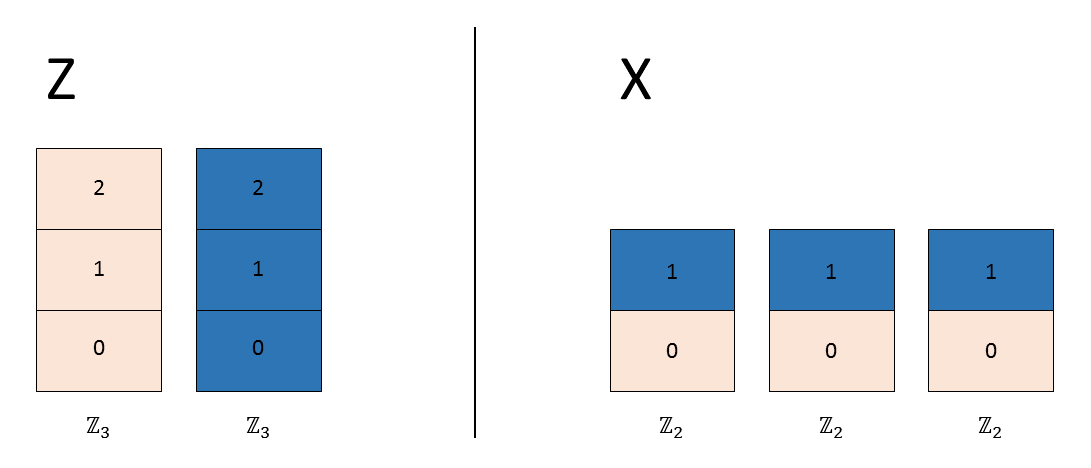
\includegraphics[height=10em,natwidth=1091,natheight=468,scale=1]{images/complexample.png}
\end{center}
\vspace{-14pt}
\caption[An example of two complementary bases on the system of six elements.]{An example of two complementary bases on the system of six elements. Here $Z=\mathbb{Z}_3\oplus\mathbb{Z}_3$ and $X = \mathbb{Z}_2\oplus\mathbb{Z}_2\oplus \mathbb{Z}_2$.  The two classical states of $Z$ are each three element subsets and are colored in pink and blue. The unbiased states of $X$ to which they correspond are colored to match.
}
\label{complEx}
\end{figure}

\begin{corollary}[\cite{evans2009classifying}]
The \textbf{classical states} of a basis $Z = \bigoplus^{N}G$ are the subsets corresponding to the groups $G_0, G_1,...$ where we forget the group structure. They will often be denoted $\ket{G_i}$.
\end{corollary}

\begin{corollary}[\cite{evans2009classifying}]
The \textbf{unbiased states} for a basis $Z = \bigoplus^{N}G$ are subsets $U$ such that for a fixed $g\in G$, $\ket{U} = \bigoplus^{N}\{g\}$.
Thus there is exactly one element in each unbiased $U$ from each component $G_i$ of $Z$.
\end{corollary}

\begin{example}
Take $Z = \mathbb{Z}_2\oplus\mathbb{Z}_2=\{0_a,1_a,0_b,1_b\}$. The classical states of $Z$ are $\ket{G_a}=\ket{0_a\vee1_a}$ and $\ket{G_b}=\ket{0_b\vee1_b}$.  The unbiased states of $Z$ are $\ket{U_0}=\ket{0_a\vee0_b}$ and $\ket{U_1}=\ket{1_a\vee1_b}$.
\end{example}

It is easy to check that bases as specified by Theorem \ref{thm:compl} have the property that each classical state $\ket{G_i}$ of the basis $Z$ corresponds to one unbiased state of $X$ and vice versa.
This allows us to call these bases mutually unbiased, i.e. complementary~\cite{evans2009classifying}.
\subsubsection*{Phases}

Phases are also defined in this relational setting.  In Hilbert space quantum mechanics a quantum phase for an n-dimensional system is given by the vector
\begin{align*}
\left(\begin{array}{c}
e^{i\phi_1} \\
\vdots \\
e^{i\phi_n}
\end{array}
\right).
\end{align*}
These quantum phases form an abelian group and can be applied as phase gates.
Their relational counterparts are described by the following lemma from \cite{cqm-notes}:
\begin{lemma}
For a basis $Z=\bigoplus_i^NG_i$, the \textbf{phase group} $B(Z)$ is given by $\prod_i^NG_i$.
\end{lemma}

\begin{example}
Consider the basis $\mathbb{Z}_2\oplus\mathbb{Z}_2$ for the four element system $\{00,01,10,11\}$.  Let $|\psi\rangle$ be the state $|00\vee10\rangle$. Application of the phase $11$ results in
\[ 11|00\vee10\rangle = |11\vee01\rangle . \]
\end{example}

We are also able to interpret GHZ states and density matrices in sets and relations.

\begin{defn}
For a basis $Z$, a \textbf{GHZ} state is given by
\[ GHZ_Z \; := \{\;(a,b,c)\;|\;\ \forall \;a,b,c \in Z,\;a\bullet_Zb\bullet_Zc = \mbox{id}_{G_i}\mbox{ for some } i\;\}.  \]
\end{defn}

\begin{defn}
For a state $|\psi\rangle$, the \textbf{density matrix} $|\psi\rangle\langle\psi|$ is given by the relation $xRy$ s.t. $x,y\in \psi$.
\end{defn}

\subsubsection*{The Model QCRel}

\begin{defn}
Axioms 1-4, and subsequent definitions, specify the operational generalized compositional theory for \textbf{quantum computation in relations: QCRel}.
\end{defn}

By the oGCT construction, this clearly makes QCRel a model of quantum computation in sets and unitary relations. It is worth noting that QCRel can be simply viewed as a local hidden variable theory. Consider the set $H$ to be the set of ontic states such that for $\phi\subseteq H$ the state $\ket{\phi}$ is non-deterministically in any of the ontic states in the subset $\phi$.  From this perspective, QCRel provides a non-deterministic local hidden variable model for computational aspects of quantum mechanics \cite{abramsky2012operational}. This means that protocols exist for entanglement, teleportation, and, as we show in this section, some familiar blackbox algorithms.

\subsection{Unitary Oracles}

In order to model blackbox quantum algorithms in this setting, we must define the oracles themselves.
We do this by building up from an abstract definition of the controlled-not gate in the literature. Let the gray classical structure on a system $A$ be given by a basis $Z=\bigoplus^{|H|}G$ and the white classical structure be a basis $X=\bigoplus^{|G|}H$. The comonoid for the gray dot is then the relation $\tinycomult[graydot]:A\to A\times A$ that for $x,a,b\in H$ is given by
\[ \{(x,(a,b))~|~a\bullet_Zb=x\}. \]

\begin{defn}[\cite{zeng2014abstract}]
\label{eq:generalizedcnotrel}
The abstract controlled-not is given by a composition of the comonoid for Z and the monoid for X:
\begin{equation}
\label{eq:cnot_rel}
\,\,
\begin{aligned}
\begin{tikzpicture}[yscale=0.6, xscale=0.6,string]
\node (b) [graydot] at (0,0) {};
\node (w) [whitedot] at (1,1) {};
\draw (-0.75,2) to [out=down, in=left] (b.center);
\draw (b.center) to [out=right, in=left] (w.center);
\draw (w.center) to (1,2);
\draw (b.center) to (0,-1);
\draw (w.center) to [out=right, in=up] (1.75,-1);
\end{tikzpicture}
\end{aligned}
\qquad \qquad\qquad
\begin{tabular}{l}
\mbox{CNOT:} $H\times H\to H\times H ::$ \\
$\{((x,y),(a,b\circ_Xy))~|~a\bullet_Zb=x\}.$ \\
\end{tabular} 
\end{equation}
\end{defn}
It can be shown that in the traditional quantum setting of Hilbert spaces and linear maps, this exactly corresponds to the usual controlled-not. This also leads to the following useful theorem, which can be abstractly proved.

\begin{theorem}[Complementarity via a unitary \cite{zeng2014abstract}]
\label{thm:complementarityunitary}
  Two symmetric dagger-Frobenius algebras are complementary if and only if the abstract controlled-not from Definition \ref{eq:generalizedcnotrel} is unitary.
\end{theorem}

\noindent This allows us to prove the following about  complementary bases in QCRel.
\begin{theorem}
Two bases (Z and X) in QCRel are complementary, in the sense of Theorem~\ref{thm:compl}, if and only if the relation in \eqref{eq:cnot_rel} is a bijection.
\end{theorem}
\begin{proof}
The relevant relation can clearly be seen to be the composite in Definition~\ref{eq:generalizedcnotrel} as:
\begin{align}
\{((a,b,y),(a,b\circ_Xy))\} \circ \{((x,y),(a,b,y))~|~a\bullet_Zb=x\}.
\end{align}
Thus the abstract proof of\ Theorem \ref{thm:complementarityunitary} from \cite{zeng2014abstract} goes through unchanged.
\end{proof}

An oracle is then introduced as a controlled-not where we have embedded a particular kind of relation that abstractly must be a self-conjugate comonoid homomorphism \cite{zeng2014abstract}. We construct such relations in the following lemmas.

\begin{defn}
Let $G$ and $H$ be groupoids with with groupoid multiplications $\bullet_G$ and $\bullet_H$ respectively. Let $\mbox{id}_{G}=\bigcup_{X\in\mbox{Ob}(G)}\mbox{id}_X$ and similarly define $\mbox{id}_{H}$. A \textbf{groupoid homomorphism relation} $R:G\to H$ obeys the following condition for $g_1,g_2\in G$:
%two conditions for $g_1,g_2\in G$ and $h_1,h_2\in H$:
\begin{align}
R(g_1\bullet_Gg_2) &= R(g_1)\bullet_HR(g_2) %\\
%R(\mbox{id}_G) &= \mbox{id}_H
\end{align}
\end{defn}
\noindent Note that while this in many ways resembles a groupoid homomorphism, it is actually a weakening of this notion, in that groupoid homomorphism relations are not required to be total functions and have no explicit requirement on their identity morphisms.

\begin{defn}
A \textbf{monoid homomorphism relation} is a monoid homomorphism in \cat{Rel}. Specifically, let $A$ and $B$ be sets equipped with monoids $(A,\tinymult[whitedot],\tinyunit[whitedot])$ and $(B,\tinymult[blackdot],\tinyunit[blackdot])$ respectively. A relation $r:A\to B$ is a monoid homomorphism when is obeys the following two conditions:
\begin{align}
\label{eq:monone}
r\circ\tinymult[whitedot] &= \tinymult[blackdot]\circ(r\times r) 
\end{align}
\begin{align}
\label{eq:monunit}
r\circ\tinyunit[whitedot] &= \tinyunit[blackdot]
\end{align}
A \textbf{comonoid homomorphism relation} is defined similarly, using duals of the above conditions.
\end{defn}

\begin{lemma}
\label{lem:mongrphom}
A groupoid homomorphism relation that is surjective on objects is a monoid homomorphism relation.
\end{lemma}
\begin{proof}
Throughout this proof we refer to a groupoid as a category where the elements of the groupoid are the morphisms.  From this perspective a group is a groupoid with a single object. Consider a groupoid homomorphism relation $R:G\to H$ on objects $X,A,B$ of $G$ and morphisms $f$ of $G$.
In order to show that $R$ is a monoid homomorphism relation we first show that it preserves the unit~\eqref{eq:monunit}. We have $R(\bigcup_{X\in\mbox{Ob}(G)} \mbox{id}_X) = \bigcup_{Y\in\mbox{Ob}(H)} \mbox{id}_Y$. Recall that for a set $A$,  $R(A)=\bigcup_{a\in A} R(a)$. It is that case that
\begin{align}
R(\bigcup\nolimits_{X\in\mbox{Ob}(G)} \mbox{id}_X) &= \bigcup\nolimits_{X\in\mbox{Ob}(G)}R(\mbox{id}_X) = \bigcup\nolimits_{X\in\mbox{Ob}(G)}\mbox{id}_{R(X)} \quad \mbox{def. of group hom. rel.} \\
&= \bigcup\nolimits_{R(X)\in\mbox{Ob}(G)}\mbox{id}_{R(X)} = \bigcup\nolimits_{{Y\in\mbox{Ob}(H)}}\mbox{id}_{Y} \qquad \mbox{surjective on objects}
\end{align}
where we have used the fact that $R$ is surjective on objects, which implies that every object of $H$ is in the image of $R$ and that $|\mbox{Ob}(G)|\ge|\mbox{Ob}(H)|$.

The second monoid homomorphism condition~\eqref{eq:monone} is to preserve multiplication, i.e. that for subsets $K$ and $J$ of $G$ we have
\begin{align}
R(K+_GJ)=R(K)+_HR(J).
\end{align}

\noindent Here we recall that for two sets $A$ and $B$, $A+B=\{a + b | a \in A\mbox{ and } b \in B\}$. Thus,
\begin{align}
R(K+_GJ) &= R(\bigcup\nolimits_{k\in K,j\in J}k+_Gj) = \bigcup\nolimits_{k\in K,j\in J}R(k+_Gj) \\
&= \bigcup\nolimits_{k\in K,j\in J}R(k)+_HR(j) \qquad \mbox{def. of group hom. rel.}\\
&= R(K)+_HR(J).
\end{align}
This completes the proof.
\end{proof}

We then dualize the proof of Lemma \ref{lem:mongrphom} to conclude that:
\begin{lemma}
\label{lem:classicalRelation}
Let $F:H\to G$ be a functor such that $F^{\mbox{\tiny op}}$ is a groupoid homomorphism relation that is surjective on objects. $F$ is a comonoid homomorphism relation.
\end{lemma}
\noindent We call these comonoid homomorphism relations \textbf{classical relations}. These are relations that properly preserve the structure of the bases where classical data is embedded.  In the quantum case they take basis elements to basis elements. Some examples in QCRel are listed in Appendix \ref{app:clRel}. In order to define unitary oracles, we also need these relations to be self-conjugate:

\begin{defn}[\cite{zeng2014abstract}]
In a monoidal dagger-category, a comonoid homomorphism \mbox{$f:\blackcomonoid{A} \to \graycomonoid{B}$} between dagger-Frobenius comonoids is \textbf{self-conjugate} when the following property holds:
\begin{equation}
\label{eq:comonoidhomomorphismselfconjugate}
\begin{aligned}
\begin{tikzpicture}[yscale=0.8, xscale=0.8, thick]
\node [morphism] (f) at (2,1) {$f$};
\draw (0,-1) to [out=up, in=left, in looseness=0.9] (1,2) node [graydot] {} to (1,2.5) node [graydot] {};
\draw (1,2) to [out=right, in=up] (f.north);
\draw (f.south) to [out=down, in=left] (3,0) node [blackdot] {} to [out=right, in=down, out looseness=0.9] (4,3);
\draw (3,0) to (3,-0.5) node [blackdot] {};
\node [graydot] at (1,2) {};
\end{tikzpicture}
\end{aligned}
\quad=\quad
\begin{aligned}
\begin{tikzpicture}[yscale=1.05, xscale=0.8, thick]
\node (f) at (0,0) [morphism] {$f^{\dagger}$};
\draw (0,-1.5) to (f.south);
\draw (f.north) to (0,1.5);
\end{tikzpicture}
\end{aligned}
\end{equation}
\end{defn}
The meaning of this equation in relations is explicated in the following lemma.

\begin{lemma}
All classical relations $f:Z^A\to Z^B$ between groupoids $Z^A=\bigoplus^NG$ and $Z^B=\bigoplus^{N'}H$ are self-conjugate.
\end{lemma}
\begin{proof}
In QCRel, our dagger-Frobenius structures are groupoids and, if they are complementary to some other groupoid, then they are of the form $Z^A=\bigoplus^NG$ and $Z^B=\bigoplus^{N'}H$. We annotate the definition of self-conjugacy for some arbitrary element $(g,n)$, the element $g$ from the $n$-th group. Recall that $f^{\dagger}=f^{-1}$ in QCRel.
\begin{equation}
\begin{aligned}
\begin{tikzpicture}[yscale=0.9, xscale=1.3, thick]
\node [morphism] (f) at (2,1) {$f$};
\draw (0,-1) to [out=up, in=left, in looseness=0.9] (1,2) node [graydot] {} to (1,3.3) node [graydot] {};
\draw (1,2) to [out=right, in=up] (f.north);
\draw (f.south) to [out=down, in=left] (3,-0.7) node [blackdot] {} to [out=right, in=down, out looseness=0.9] (4,3);
\draw (3,-0.7) to (3,-2) node [blackdot] {};
\node [graydot] at (1,2) {};
\node at (0,-1.25) {\small $(g,n)$};
\node at (-0.25,1.5) {\small $(g,n)$};
\node at (0.9,2.65) {\small $\{(id_G,j) | 1 \leq j \leq N\}$};
\node at (2.5,1.7) {\small $(g^{-1},n)$};
\node at (2.1,-0.15) {\small $f^{-1}(g^{-1},n)$};
\node at (4.3,0) {\small $\left[f^{-1}(g^{-1},n)\right]^{-1}$};
\node at (2.95,-1.4) {\small $\{(id_H,k) | 1 \leq k \leq N'\}$};
\end{tikzpicture}
\end{aligned}
\quad=\quad
\begin{aligned}
\begin{tikzpicture}[yscale=1.2, xscale=1.3, thick]
\node (f) at (0,0) [morphism] {$f^{-1}$};
\draw (0,-1.5) to (f.south);
\draw (f.north) to (0,1.5);
\node at (0,-2) {\small $(g,n)$};
\node at (0,2) {\small $f^{-1}(g,n)$};
\end{tikzpicture}
\end{aligned}
\end{equation}
Thus, a relation $f$ is self-conjugate if and only if for all elements $(g,n)$ it is the case that $[f^{-1}(g^{-1},n)]^{-1}=f^{-1}(g,n)$. From Lemma \ref{lem:classicalRelation} the converse of the classical relation $f$ is a monoid homomorphism relation whose multiplication is the groupoid operation, so this condition will hold.
\end{proof}

Classical relations, as self-conjugate comonoid homomorphisms, lead to unitary oracles.

\begin{defn}[Oracle \cite{zeng2014abstract}]
\label{oracle}
Given a groupoid $Z^A:\blackcomonoid{A}$, a pair of complementary groupoids $Z^B:\graycomonoid{B}$ and $X^B:\whitecomonoid{B}$, and a classical relation $R : \blackcomonoid{A} \to \graycomonoid{B}$, an \textbf{oracle} is defined to be the following endomorphism of~$A \times B$:
\begin{equation}
\label{eq:oraclerel}
\begin{aligned}
\begin{tikzpicture}[string,xscale=0.9, yscale=0.7]
    \node (dot) [blackdot] at (0,1) {};
    \node (f) [morphism] at (0.7,2) {$R$};
    \node (m) [whitedot] at (1.4,3) {};
\draw (0,0.25)
        node [below] {$A$}
    to (0,1)
    to [out=left, in=south] (-0.7,2)
    to (-0.7,3.75)
        node [above] {$A$};
\draw (0,1)
    to [out=right, in=south] (f.south);
\draw  (f.north)
    to [out=up, in=left] (1.4,3)
    to [out=right, in=up] +(0.7,-1)
    to (2.1,0.25)
        node [below] {$B$};;
\draw (m.center) to +(0,0.75) node [above] {$B$};
\end{tikzpicture}
\end{aligned}
\qquad \qquad
\begin{align*}
&\mbox{\emph{OracleRel(R)}}:A\times B\to A\times B  ::\\
&\{((x,y),(a,c\circ_Xy))~|~ \\ &\hspace{50pt}\exists b\in A, s.t.~a\bullet_{Z^A}b=x\mbox{\emph{ and }} bRc\}. \\
\end{align*}
\end{equation}
\end{defn}
\begin{theorem}
\label{thm:familyofunitaries}
Oracles are unitary.
\end{theorem}
\begin{proof}
Proved in the abstract setting for Definition \ref{oracle} in \cite{zeng2014abstract}, when $R$ is a self-conjugate comonoid homomorphism.  Though there are others, classical relations $R$ are necessary and sufficient in our cases as the algorithms that follow additionally require that the comonoids be part of classical structures.
\end{proof}

\begin{corollary}
OracleRel is a bijection.
\end{corollary}
\begin{proof}
This follows directly from Theorem \ref{thm:familyofunitaries} and Corollary \ref{cor:bijections}.
\end{proof}

\subsection{The Fourier Transform in Relations}
\label{sec:RelFT}

In Section~\ref{section_RelFT}, we saw that there are several perspectives on the Fourier Transform in \cat{FRel}, only some of which are nontrivial. In this section we take the operational perspective on the generalized quantum Fourier transform whose definition is motivated through the relationship between classical and unbiased states of two bases.  For abelian groups $G$ and $H$, consider two groupoids $Z=\bigoplus^{|H|}G$ and $X=\bigoplus^{|G|}H$ to be complementary bases of the same system.

\begin{defn}
\label{def:FTRel}
The \textbf{quantum Fourier transform in relations} corresponds to preparing classical states of $Z$ and measuring them against classical states of $X$.
%is an isomorphism from the classical states of $Z$ to the unbiased states %of $X$, i.e.
%\begin{align*}
%\{G_h\}\mapsto \{h_g|\forall g\in G\}
%\end{align*}
\end{defn}

\begin{example}
Take $G=\mathbb{Z}_2=\{0,1\}$, $H=\mathbb{Z}_1=\{\star\}$, $Z = G$ and $X=H\oplus H = \{ (\star,0),(\star,1) \}$. The computational basis is the family $\ket{H_g}_{g\in G}$ of classical states for $X$, i.e. $H_0 = \{(\star,0)\}$ and $H_1 = \{(\star,1)\}$. The quantum Fourier basis is a single classical state $G_\star = \{(\star,0), (\star,1)\}$ for $Z$. In this case all states can be prepared in the computational basis, but  measurement in the quantum Fourier basis is trivial.
\end{example}

\begin{example}
Take $G=\mathbb{Z}_2=\{0,1\}$, $H=\mathbb{Z}_2=\{a,b\}$, $Z = G \oplus G = \{ (0,0),(1,0),(0,1),(1,0)\}$ and $X= H \oplus H = \{ (a,a), (b,a), (a,b), (b,b) \}$. The computational basis is the family $\ket{H_g}_{g \in G}$ of classical states for $X$, i.e. $H_0 = \{(a,a),(b,a)\}$ and $H_1 = \{(a,b),(b,b)\}$. The quantum Fourier basis is the family $\ket{G_h}_{h\in H}$ of classical states for $Z$, i.e. $G_a = \{(0,0),(0,1)\}$ and $G_b = \{(1,0),(1,1)\}$.
\end{example}

See Section~\ref{sec:strcomplFT} and~\cite{gogioso2015fourier} to fully motivate this definition of the Fourier transform in QCRel and for its relationship to the usual Hadamard and Fourier transforms for Hilbert spaces and linear maps.

\subsection{The Deutsch-Jozsa Algorithm in QCRel}

The well known Deutsch-Jozsa algorithm is an early quantum algorithm that demonstrates a speedup over exact classical computation \cite{DJAlg1992}. It takes as input a function promised to be either constant or balanced and returns which, deterministically using only a single oracle query. In this section, we model the algorithm's steps in QCRel just as it is implemented with Hilbert spaces and linear maps. This approach is somewhat dual to the usual one where different algorithms are compared on the same problem. Here we run the same abstract protocol (implemented in a different model) with the same query complexity and compare the different problems that it solves.

To run this algorithm in QCRel we use two systems.  System $A$ has cardinality $n$ and system $B$ has cardinality $\ge 2$. Take $Z^A=\bigoplus^{|H^{A}|}G^A$ and $X^A=\bigoplus^{|G^{A}|}H^A$ to be complementary bases of $A$. Take $Z^B=\bigoplus^{|H^{B}|}G^B$ and $X^B=\bigoplus^{|G^{B}|}H^B$ to be complementary bases of $B$, such that $X^B$ has at least two classical states. In analogy with the usual specification, the algorithm proceeds with the following steps.
\begin{enumerate}
\item Prepare $A$ in the zero state $|G^{A}_0\rangle$. Prepare $B$ in the state given by the second classical state of $Z^B$, i.e. $|G^B_1\rangle$.

\item Apply the Fourier transform, as given by Definition \ref{def:FTRel}, to each system, resulting in states $\ket{H_0^A}$ and $\ket{H_1^B}$ respectively.

\item Apply an oracle \eqref{eq:oraclerel}, built from a classical relation $f:Z^A\to Z^B$.

\item Again apply the Fourier transform to system $A$ and then measure it in the $Z$ basis.
\end{enumerate}

\noindent This sequence of steps is an instance in sets and relations of the abstract Deutsch-Jozsa algorithm from \cite{vicary-tqa}, which translates to the following relation, where we have already applied the Hadamard map  to the input and output. See~\eqref{eq:postFT}.

\begin{equation}
\label{eq:reldj}
\begin{aligned}
\begin{tikzpicture}[string, yscale=1, xscale=1]
    \node (dot) [blackdot] at (0,1) {};
    \node (f) [morphism] at (0.7,2) {$f$};
    \node (m) [whitedot] at (1.4,3) {};
\draw (0,0.25)
        node [blackdot] {}
    to (0,1)
    to [out=left, in=south] (-0.7,2)
    to (-0.7,3.75)
        node [blackdot] {};
\draw (0,1)
    to [out=right, in=south] (f.south);
\draw  (f.north)
    to [out=up, in=left] (1.4,3)
    to [out=right, in=up] +(0.7,-1)
    to (2.1,0.25)
        node [graydot] {};
\node at (2.15,0.25) [anchor=west] {$|H^B_1\rangle$};
\node at (0.05,0.25) [anchor=west] {$|H^A_0\rangle$};
\node at (-0.65,3.75) [anchor=west] {$\langle H^A_0|$};
\draw (m.center) to +(0,0.75)
        node [above] {};
\draw [thin, dashed] (-1.25,0.7) to (7.5,0.7);
\draw [thin, dashed] (-1.25,3.3) to (7.5,3.3);
\node at (3.5,0) [anchor=west] {\small Prepare initial states and apply Hadamard};
\node at (3.5,2) [anchor=west] {\small Apply a unitary map};
\node at (3.5,4) [anchor=west] {\small Apply Hadamard and measure the first system};
\end{tikzpicture}
\end{aligned}
\end{equation}
that is explicitly written as:
\begin{align*}
\mbox{DJAlg}(f)&::\{\star\}\times \{\star\} \to \{\star\}\times B \\
&=
\bra{H_0^A}\times{\mbox{id}_B}\circ\mbox{OracleRel}(f)\circ\ket{H^A_0}\times\ket{H^B_1}
\\ &=
\{((\star,\star),(\star,z))\;|\; 
  z\in H_1^B \mbox{ and } \exists y\in H_0^A, \mbox{ s.t. }yfz\},
\end{align*}
where we have made the simplification of \eqref{eq:reldj} following \cite{vicary-tqa}.

\begin{theorem}[\cite{vicary-tqa}]
\label{def:bc}
In any dagger compact category with complementary bases, the algorithm in Equation \ref{eq:reldj} will, with a single oracle query, distinguish \textbf{constant} and \textbf{balanced} classical relations $f:Z^A\to Z^B$ according to the following abstract definitions. Here $\ket{x}$ is a classical point of $Z^A$ and the zero scalar $0$ is, in \cat{Rel}, the empty relation:
\begin{equation}
\label{eq:bc}
\mbox{\\ constant}:\quad
\begin{aligned}
\begin{tikzpicture}[scale=1]
\node (f) [morphism] at (0,0) {$f$};
\draw (0,-1) to (f.south);
\draw (f.north) to (0,1);
\end{tikzpicture}
\end{aligned}
\;=\;
\begin{aligned}
\begin{tikzpicture}[scale=1]
\draw (0,-1) to (0,-.4)
    node [blackdot] {};
\draw (0,0.5) node [state] {$x$} to (0,1);
\end{tikzpicture}
\end{aligned}
=\ket{x}\circ\tinycounit[blackdot]
\qquad\qquad \mbox{balanced:\quad}
\begin{aligned}
\begin{tikzpicture}[string, scale=1]
\node [morphism] (f) at (0,0) {$f$};
\draw (0,-0.85) node [blackdot] {} to (f.south);
\draw (f.north) to (0,0.75) node [graydot, hflip] {};
\node at (0.05,0.75) [anchor=west] {$2$};
\end{tikzpicture}
\end{aligned}
\quad=\quad
0, \vspace{-5pt}
\end{equation}
where 
\begin{tikzpicture}[string, yscale=1]
\draw (f.north) to (0,0.75) node [graydot, hflip] {};
\node at (0.05,0.75) [anchor=west] {$2$};
\end{tikzpicture} is the dagger adjoint of the second classical state of $X^B$.
\end{theorem}
That these definitions coincide with the usual ones for constant and balanced functions is shown in \cite{vicary-tqa}. In QCRel, the effect 
\begin{tikzpicture}[string,scale=0.75]
\draw (f.north) to (0,0.75) node [blackdot, hflip] {};
%\node at (0.05,0.75) [anchor=west] {$2$};
\end{tikzpicture} is $\langle H^A_1|$, which acts as a measurement of system $A$ after applying the oracle.
We illustrate the details of the QCRel model of this algorithm by example and then with general definitions.

\begin{example}
Take $A=\{0,1,2,3\}$ and $B=\{a,b,c,d\}$ to be four element systems. We define complementary bases on these systems as the following:
\begin{align*}
\begin{tabular}{|c|c|}\hline
System $A$ & System $B$ \\\hline
$Z^A = \mathbb{Z}_2\oplus\mathbb{Z}_2 \mbox{~~s.t.}$ & $Z^B = \mathbb{Z}_2\oplus\mathbb{Z}_2\mbox{~~s.t.}$ \\
$G_0^A=\{0,1\},G_1^A=\{2,3\}$ & $G_0^B=\{a,b\},G_1^B=\{c,d\}$ \\ \hline
$X^A = \mathbb{Z}_2\oplus\mathbb{Z}_2 \mbox{~~s.t.}$ & $X^B = \mathbb{Z}_2\oplus\mathbb{Z}_2\mbox{~~s.t.}$ \\
$H_0^A=\{0,2\},H_1^A=\{1,3\}$ & $H_0^B=\{a,c\},H_1^B=\{b,d\}$ \\ \hline
\end{tabular}
\end{align*}


From Equation \ref{eq:bc}, we then define constant and balanced classical relations using the following dictionary:
\begin{align}
\begin{aligned}
\begin{tikzpicture}[string]
\draw (0,0.2) to (0,0.75) node [blackdot, hflip] {};
\node at (0.05,0.75) [anchor=west] {};
\end{tikzpicture}
\end{aligned}
&\quad= \{(0,\star),(2, \star)\},  \quad \mbox{the adjoint of the first classical state of } X^A \\
\begin{aligned}
\begin{tikzpicture}[string]
\node (x) [state, xscale=0.75] at (0,0) {$x$};
\draw (0,0) to (0,0.5) {};
\end{tikzpicture}
\end{aligned}
&\quad= \{(\star,a),(\star,b)\}\mbox{ OR }\{(\star,c),(\star,d)\},  \quad \mbox{a classical state of }Z^B \\
\begin{aligned}
\begin{tikzpicture}[string]
\draw (0,0.2) to (0,0.75) node [graydot, hflip] {};
\node at (0.05,0.75) [anchor=west] {$2$};
\end{tikzpicture}
\end{aligned}
&\quad=\{(b,\star),(d, \star)\},  \quad \mbox{ adjoint of the second classical state of } X^B \\
\begin{aligned}
\begin{tikzpicture}[string]
\node (x) [blackdot] at (0,0) {};
\draw (0,0) to (0,0.5) {};
\end{tikzpicture}
\end{aligned}
&\quad= \{(\star,0),(\star,2)\},  \quad \mbox{the first classical state of } X^A
\end{align}

Thus there are two constant classical relations\footnote{A list of more example classical relations is given in Appendix \ref{app:clRel}.} $f:Z^A\to Z^B$, one for each classical state of $Z^B$. They are:
\begin{align*}
\{ (0,a),(0,b) ,(2,a),(2,b) \} \quad \mbox{and} \quad
\{ (0,c),(0,d), (2,c),(2,d) \}.
\end{align*}
By Definition \ref{def:bc}, balanced classical relations are those which do not relate $0$ or $2$ to either $b$ or $d$. There are four balanced classical relations for this example:
\begin{align*}
\{(0,c),(2,c),(1,d),(3,d)\} &\qquad \{(0,a),(1,b),(2,c),(3,d)\} \\
\{(2,a),(3,b),(0,c),(1,d)\} &\qquad \{(0,a),(2,a),(1,b),(3,b)\} \\
\end{align*}
For a classical relation promised to be in one of these two classes, we can distinguish which with a single oracle query.
\end{example}

We generalize these definitions of constant and balanced classical relations to the following:
\begin{defn}
\label{def:const}
Let $Z^A=\oplus^NG_i$. A \textbf{constant relation} $f:Z^{A}\to Z^{B}$ relates all id$_{G_i}$ to a single classical state of $Z^B$.
\end{defn}

\begin{defn}
\label{def:balanced}
A relation $f:Z^{A}\to Z^{B}$ is \textbf{balanced} when no element in the first classical state of $X^{A}$ is related to an element in the second classical state of $X^{B}$.
\end{defn}

\begin{theorem}
\label{thm:dj_speedup}
The Deutsch-Jozsa algorithm defined above distinguishes constant relations from balanced relations in a single oracle query.
\end{theorem}
\begin{proof}
This follows immediately from the abstract proof of the Deutsch-Jozsa algorithm in \cite{vicary-tqa}.
\end{proof}

This result shows that we are able to model the Deutsch-Jozsa algorithm in the nondeterministic classical setting of QCRel.

\subsection{Single-shot Grover's Algorithm}

The usual Grover's algorithm~\cite{grover1996fast} takes as input a set $S$ and an indicator function $f:S\to\{0,1\}$ and outputs an element $s\in S$ such that $f(s)=1$. Though the algorithm is usually probabilistic and runs a repeated series of ``Grover steps", here we consider the deterministic version that runs with a single step. In this section we will consider the generalization of the single-shot Grover algorithm where the codomain of the indicator function is allowed to be an arbitrary group~\cite{vicary-tqa}. Our setup requires the set $S$, as one system, as well as another system $B$. We define the basis $Z^{S}=\bigoplus^{|H^S|}G^S$ and $X^S=\bigoplus^{|G^S|}H^S$ on the $S$ system.  System $B$ has complementary bases $Z^B=\bigoplus^{|H^B|}G^B$ and $X^B=\bigoplus^{|G^B|}H^B$. Let $\ket{\sigma}$ be the first classical state of $X^B$, e.g. is $X^B=\mathbb{Z}_2\oplus\mathbb{Z}_2$ then $\ket{\sigma}=\{(\star,1),(\star,3)\}$, where $1$ and $3$ are the non-identity elements of that factors of $X^B$. Let $\bra{\rho}$ be the converse of a classical state of $X^S$. Recall that $\ket{G^S_0}=\{(\star,g)\,|\,g\in G^S\mbox{ is the first factor group of } Z^S\}$ is a classical point of $Z^S$, and that, by the complementary relationship of classical and unbiased points (Section~\ref{sec:RelFT}), $\ket{H^S_0}\isom\{(\star,\idm{G^S_i})\,|\,G^S_i\mbox{ is a factor group of } Z^S\}$.

In QCRel, the algorithm proceeds by the following steps:
\begin{enumerate}
\item Prepare system $S$ in the state $\ket{G_0}$ and system $B$ in the state $\ket{\sigma}$.

\item Apply the Fourier transform to system $S$, resulting in state $\ket{H^{S}_0}$.

\item Apply the oracle for a classical indicator relation $f:Z^S\to Z^B$.

\item Apply a diffusion relation $D:S\to S$ (defined below) to system $S$.

\item Measure system $S$ in the $X^S$ basis.

\end{enumerate}

The diagrammatic presentation for this procedure from \cite{vicary-tqa} is:
\begin{equation}
\label{eq:grovertopological}
\begin{aligned}
\begin{tikzpicture}[thick, xscale=1, yscale=0.5]
\begin{pgfonlayer}{foreground}
    \node (f) [smallbox, anchor=south, thick] at (0.7,2) {$f$};
\end{pgfonlayer}
    \node (dot) [blackdot] at (0,1) {};
    \node (m) [whitedot] at ([xshift=0.7cm, yshift=1cm] f.north) {};
\draw (0,-0.25)
        node [blackdot] (bdot) {}
    to (0,1)
    to [out=\nwangle, in=south] (-0.7,2)
    to ([yshift=1.4cm] m.center -| -0.7,1)
        node (rho) [state,hflip,yscale=1.5, xscale=1.1] {};
\node at (-0.7,5.9) {$\bra{\rho}$};
\draw (0,1)
    to [out=\neangle, in=south] (f.south)
    to (f.north)
    to [out=up, in=\swangle] +(0.7,1)
    to [out=\seangle, in=up] +(0.7,-1)
    to (2.1,-0.25)
        node [state,yscale=1.5, xscale=1.1] (sigmadag) {};
\node at (2.1,-1) {$\ket{\sigma}$};        
\draw (m.center) to (1.4,5.75)
        node [above] {};
\node [smallbox] at (-0.7,3.5) {$D$};
\node at (3.5,-0.25) [anchor=west] {Preparation};
\draw [thin, dashed] (-2,0.6) to (7,0.6);
\node at (3.5,2.25) [anchor=west] {Dynamics};
\draw [thin, dashed] (-2,4.5) to (7,4.5);
\node at (3.5,5) [anchor=west] {Measurement};
\end{tikzpicture}
\end{aligned}
\end{equation}

\noindent where numerical scalars have been dropped relative to that reference as there is only one non-zero scalar in QCRel.\footnote{Recall that scalars in a monoidal category with identity object $I$ are maps $s:I\to I$. Thus in \cat{Rel} $I=\{\star\}$, so the only scalars are the empty relation and the identity relation on the singleton set.} Recall that $\tinyunit[blackdot]:\{\star\}\to S$ relates the singleton to the elements of $H_0$ and that $\tinycounit[blackdot]$ is its relational converse. We will use the map $\tinyunit[blackdot]\circ\tinycounit[blackdot]:S\to S$ in the following definition. Here there is a special relation $D:S\to S$ called the diffusion operator and defined abstractly in \cite{vicary-tqa}:
\begin{equation}
\label{eq:difftopological}
\begin{aligned}
\begin{tikzpicture}[thick, scale=1]
\draw (0,0) node [below] {$S$} to node [smallbox] {$D$} (0,2) node [above] {$S$};
\end{tikzpicture}
\end{aligned}
\hspace{5pt}\;=\;\hspace{5pt}
\hspace{-5pt}
\begin{aligned}
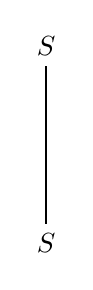
\begin{tikzpicture}[thick, scale=1]
\draw (0,0) node [below] {$S$} to (0,2) node [above] {$S$};
\end{tikzpicture}
\end{aligned}
\;-\;
\begin{aligned}
\begin{tikzpicture}[thick, scale=1]
\draw (0,0) node [below] {$S$} to (0,0.7) node [blackdot] {};
\draw (0,2) node [above] {$S$} to (0,1.3) node [blackdot] {};
\end{tikzpicture}
\end{aligned}
\qquad\qquad \qquad D := \{(x,x)\,|\,x\in S\}\bigtriangleup (H_0\times H_0)
\end{equation}
where the subtraction of two relations is given by the symmetric difference of their images. Explicitly then, the relational model for Grover's algorithm is:
\begin{align*}
\mbox{Grover}(f)&:\{\bullet\}\times \{\bullet\} \to \{\bullet\}\times B \\
&=
\bra{\rho}\times{\mbox{id}_B}\circ D\times{\mbox{id}_B}\circ\mbox{OracleRel}(f)\circ\ket{H^S_0}\times\ket{\sigma}
\\ &= \{((\bullet,\bullet),(\bullet,c\circ_{X}x))\;|\; \\
&\hspace{40pt}
 x\in\sigma,y\in\rho, \mbox{id}_{G_n},b,z\in S \mbox{ s.t. } z\bullet_{Z^S} b=\mbox{id}_{G_{n}} \mbox{ and } bfc,zDy\}
\end{align*}

\begin{theorem}
\label{thm:topgrovers}
Equation \ref{eq:grovertopological} is zero only for classical states of $X^S$ denoted $\ket{\rho}$ that satisfy the following equation:
\begin{equation}
\label{eq:zerocondition}
\sigma \circ f \circ \rho = \sigma \circ f \circ \ket{G_0}
\end{equation}
%\begin{equation}
%\label{eq:zerocondition}
%\begin{aligned}
%\begin{tikzpicture}[thick, scale=0.5]
%\draw (0,0) node [smallbox] {$\rho$} to (0,1.25) node [smallbox] {$R$} to %(0,2.5) node [smallbox] {$\sigma$};
%\end{tikzpicture}
%\end{aligned}
%\quad=\quad
%\begin{aligned}
%\begin{tikzpicture}[thick, scale=0.5]
%\draw (0,0) node [blackdot] {} to (0,1.25) node [smallbox] {$R$} to (0,2.5) %node [smallbox] {$\sigma$};
%\node [smallbox, draw=white, fill=none] at (0,0) {};
%\draw (0,0) to (0,0.5);
%\end{tikzpicture}
%\end{aligned}
%\end{equation}
\end{theorem}
\begin{proof}
Proven in \cite{vicary-tqa}. See Section 3.2 equation (34).
\end{proof}

Here $\ket{\sigma}$ is, in general, any fixed classical state of $X^B$. This allows a generalization of the single-shot Grover's algorithm where the cardinality of system $B$ is increased as investigated in \cite{vicary-tqa}.
Consequently, the LHS of Equation \ref{eq:zerocondition} tests if any element in the classical state $\ket{\rho}$ is related to any of the elements in $\ket{\sigma}$. The RHS tests if any of the elements of $G_0$ are related to $\ket{\sigma}$.

\begin{proposition}
The QCRel single-shot Grover algorithm only returns states $\ket{\rho}$ such that for all $h \in H^S_0$, $s\in\rho$ and $x\in \sigma$
\begin{align*}
h f x \quad = \quad \neg(s f x) .
\end{align*}
In other words, the only elements that can be possibilistically measured under the QCRel Born rule (Axiom~\ref{ax:relborn}) are elements of $S$ that have the opposite mapping to $\sigma$, under the relation $f$, than elements of $H^{S}_0$.
\end{proposition}
\begin{proof}
By Theorem \ref{thm:topgrovers} and definitions.
\end{proof}

\begin{example}
Let $S=\{0,1,2,3\}$ and choose $Z^S=\mathbb{Z}_2\oplus\mathbb{Z}_2$ and $X^S=\mathbb{Z}_2\oplus\mathbb{Z}_2$ as $G$ (black) and $H$ (white) bases respectively, so that $G^{S}_0=\ket{0\vee 1}$ and $H^S_0 = \ket{0\vee 2}$. Let $B$ be the same four element system with the bases $Z^B=\mathbb{Z}_2\oplus\mathbb{Z}_2$ and $X^B=\mathbb{Z}_2\oplus\mathbb{Z}_2$ and choose $\ket{\sigma}=\ket{1\vee 3}$. The diffusion operator is then given by
\begin{align*}
D &:= \{(0,0),(1,1),(2,2),(3,3)\}-\{(0,0),(0,2),(2,0),(2,2)\}
\\&=\{(1,1),(3,3),(0,2),(2,0)\}.
\end{align*}

In this case, $D$ happens to be a bijection, it is a unitary relation and thus a possible evolution in QCRel.\footnote{This will not be the case whenever $S$ has more than two factor groups. Unitarity is a stringent condition on processes in QCRel.} Let $f$ be the classical relation\footnote{See Appendix \ref{app:clRel} for a list of classical relations $\mathbb{Z}_2\oplus\mathbb{Z}_2\to\mathbb{Z}_2\oplus\mathbb{Z}_2$.} $\{(0,2),(2,2),(1,3),(3,3)\}$, where elements of $H^S_0$ are not related to elements of $\ket{\sigma}$. Thus the above algorithm will only return classical states of $X^{S}$ that \textit{are} related, under $f$,\ to $\ket{\sigma}$.  The only possible outcome state is $\ket{1\vee 3}$.
\end{example}

\begin{example}
This is the same as the above example, but take $f$ to be the classical relation $\{(0,0),(2,0),(0,1),(2,1)\}$. As an element of $H^S_0$ is related to $\ket{\sigma}$, the algorithm will return classical states of $X^S$ which are \emph{not} mapped to $\ket{\sigma}$, i.e. the state $\ket{1\vee3}$.
\end{example}

\subsection{The Groupoid Homomorphism Promise Algorithm}

This section models the group homomorphism algorithm from \cite{zeng2014abstract} in QCRel.  The quantum version of the algorithm takes as input a blackbox function $f:G\to A$ promised to be one of the homomorphisms between group $G$ and abelian group $A$.  It then outputs the identity of the homomorphism. In that paper the full identification algorithm is built up by multiple calls to an instance of the problem for cyclic groups.\footnote{Making use of the structure theorem for abelian groups to complete the general case.} It is this cyclic group subroutine that we consider here. In the relational setting we will move from groups to groupoids. Let groupoid $H$ be complementary to groupoid $G$ and groupoid $B$ be complementary to groupoid $A$. The QCRel GroupHomID algorithm then takes as input a groupoid isomorphism $f:G\to A$.   Let $\ket{\rho}$ be a classical states of $H$, and $\ket{\sigma}$ be a classical state of $B$. 

The algorithm has the following abstract specification~\cite{zeng2014abstract}:
\begin{align}
\label{eq:groupdIDAlg}
\begin{aligned}
\begin{tikzpicture}[string, scale=1]
    \node (dot) [blackdot] at (0,1) {};
    \node (f) [morphism] at (0.7,2) {$f$};
    \node (m) [whitedot] at (1.4,3) {};
    \node (topsig) [copoint, scale=1.3,anchor=south] at (-0.7,3.6) {$\ket{\rho}$};
\draw (0,0)
        node [blackdot] {}
    to (0,1)
    to [out=left, in=south] (-0.7,2)
    to (topsig.south);
\draw (0,1)
    to [out=right, in=south] (f.south);
\draw  (f.north)
    to [out=up, in=left] (1.4,3)
    to [out=right, in=up] +(0.7,-1)
    to (2.1,0.4)
        node [point, scale=1.3, anchor=north] {$\ket{\sigma}$};
\draw (m.center) to (1.4,4.4)
        node [above] {};
\draw [thin, dashed] (-1.25,0.7) to (7.5,0.7);
\draw [thin, dashed] (-1.25,3.3) to (7.5,3.3);
\node at (3,0) [anchor=west] {Prepare initial states};
\node at (3,2) [anchor=west] {Apply a unitary map};
\node at (3,4) [anchor=west] {Measure the left system};
\end{tikzpicture}
\end{aligned}
\end{align}
Let the factor groups of a groupoid $G$ be denoted $G_n$. This gives the following relational model for the algorithm:
\begin{align*}
\mbox{GroupHomID}(f)&:\{\bullet\}\times \{\bullet\} \to \{\bullet\}\times B \\
&=
\bra{\rho}\times{\mbox{id}_B}\circ \mbox{OracleRel}(f)\circ\ket{H_0}\times\ket{\sigma}
\\ &= \{((\bullet,\bullet),(\bullet,c\circ_{X}x))\;|\; \\
&\hspace{40pt}
x\in\sigma,y\in\rho, \mbox{id}_{G_n},b\in A \mbox{ s.t. } y\bullet_G b=\mbox{id}_{G_{n}} \mbox{ and } bfc\}
\end{align*}

\begin{theorem}
The algorithm defined by~\eqref{eq:groupdIDAlg} has output state $\ket{\rho}$ only when for some $x\in \rho$ and some $y\in \sigma$ we have $(y,x)\in f$.
\end{theorem}
\begin{proof}
The verification in \cite{zeng2014abstract} simplifies the algorithm in Equation \ref{eq:groupdIDAlg} to:
\begin{equation}
\begin{aligned}
\begin{tikzpicture}[string, scale=0.9]
\node (r) [state] at (0,2) {$\sigma$};
\node (s) [state, hflip] at (0,3.5) {$\rho$};
\node (f) [morphism] at (0,2.75) {$f^{-1}$};
\node (r2) at (1.5,3) [state] {$\sigma$};
\draw (s.south) to (f.north);
\draw (f.south) to (r.north);
\draw (r2.north) to +(0,0.5);
\end{tikzpicture}
\end{aligned}
\qquad= \quad \{(\bullet,(\bullet,x))\;|\;x f^{-1} y\;\mbox{for some } y\in\rho\},
\end{equation}
where we see that post-selection on the left hand system implies the theorem's condition via the QCRel Born rule (Axiom~\ref{ax:relborn}).
\end{proof}

\begin{theorem}
If $f$ is a groupoid isomorphism then the algorithm in Equation \ref{eq:groupdIDAlg} returns all states.
\end{theorem}
\begin{proof}
Groupoid isomorphisms relate every element of the domain to some element in the codomain and relate every element of the codomain to some element of the domain.
\end{proof}

\noindent Still, we can imagine running the algorithm from \eqref{eq:groupdIDAlg} where any classical relation $f$ is allowed as input to obtain non-trivial outcomes.

\section{Conclusion}
In this chapter we have investigated the structure of quantum algorithms using the oGCT perspective. We have contributed the following new results:
\begin{enumerate}
\item A definition of the Fourier Transform in general oGCTs along with abstract proofs of the Fourier Inversion Theorem, Pontryagin Duality, and the Convolution Theorem.
\item A definition of the Hadamard Transforms and an operational Quantum Fourier Transform in general oGCTs.
\item We use complementary observables to construct a unitary oracle in a general oGCT and provide an abstract proof of its unitarity.  We show an equivalence between the complementarity of those observables and the unitarity of this oracle.
\item We pose a new problem, the GROUPHOMID problem, and give a quantum algorithm for its solution with favorable query complexity over classical algorithms.
\item We provide models for the operation of quantum algorithms in non-deterministic classical computation by explicitly constructing the Deutsch-Jozsa algorithm, the single-shot Grover's algorithm, and the GROUPHOMID algorithm in the oGCT QCRel. Along the way we introduce an operational notion of a oGCT Fourier Transform in \cat{FRel} and characterize some self-conjugate comonoid homomorphisms in this category.
\end{enumerate}

The successes of this approach opens up new work to study more blackbox quantum algorithms at this level of abstraction. We discuss more details of the outlook for future work in Chapter~\ref{chap:outlook}. 


